% Options for packages loaded elsewhere
\PassOptionsToPackage{unicode}{hyperref}
\PassOptionsToPackage{hyphens}{url}
\PassOptionsToPackage{dvipsnames,svgnames,x11names}{xcolor}
%
\documentclass[
]{agujournal2019}

\usepackage{amsmath,amssymb}
\usepackage{iftex}
\ifPDFTeX
  \usepackage[T1]{fontenc}
  \usepackage[utf8]{inputenc}
  \usepackage{textcomp} % provide euro and other symbols
\else % if luatex or xetex
  \usepackage{unicode-math}
  \defaultfontfeatures{Scale=MatchLowercase}
  \defaultfontfeatures[\rmfamily]{Ligatures=TeX,Scale=1}
\fi
\usepackage{lmodern}
\ifPDFTeX\else  
    % xetex/luatex font selection
\fi
% Use upquote if available, for straight quotes in verbatim environments
\IfFileExists{upquote.sty}{\usepackage{upquote}}{}
\IfFileExists{microtype.sty}{% use microtype if available
  \usepackage[]{microtype}
  \UseMicrotypeSet[protrusion]{basicmath} % disable protrusion for tt fonts
}{}
\makeatletter
\@ifundefined{KOMAClassName}{% if non-KOMA class
  \IfFileExists{parskip.sty}{%
    \usepackage{parskip}
  }{% else
    \setlength{\parindent}{0pt}
    \setlength{\parskip}{6pt plus 2pt minus 1pt}}
}{% if KOMA class
  \KOMAoptions{parskip=half}}
\makeatother
\usepackage{xcolor}
\setlength{\emergencystretch}{3em} % prevent overfull lines
\setcounter{secnumdepth}{5}
% Make \paragraph and \subparagraph free-standing
\ifx\paragraph\undefined\else
  \let\oldparagraph\paragraph
  \renewcommand{\paragraph}[1]{\oldparagraph{#1}\mbox{}}
\fi
\ifx\subparagraph\undefined\else
  \let\oldsubparagraph\subparagraph
  \renewcommand{\subparagraph}[1]{\oldsubparagraph{#1}\mbox{}}
\fi


\providecommand{\tightlist}{%
  \setlength{\itemsep}{0pt}\setlength{\parskip}{0pt}}\usepackage{longtable,booktabs,array}
\usepackage{calc} % for calculating minipage widths
% Correct order of tables after \paragraph or \subparagraph
\usepackage{etoolbox}
\makeatletter
\patchcmd\longtable{\par}{\if@noskipsec\mbox{}\fi\par}{}{}
\makeatother
% Allow footnotes in longtable head/foot
\IfFileExists{footnotehyper.sty}{\usepackage{footnotehyper}}{\usepackage{footnote}}
\makesavenoteenv{longtable}
\usepackage{graphicx}
\makeatletter
\def\maxwidth{\ifdim\Gin@nat@width>\linewidth\linewidth\else\Gin@nat@width\fi}
\def\maxheight{\ifdim\Gin@nat@height>\textheight\textheight\else\Gin@nat@height\fi}
\makeatother
% Scale images if necessary, so that they will not overflow the page
% margins by default, and it is still possible to overwrite the defaults
% using explicit options in \includegraphics[width, height, ...]{}
\setkeys{Gin}{width=\maxwidth,height=\maxheight,keepaspectratio}
% Set default figure placement to htbp
\makeatletter
\def\fps@figure{htbp}
\makeatother

\usepackage{url} %this package should fix any errors with URLs in refs.
\usepackage{lineno}
\usepackage[inline]{trackchanges} %for better track changes. finalnew option will compile document with changes incorporated.
\usepackage{soul}
\usepackage{pdfpages}
\usepackage{framed}
\linenumbers
\makeatletter
\@ifpackageloaded{caption}{}{\usepackage{caption}}
\AtBeginDocument{%
\ifdefined\contentsname
  \renewcommand*\contentsname{Table of contents}
\else
  \newcommand\contentsname{Table of contents}
\fi
\ifdefined\listfigurename
  \renewcommand*\listfigurename{List of Figures}
\else
  \newcommand\listfigurename{List of Figures}
\fi
\ifdefined\listtablename
  \renewcommand*\listtablename{List of Tables}
\else
  \newcommand\listtablename{List of Tables}
\fi
\ifdefined\figurename
  \renewcommand*\figurename{Figure}
\else
  \newcommand\figurename{Figure}
\fi
\ifdefined\tablename
  \renewcommand*\tablename{Table}
\else
  \newcommand\tablename{Table}
\fi
}
\@ifpackageloaded{float}{}{\usepackage{float}}
\floatstyle{ruled}
\@ifundefined{c@chapter}{\newfloat{codelisting}{h}{lop}}{\newfloat{codelisting}{h}{lop}[chapter]}
\floatname{codelisting}{Listing}
\newcommand*\listoflistings{\listof{codelisting}{List of Listings}}
\makeatother
\makeatletter
\makeatother
\makeatletter
\@ifpackageloaded{caption}{}{\usepackage{caption}}
\@ifpackageloaded{subcaption}{}{\usepackage{subcaption}}
\makeatother
\ifLuaTeX
  \usepackage{selnolig}  % disable illegal ligatures
\fi
\usepackage{bookmark}

\IfFileExists{xurl.sty}{\usepackage{xurl}}{} % add URL line breaks if available
\urlstyle{same} % disable monospaced font for URLs
\hypersetup{
  pdftitle={Notas Curso Análisis de datos},
  pdfauthor={Enric Pallas; Julio Sheinbaum},
  colorlinks=true,
  linkcolor={blue},
  filecolor={Maroon},
  citecolor={Blue},
  urlcolor={Blue},
  pdfcreator={LaTeX via pandoc}}

\journalname{Geophysical Research Letters}

\draftfalse

\begin{document}
\title{Notas Curso Análisis de datos}

\authors{Enric Pallas\affil{1}, Julio
Sheinbaum\affil{1,}\thanks{Translated template to Quarto.}}
\affiliation{1}{Physical Oceanography,, Centro de Investigación
Científica y de Educación Superior de Ensenada, CICESE, Ensenada, Baja
California, MEXICO}



\begin{abstract}
En el océano conviven una gran cantidad de corrientes de diferentes
escalas espaciales y temporales. Las escalas espaciales típicas de la
circulación oceánica son la larga escala, la mesoescala, submesoescala,
y microescala. La larga escala es del \({\cal O}(1000\,km)\) y esta
determinada por la circulación general en el océano como la termohalina
y los grandes giros anticiclónicos de las grandes cuencas oceánicas; las
escalas temporales de la larga escala varia entre meses y años. La
mesoescala esta definida por corrientes del \({\cal O}(100\,km)\) como
remolinos, corrientes costeras, filamentos, frentes, etc. Son corrientes
mas regionales pero pueden tener gran influencia sobre la circulación
general o de larga escala. Sus escalas temporales son de semanas a
meses. La submesoescala corresponde a corrientes del
\({\cal O}(10\,km)\) de caracter local remolinos, filamentos, frentes,
corrientes en playas, puertos, y estuarios. La submesoscala varía
temporalmente con rapidez en tiempos que varían de horas a días.
Finalmente podemos hablar de la microescala que son remolinos del orden
de centímetros a metros y generalmente es la escala característica de la
turbulencia que transfiere energía desde la submesoescala hacia la
disipación molecular. Aquí podemos hablar de fenómenos del orden de
segundos y minutos.
\end{abstract}




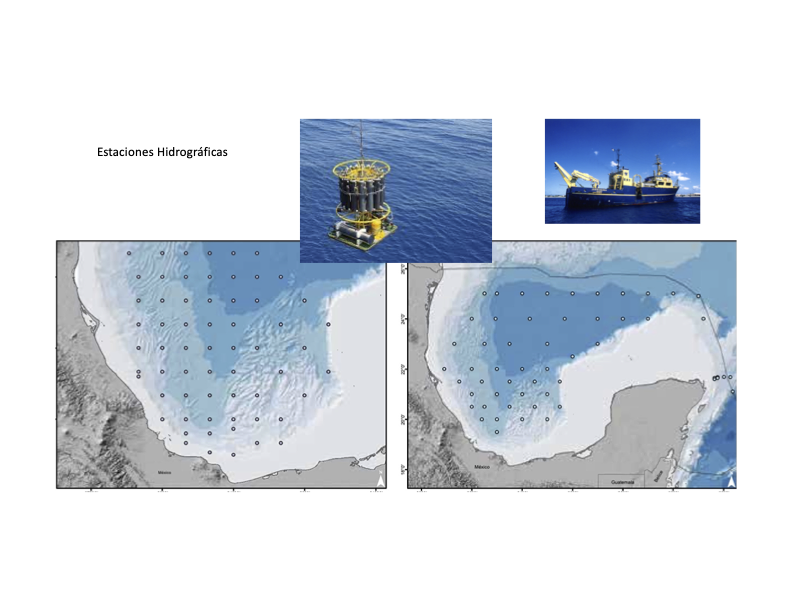
\includepdf[pages={-}]{/Users/julios/curso_analisis_de_datos/Instrumentacion_2023.pdf}

\section{Estadística y conceptos de
probabilidad}\label{estaduxedstica-y-conceptos-de-probabilidad}

\subsection{Porqué estudiar la estadística en oceanografía}

A pesar de nuestra formación determinista a la hora de resolver
problemas matemáticos y aunque consideremos que las ecuaciones de
Navier-Stokes que describen el movimiento del océano son deterministas,
la estadística es ampliamente utilizada en oceanografía debido a
diferentes razones:

\begin{enumerate}
\def\labelenumi{\arabic{enumi}.}
\item
  Para una descripción completa del océano es necesario especificar una
  gran cantidad de variables, muchas de las cuales son desconocidas. Un
  ejemplo de ello son las parametrizaciones que se hacen en oceanografía
  para describir variables que no pueden medirse directamente. Una
  parametrización no es nadammas que un modelo estadístico que explica
  la evolución de una variable dependiente de otras variables
  independientes. Por ejemplo, parametrización del esfuerzo del viento
  en función del corte vertical o parametrización del coeficiente de
  arrastre en función de la velocidad del viento a 10m de la superfície
  del océano.
\item
  El océano es altamente no lineal. La evolución de una cierta variable
  no se puede estudiar de forma aislada.
\end{enumerate}

\vspace{0.5cm}

Ejemplo:\\
Supongamos el término de aceleración horizontal en las ecuaciones de
Navier Stokes para fluidos incompresibles,

\begin{equation}
\frac{\partial{\mathbf {u}_h}}{\partial{t}} + \mathbf {u}_h \cdot {\nabla}_h \mathbf {{u}_h}
\end{equation}

Como ya sabemos por el curso de Mecánica de Fluidos, la aceleración de
un fluido es una derivada material y consta de un término local
(aceleración local) y de un término advectivo o aceleración advectiva.
En general, esta ecuación no se aplica a partículas de agua
individuales.

En oceanografía hablamos de continuo. No estamos interesados en las
características cinemáticas de las partículas individuales sino en la
manifestación promedia del movimiento molecular, es decir, del fluido
como un conjunto o contínuo. Es decir, asumimos que el fluido es
uniforme en el espacio que ocupa sin considerar la estructura molecular.

Por ello debemos de promediar de alguna forma para explicar el
comportamiento conjunto del fluído y no de una partícula de agua
específica? Y como se realiza tal promedio? En general, el promediado se
realiza de tal forma que nos permite separar la larga escala que
trataremos como determinística, de la pequeña escala que consideramos un
proceso aleatorio (turbulento). Supongamos entonces la separación de la
velocidad horizontal en una velocidad promedio y una velocidad
fluctuante alrededor de la media

\[{\mathbf u_h} = <{\mathbf u_h}> + {\mathbf u'_h} \]

donde \$ \textless{} \textgreater{} \$ denotan promedio. Si aplicamos
esta descomposición a la componente \(x\) de la aceleración obtenemos:

\begin{equation}
\frac{\partial <\mathbf {u}>}{\partial t} +  <{\mathbf u}> \cdot  {\nabla} <{\mathbf u} >  + < {\mathbf u'} \cdot {\nabla} \mathbf {u}'> 
\end{equation}

\begin{equation}
 \frac{\partial \mathbf {< u >}}{\partial t} + \nabla \cdot (<{\mathbf u}> \textbf {< u >}) + \nabla \cdot< \mathbf {u'} \mathbf {u}' >
\end{equation}

Donde usamos la ecuación de continuidad

\[ \nabla \cdot (< \mathbf {u} > + \mathbf {u}') =0 \]

para pasar de la primera a la segunda expresión.\\

Inevitablemente, las pequeñas escalas o fluctuaciones respecto a la
larga escala aparecen en la expresión de la aceleración de larga escala.
De forma que la separación que deseamos no es tan simple ya que debemos
de conocer la estadística de la pequeña escala para poder describir la
circulación media.

El término \(<\textbf {u}'_h u'>\) se denomina esfuerzo de Reynolds y
nos informa de la correlación entre las componentes fluctuantes (alta
frecuencia) de la velocidad. Por ejemplo, \(<u'v'> = 0\) significa que
no existe i correlación y hablamos de isotropía. Si \(<u'v'> < 0\),
significa que las fluctuaciones están inversamente correlacionadas,
i.e., anisotropía.

Este es un gran problema no resuelto en la oceanografía física. El
esfuerzo de Reynolds aparece porque la advección es no-lineal de tal
forma que no podemos estudiar la larga escala sin conocer información de
la pequeña escala que es un proceso aleatorio. Por similitud con el
flujo laminar, los términos de esfuerzo de Reynolds se parametrizan
estadísticamente como proporcionales a los gradientes de velocidad. El
factor de proporcionalidad es el coeficiente de viscosidad, en este
caso, turbulento. Es aqui donde utilizar herramientas estadísticas tiene
sentido.

\begin{enumerate}
\def\labelenumi{\arabic{enumi}.}
\setcounter{enumi}{2}
\tightlist
\item
  No podemos controlar las variables oceanográficas; estan en constante
  cambio a medida que el sistema observado evoluciona.
\end{enumerate}

\vspace{0.5cm}

Ejemplo:\\
En el océano coexisten mareas, ondas internas, remolinos, turbulencia de
pequeña escala,\ldots las cuales enmascaran el fenómeno oceanográfico
que estamos interesados en estudiar. Estos procesos incontrolables por
el oceanógrafo en ocasiones es útil considerarlos aleatorios y utilizar
herramientas estadísticas para caracterizarlos.

Imaginemos que queremos conocer cual es la temperatura superficial
promedio en la bahía de Todos Santos. Una forma de proceder sería
promediar todos los datos de temperatura superficial que disponemos de
los últimos 100 años y promediarlos? Pero, ¿es realmente lo que
deseamos? ¿Deberíamos de considerar la estaciones del año y obtener un
pormedio para cada estación? ¿Qué sucede en años Niño, el cual sabemos
que afecta la temperatura del océano? En definitiva, debemos de definir
sobre que conjunto de datos vamos a promediar, y dichos promedio va a
reflejar efectivamente esa elección.\\

Este ejemplo precisa de la distinción entre lo que consideramos nuestra
\emph{señal} (temperatura media) de los procesos que son \emph{ruido}
(Estaciones del año, los años Niño, ondas internas, etc.). De esta
forma, al definir el promedio estamos haciendo explícita la separación
entre \emph{señal} y \emph{ruido}. Finalmente, una vez definido sobre
que promediar, existen en literatura una gran cantidad de herramientas
estadísticas que podemos utilizar. Definir \emph{señal} y \emph{ruido},
y determinar sobre que conjunto de datos vamos a calcular el promedio,
es una tarea difícil. Conocer como debemos muestrear el océano también
debe hacerse cuidadosamente.\\

En oceanografía física se muestrea el océano de forma discontínua, es
decir, se obtienen medidas puntuales en el espacio y en el tiempo. Como
dijimos anteriormente, el océano contiene procesos de diferentes escalas
espaciales y temporales, nolineales, y aleatorios. Es por ello que es
sumamente importante saber escoger el intervalo de muestreo
\(\Delta{t}\) dependiendo del fenómeno que se quiere muestrear. Debemos
de tener en mente que la frecuencia mas alta que podemos resolver es la
frecuencia de Nyquist:

\[f_N=1/(2\Delta{t})\,.\]

Por ejemplo, si medimos a intervalos de \(\Delta{t}=5\,{ h}\) podremos
como máximo resolver procesos que ocurren con frecuencia
\(f_N\le1/10\,{ cph}\). La frecuencia mas baja que podemos resolver va a
depender de la longitud del registro. A esa frecuencia le llamamos
frecuencia fundamental

\[f_0=1/(\Delta{t}N)\,,\]

\{\noindent\}donde \(T=\Delta{t} N\) es la duración del muestreo y N es
el número de muestras o datos. En general, debemos de medir suficiente
tiempo para registrar varios ciclos del fenómeno de estudio para tener
significancia estadística. Por lo tanto, nuestra resolución frecuencial
va a depender del intervalo y duración del muestreo. El cociente
\(f_N/f_0=(1/2\Delta{t})/(1/N\Delta{t})=N/2\) indica el número máximo de
componentes de Fourier que podemos estimar. Una señal periódica se puede
descomponer en la suma de un conjunto (infinito) de funciones
oscilatorias de senos y cosenos o componentes de Fourier. Esto lo
veremos en el capítulo\textasciitilde7. A cada muestreo de un fenómeno
le denominamos realización, y a un conjunto de realizaciones se les
denomina ensamble.

\subsection{Estadística básica}\label{estaduxedstica-buxe1sica}

La estadística trata de describir las características de una población
continua a partir de muestras discretas de la misma. Hablamos de
población y de muestra de una población. Si calculamos, por ejemplo, la
media de una población, estamos calculando un \{parámetro\}. Cuando
calculamos la media de una muestra le llamamos un estadístico de la
población.\\

La estadística nos ayuda a organizar, analizar, presentar datos, y nos
da información de cómo planear la recolección de los mismos, i.e.~a
muestrear.

\begin{center}
%\includegraphics[width=0.5\textwidth]{estadistica_poblacion.pdf}
\end{center}

\vspace{0.5cm}

\begin{enumerate}
\def\labelenumi{\arabic{enumi}.}
\tightlist
\item
  La media:\\
\end{enumerate}

La media de una muestra de N valores \(x_i=x_1,x_2,...,x_N\) es

\begin{equation}
\bar{x}=\frac{1}{N}\sum^N_{i=1}x_i=<x>\,.
\end{equation}

La media debe de diferenciarse de la mediana. La media es el momento de
orden cero. La mediana de una población es aquel valor numérico que
separa el 50\% de valores mas altos del 50\% de valores mas bajos. Se
puede calcular ordenando de menor a mayor el conjunto de valores y
escoger el valor central si el conjunto de datos es impar o el promedio
de los dos centrales si es par.\\

\begin{enumerate}
\def\labelenumi{\arabic{enumi}.}
\setcounter{enumi}{1}
\tightlist
\item
  La varianza:\\
\end{enumerate}

La varianza de un una muestra de N valores \(x_i\) es

\begin{equation}
s^2=\frac{1}{N-1}\sum^N_{i=1}(x_i-\bar{x})^2=<x'^2>\,,
\end{equation}

donde las primas indican fluctuaciones alrededor de la media. La
varianza es una medida de cuán lejos estan los diferentes puntos de la
muestra de la media de la población. La varianza es el segundo momento
alrededor de la media. Al dividir por \(N\) estamos subestimando la
verdaderavarianza de la población. Al dividir por \(N-1\) obtenemos un
estimador insesgado.\\

NOTA: el sesgo de un estimador se refiere a la diferencia entre su
esperanza matemática y el valor numérico (real) del parámetro que se
estima. Un estimador que no tiene sesgo se dice insesgado. Por ejemplo,
para la media:

\[E[x]-\mu \rightarrow {0}\]

\[\bar{x}-\mu \rightarrow {0}\]

EJERCICIO: Demostrar porqué hay que dividir por \(N-1\) en lugar de
\(N\) para que la definición de varianza sea un estimador insesgado.\\

\begin{enumerate}
\def\labelenumi{\arabic{enumi}.}
\setcounter{enumi}{2}
\tightlist
\item
  La desviación típica:\\
\end{enumerate}

Es la raíz cuadrada de la varianza. Se suele escribir como \(\sigma\)
para referirse a la población o como \(s\) en estadística

\begin{equation}
s=\sqrt{s^2}\,.
\end{equation}

\vspace{0.5cm}

\begin{enumerate}
\def\labelenumi{\arabic{enumi}.}
\setcounter{enumi}{3}
\tightlist
\item
  Momentos de orden superior:\\
\end{enumerate}

Podemos definir un momento alrededor de la media como:

\begin{equation}
m_p=\frac{1}{N}\sum^N_{i=1}(x_i-\bar{x})^p=<x'^p>\,.
\end{equation}

De esta forma \(m_2\) es la varianza, \(m_3\) es la asimetría, y \(m_4\)
la curtosis. El momento \(m_3\) indica la asimetría de la muestra
alrededor de la media (\(m_3>0\) implica distribución con cola larga en
la parte positiva y viceversa). \(m_4\) indica el grado de esparcimiento
de las muestras alrededor de la media. Una mayor curtosis indica mayor
concentración de puntos alrededor de la media. Los momentos de orden
superior (\(>2\)) se suelen adimensionalizar dividiendo por la
desviación estándar:

\begin{equation}
    m_3=\frac{1}{N}\sum^N_{i=1}\left[\frac{x_i-\bar{x}}{\sigma}\right]^3=<(x/\sigma)'^3>
\end{equation}

\begin{equation} 
    m_4=\frac{1}{N}\sum^N_{i=1}\left[\frac{x_i-\bar{x}}{\sigma}\right]^4-3=<(x/\sigma)'^4>-3
\end{equation}

donde el factor \(-3\) hace que la curtosis tome el valor cero para una
distribución Normal.

\vspace{0.5cm}

\begin{center}
%\centering
%\includegraphics[width=9cm,angle=0]{skewness.png}
\end{center}

\begin{center}
Figura 1.1. Distribuciones con $m_3<0$ (izquierda) y $m_3>0$ (derecha).
\end{center}

\begin{center}
%\centering
%\includegraphics[width=9cm,angle=0]{Kurtosis.jpg}
\end{center}

\begin{center}
Figura 1.2. Distribuciones con diferentes grados de curtosis; $m_4>0$ (Leptocúrtica),
$m_4=0$ (Normal o Mesocúrtica), y $m_4<0$ (Platicúrtica).
\end{center}

\vspace{0.5cm}

\begin{enumerate}
\def\labelenumi{(\arabic{enumi})}
\setcounter{enumi}{4}
\tightlist
\item
  Covarianza y correlación:\\
\end{enumerate}

La covarianza entre dos variables \(x\) e \(y\) puede definirse como un
estadístico que relaciona \(x\) e \(y\) de la siguiente forma

\[C_{xy}=<x'y'>=<(x-\bar{x})(y-\bar{y})>=\frac{1}{N-1}\sum\limits^N_{i=1} (x_i-\bar{x})(y_i-\bar{y})\,.\]

La correlación es la covarianza normalizada

\[\rho_{x y}=\frac{C_{x y}}{s_x s_y}=\frac{<x' y'>}{\sqrt{<x'^2><y'^2>}}\,. \]

Consideremos el modelo estadístico lineal de media cero (es una recta
que pasa por \((\overline{x},\overline{y})=(0,0)\))

\[\hat{y}=\alpha x\,,\]

donde \(\alpha\) es una constante. El error cometido por este estimador
se define como el error cuadratico medio

\[\epsilon=<(\hat{y}-y)^2>=\alpha^2<x^2>+<y^2>-2\alpha<xy>\]

y si queremos minimizar dicho error entonces tenemos que encontrar que
\(\alpha\) es el que provoca que la derivada
\(\partial{\epsilon}/\partial{\alpha}\rightarrow{0}\). Es decir

\[\partial{\epsilon}/\partial{\alpha}=2\alpha<x^2>-2<xy>=0\,,\]

y el \(\alpha\) es

\[\alpha=\frac{<xy>}{<x^2>}\,.\]

El error cuadrático mínimo se encuentra substituyendo el valor de
\(\alpha\) en la expresión del error \(\epsilon\) de arriba

\[\epsilon=\frac{<xy>^2}{<x^2>} + <y^2> - 2\frac{<xy>^2}{<x^2>}=
           <y^2>\left(\frac{<xy>^2}{<x^2><y^2>}+1-2\frac{<xy>^2}{<x^2><y^2>}\right)=\]

\[=<y^2>(1-\rho^2_{xy})\,.\]

Si \(\rho^2_{xy}=1\) entonces el error es cero, es decir, mínimo error.
Opuestamente, si \(\rho^2_{xy}=0\) entonces el error es igual a la
varianza, es decir, máximo error. Si \(\rho\) toma valores intermedios,
i.e., \(\rho^2_{xy}=0.5\), entonces el error es \(\epsilon=0.5<y^2>\),
es decir, el error del modelo lineal es un \(50\%\) de la varianza. Por
lo tanto, la correlación al cuadrado puede definirse también ciomo la
eficiencia relativa del estimador \(\hat{y}^2\) o la fracción de
varianza explicada por el modelo lineal

\[\rho^2_{xy}=\frac{<\hat{y}^2>}{<y^2>}=\frac{{varianza\,\,\,explicada}}{{ varianza\,\,\,total}}\,.\]

A este parámetro se le puede encontrar en literatura inglesa como
\emph{skill} del modelo lineal.

\section{Probabilidad}\label{probabilidad}

\vspace{0.5cm}

\subsection{Distribuciones de
probabilidad:}\label{distribuciones-de-probabilidad}

La \{función de distribución acumulativa\} \(D_x(r)\) se define como la
probabilidad que una variable aleatoria \(x\) sea menor o igual a \(r\),
es decir, \(P(x\le r)\). Matemáticamente:

\[D(x)=\int^r_{-\infty}F(x)dx\,,\]

donde

\[F(x)=\frac{d}{dx} D(x)\]

es la función de densidad de probabilidad (PDF, por su siglas en
inglés). La PDF nos informa de la probabilidad que \(x\) sea igual a un
cierto valor \(r\), \(P(x=r)\).\\

\{\noindent\} Algunas propiedades de \(D(x)\):

\hfill\break
* \(D(r)\le D(s)\,\,\,{ if}\,\,\,r\le s\)\\
* \(D(-\infty)=0\)\\
* \(D(\infty)=1\)\\

Algunas propiedades de \(F(x)\):\\

\begin{enumerate}
\def\labelenumi{(\arabic{enumi})}
\tightlist
\item
  \(F(x)\ge0\)\\
\item
  \(\int^{\infty}_{-\infty} F(x) dx=1\)\\
\end{enumerate}

La probabilidad que una variable aleatoria \(x\) este contenida en el
intervalo \([r,r+dr]\) es la integral de la función de densidad de
probabilidad \[P(r\le x\le r+dr)=\int^{r+dr}_r F(x)dx\,.\]

Ambas definiciones son parecidas aunque no son lo mismo. Para ello
veamos el ejemplo de la suma del lanzamiento de dos dados al aire.\\

\begin{center}
%\centering
%\includegraphics[width=10cm,angle=0]{prob_acumul_dados.png}
\end{center}

La densidad de probabilidad de que la suma de los dos dados sea 7 es
máxima y que sea 2 o 12 es mínima. Este ejemplo describe dos propiedades
fundamentales de funciones de probabilidad discretas: (i)
\(P(X=x) \ge 0\) y (ii)\(\sum{P(x)}=1\). La distribución de probabilidad
acumulativa y la función de densidad de probabilidad tienen las
siguientes distribuciones\\

\begin{center}
%\centering
%\includegraphics[width=10cm,angle=0]{prob_acumul_dados_figure.png}
\end{center}

\vspace{0.5cm}

\{\noindent\} Momentos estadísticos de una función de densidad de
probabilidad:\\

Los momentos centrados (o alrededor de la media) de una distribución de
probabilidad se definen como

\[m_r=E[(x-E[x])^r]=\int^{\infty}_{-\infty} (x-\mu)^rF(x)dx\,.\]

Como caso particular, los momentos alrededor del origen (i.e.,
\(\mu=0\)) son: \[m^0_r=E[x^r]=\int^{\infty}_{-\infty} x^rF(x)dx\,.\]

Entonces, los primeros tres momentos centrados se definen como

\[m_0=E[(x-E[x])^0]=E[1]=\int^{\infty}_{-\infty}F(x)dx=1\,,\]
\[m_1=E[(x-E[x])^1]=E[x]-\mu=\int^{\infty}_{-\infty} (x-\mu)^1 F(x)dx=0\,,\]
\[m_2=E[(x-E[x])^2]=E[x^2 + E[x]^2 -2xE[x]]=
      E[x^2]+E[x]^2-2E[x]E[x]=\]
\[E[x^2]-E[x]^2=\underbrace{E[x^2]}_{\sigma^2}-\mu^2=\int^{\infty}_{-\infty} (x-\mu)^2 F(x)dx=\sigma^2-\mu^2\,.\]

Los momentos alrededor de cero (\(\mu=0\)) tambien pueden ser
estandarizados:
\[m^*_r=m_r/\sigma^r=\frac{E[(x-E[x])^r]}{(\underbrace{E[(x-E[x])^2]}_{\sigma^2})^{r/2}}\,.\]

Los cuatro primeros momentos estadísticos alrededor de cero
estandarizados son:
\[m^*_1=m_1/\sigma^1=\frac{E[(x-\mu)^1]}{(E[(x-\mu)^2])^{1/2}}=\frac{\mu-\mu}{\sqrt{E[(x-\mu)^2]}}=0\,,\]
\[m^*_2=m_2/\sigma^2=\frac{E[(x-\mu)^2]}{(E[(x-\mu)^2])^{2/2}}=1\,,\]
\[m^*_3=m_3/\sigma^3=\frac{E[(x-\mu)^3]}{(E[(x-\mu)^2])^{3/2}}\,,\]
\[m^*_4=m_4/\sigma^4=\frac{E[(x-\mu)^4]}{(E[(x-\mu)^2])^{4/2}}\,.\]

\vspace{0.5cm}

\begin{enumerate}
\def\labelenumi{\arabic{enumi}.}
\tightlist
\item
  Distribución uniforme:\\
  La distribución de probabilidad uniforme viene dada por
  \[F(x)=\frac{1}{b-a}\,\,\,, a \le x \le b\]
  \[=0,\,\,\,\,fuera\,\,del\,\,intervalo\]
\end{enumerate}

Se deduce de la expresión de área de un cuadrado:

\[Area=base*altura=(b-a)F(x)=1\]

La función de distribución acumulativa es \[D(x)=0,\,\,\,x<a\]
\[D(x)=\frac{x-a}{b-a},\,\,\,a \le x \le b\] \[D(x)=1,\,\,\,x \ge b\]\\

\begin{center}
%\centering
%\includegraphics[width=10cm,angle=0]{distribucion_uniforme.png}
\end{center}

La media es \(\mu=(b+a)/2\) y la varianza es
\(\sigma^2=1/3(a^2 + b^2 +ab)\). Demostración:\\

\{\noindent\} Los momentos estadísticos alrededor del origen de la
distribución uniforme son
\[m^0_r=E[x^r]=\int^{\infty}_{-\infty} x^rF(x)dx=\int^{b}_{a} \frac{x^r}{b-a}dx=\]

\[\frac{1}{b-a}\int^{b}_{a}x^r dx=\frac{1}{b-a}\left[\frac{x^{r+1}}{r+1}\right]^b_a=
      \frac{1}{b-a}\left[\frac{b^{r+1}}{r+1}-\frac{a^{r+1}}{r+1}\right]=\frac{b^{r+1}-a^{r+1}}{(b-a)(r+1)}\]

y por lo tanto la media es

\[m^0_1=E(x)=\frac{b^2-a^2}{2(b-a)}=\frac{(b-a)(b+a)}{2(b-a)}=\frac{b+a}{2}\,,\]

y la varianza

\[m^0_2=E(x^2)=\frac{b^3-a^3}{3(b-a)}=\frac{(b-a)(a^2+b^2+ab)}{3(b-a)}=\frac{1}{3}(a^2 + b^2 +ab)\,.\]

Ejemplo de distribución uniforme: La ruleta rusa. Supongamos que puede
tomar 360 valores, es decir, \(0 \le x \le 360\). Entonces

\[F(x)=\frac{1}{360},\,\,\,0 \le x \le 360\,,\]

y, por ejemplo, la probabilidad de que la bola caiga entre el 50 y el
360 es

\[P(50\le x \le 360)=\int^{360}_{50}\frac{1}{360}dx=\frac{1}{360}\left[x\right]^{360}_{50}=\frac{310}{360}=0.8611\,(\sim86\%).\]

La función de distribución acumulativa es

\[D(x)=0,\,\,\,x<0\] \[D(x)=\frac{x}{360},\,\,\,0 \le x \le 360\]
\[D(x)=1,\,\,\,x \ge 360\]

\vspace{0.5cm}

\begin{enumerate}
\def\labelenumi{\arabic{enumi}.}
\setcounter{enumi}{1}
\tightlist
\item
  Distribución normal o Gaussiana:\\
\end{enumerate}

La distribución normal es una de las distribuciones mas recurrente en la
naturaleza. En general cualquier variable aleatoria medida,
especialmente aquellas que son suma de otras variables aleatorias, tiene
una distribución normal alrededor de la media

\[F(x)=\frac{1}{\sigma\sqrt{2\pi}}{exp}
   \left\{ -\frac{(x-\bar{x})^2}{2\sigma^2} \right\}\,.\]

\begin{center}
%\centering
%\includegraphics[width=6cm,angle=0]{normal_distribution_PDF}
\end{center}

La distribución de función acumulativa normal se obtiene integrando la
expresión de arriba. Para ello vamos a realizar el cambio de variable
(que no es nada mas que estandarizar la variable aleatoria x)

\[z=\frac{x-\bar{x}}{\sigma\sqrt{2}}\] y
\[dz=\frac{dx}{\sigma\sqrt{2}}\,,\]

de lo que se deduce

\[D(z)=\frac{\sigma\sqrt{2}}{\sigma\sqrt{2\pi}}\int^z_{-\infty} {exp}
  \left\{ -z^2 \right\}dz =
  \frac{1}{\sqrt{\pi}}\int^z_{-\infty} {exp}
  \left\{ -z^2 \right\} dz\,,\]

donde
\(\frac{2}{\sqrt{\pi}}\int^z_{0}{exp}\left\{ -t^2 \right\}dt={erf}(z)\,.\)

\begin{center}
%\centering
%\includegraphics[width=7cm,angle=0]{normal_cumulative}
\end{center}

Los momentos estadísticos alrededor del origen de la función de
distribución Normal son

\[m^0_r=E[x^r]=\int^{\infty}_{-\infty} x^rF(x)dx=\frac{1}{\sigma\sqrt{2\pi}}\int^{\infty}_{-\infty}x^r{exp}
   \left\{ -\frac{(x-\bar{x})^2}{2\sigma^2} \right\} dx\]

Hagamos el cambio de variable

\[u=\frac{x-\bar{x}}{\sigma\sqrt{2}}\] \[du=\frac{dx}{\sigma\sqrt{2}}\]

Si substituimos en la expresión de \(m_r\) obtenemos

\[m^0_r=\frac{\sigma\sqrt{2}}{\sigma\sqrt{2\pi}}\int^{\infty}_{-\infty}
  \left( \sigma \sqrt{2}u+\bar{x}\right)^r{e}^{-u^2}du=
  \frac{1}{\sqrt{\pi}}\int^{\infty}_{-\infty}\left( \sigma \sqrt{2}u+\bar{x}\right)^r{e}
   ^{-u^2}du\,.\]

\vspace{0.25cm}

\textbf{Ejercicio}: Deducir los momentos estadísticos de orden 1 y 2 de
la distribución Normal, es decir, la media y la varianza. Integrales
útiles:

\[\int e^{-ax^2}dx=\frac{\sqrt{\pi}}{2\sqrt{a}}{erf}(x\sqrt{a})\]
\[\int xe^{-ax^2}dx=-\frac{1}{2a}e^{-ax^2}\,,\]

donde la función de error se define cómo:

\[erf(z)=\frac{2}{\sqrt{\pi}}\int_0^z e^{-t^2} dt\,.\]

La función de error cumple las siguientes identidades:
\[{erf}(0)=\frac{2}{\sqrt{\pi}}\int_0^0 e^{-t^2} dt=0\],
\[{erf}(\infty)=\frac{2}{\sqrt{\pi}}\underbrace{\int_0^\infty e^{-t^2} dt}_{\frac{\sqrt{\pi}}{2}}=1\].
\[{erf}(-\infty)=\frac{2}{\sqrt{\pi}}\underbrace{\int_0^{-\infty} e^{-t^2} dt}_{-\frac{\sqrt{\pi}}{2}}=-1\].

\vspace{0.25cm}

\textbf{Respuesta}: La media y la varianza son

\[m^0_1=E(x)=\mu\,\,\,\,\,\,;\,\,\,\,\,\,m_1=0\]
\[m^0_2=Var(x)=\mu^2 + \sigma^2\,\,\,\,\,\,;\,\,\,\,\,\,m_2=\sigma^2\]

\vspace{0.25cm}

Deducción de la media: El momento de orden 1 centrado es:

\[m_1=\frac{\sigma\sqrt{2}}{\sqrt{\pi}}\int^{\infty}_{-\infty}u{e}
   ^{-u^2}du=-\frac{\sigma\sqrt{2}}{2\sqrt{\pi}}{e}
   ^{-u^2}\Big|^{\infty}_{-\infty}=0\,.\]\\
y alrededor de cero (momentos crudos):

\[m^0_1=\frac{1}{\sqrt{\pi}}\int^{\infty}_{-\infty}(\sigma \sqrt{2} u + \mu){e}
   ^{-u^2}du=\frac{\sigma\sqrt{2}}{\sqrt{\pi}}\int^{\infty}_{-\infty}u{e}
   ^{-u^2}du + \frac{1}{\sqrt{\pi}}\int^{\infty}_{-\infty}\mu{ e}
   ^{-u^2}du=\]\\
\[=\underbrace{\frac{\sigma\sqrt{2}}{\sqrt{\pi}}\left( -\frac{1}{2}{ e}
   ^{-u^2}\right)}_{0} \Big|^{\infty}_{-\infty}+
   \frac{\mu}{\sqrt{\pi}}\left( \frac{\sqrt{\pi}}{2}{ erf}(u)\right) \Big|^{\infty}_{-\infty}=
   \frac{\mu}{2}[1-(-1)]=\mu\,,\]

\vspace{0.25cm}

\textbf{Deducción de la varianza}:

El momento de orden 2 centrado es:\\

\[m_2=\frac{(\sigma\sqrt{2})^2}{\sqrt{\pi}}\int^{\infty}_{-\infty}u^2{ e}^{-u^2}du\]

\[x=u \rightarrow dx=du\]
\[dy=u{ e}^{-u^2} \rightarrow y=\frac{1}{2}{ e}^{-u^2}\]

\[m_2=\frac{2\sigma^2}{\sqrt{\pi}}\left[ -\frac{1}{2}{ e}^{-u^2}
      \Big|^{\infty}_{-\infty} +\frac{\sqrt{\pi}}{4} { erf}(u)\Big|^{\infty}_{-\infty}\right]=
  \frac{2\sigma^2}{\sqrt{\pi}}\left[0 + \frac{\pi}{4}\left({ erf}(\infty) - { erf}(-\infty) \right)
  \right]=\]
\[=\frac{2\sigma^2}{\sqrt{\pi}}\left[ \frac{\pi}{4}+\frac{\pi}{4}\right]=\sigma^2\]\\

y alrededor de cero (momentos crudos):

\[m^0_2=\frac{1}{\sqrt{\pi}}\int^{\infty}_{-\infty}(\sigma \sqrt{2} u + \mu)^2{ e}^{-u^2}du=
   \frac{1}{\sqrt{\pi}}\int^{\infty}_{-\infty}2\sigma^2 u^2{ e}^{-u^2}du +\]
\[ +\frac{\mu^2}{\sqrt{\pi}}\int^{\infty}_{-\infty}{ e}^{-u^2}du
   +\frac{2\sigma\sqrt{2}\mu}{\sqrt{\pi}}\int^{\infty}_{-\infty}u{ e}^{-u^2}du=\]

\[
   =\underbrace{\frac{2\sigma^2}{\sqrt{\pi}}\int^{\infty}_{-\infty}u^2{ e}^{-u^2}du}_{m_2=\sigma^2}
   +\mu \underbrace{\frac{1}{\sqrt{\pi}}\int^{\infty}_{-\infty}\mu{ e}^{-u^2}du}_{m_1^0=\mu}+
   +2\mu \underbrace{\frac{\sigma\sqrt{2}}{\sqrt{\pi}}\int^{\infty}_{-\infty}u{ e}^{-u^2}du}_{m_1=0}= \sigma^2+\mu^2\,,\]\\

La probabilidad de que una variable normalmentedistribuida caiga en una
desviación estándar de su valor medio viene dada por
\[P(-1\le z \le 1)=\int^{+1}_{-1} F(z) dz=\frac{1}{\sqrt{2\pi}}\int^{+1}_{-1}e^{-\frac{1}{2}z^2}dz=\]
\[=\frac{1}{\sqrt{2\pi}}\frac{\sqrt{\pi}}{2\sqrt{1/2}}\left[{ erf}({z\sqrt{1/2}})\right]^1_{-1}=
   \frac{1}{2}\left[{ erf}({1/\sqrt{2}})-{ erf}({-1/\sqrt{2}}) \right]=\]
\[=\frac{1}{2}\left[0.6827-(-0.6827)\right]=0.6827\,(~68.27\%)\,,\]\\

y similarmente para 2 y 3 desviaciones estándar\\

\[P(-2\le z \le 2)=\int^{+2}_{-2} F_x(z) dz=95.45\%\]
\[P(-3\le z \le 3)=\int^{+3}_{-3} F_x(z) dz=99.73\%\,.\]

Entonces solo hay un \(4.55\%\) de probabilidad de que una variable
normalmente distribuida caiga fuera de dos desviaciones estándar
respecto de la media. Puesto que es una probabilidad con 2 colas, la
probabilidad de que una variable normal exceda su media por mas de
\(2\sigma\) es la mitad de esto, es decir \(2.275\%\), ya que la
distribución normal es simétrica.\\
En la práctica una PDF se calcula como un histograma escalado. Es por
ello que necesitamos escoger el tamaño y localización de los bins en el
histograma. La demo muestra las consecuencias de esta elección
(pdf\_demo.m).

\begin{center}
%\centering
%\includegraphics[width=12cm,angle=0]{probability_normal}
\end{center}

\vspace{0.5cm}

\begin{enumerate}
\def\labelenumi{\arabic{enumi}.}
\setcounter{enumi}{2}
\tightlist
\item
  Distribución de Poisson:\\
\end{enumerate}

La distribución de Poisson expresa la probabilidad de que ocurra un
determinado número de eventos durante un cierto intervalo en el tiempo o
distancia en el espacio. Se usa generalmente para la ocurrencia de
sucesos con muy poca probabilidad o muy ``raros'\,'. La expresión para
la función acumulativa es:

\[D(x)=P(x \le r)=e^{-\lambda}\sum^{|r|}_{k=0}\frac{\lambda^k}{k!}\,,\]

donde \(\lambda\) es el valor promedio

\begin{center}
%\centering
%\includegraphics[width=6cm,angle=0]{distribucion_Poisson_CDF}
\end{center}

y la función de densidad de probabilidad

\[F(x)=P(x=k)=\frac{{\lambda}^k e^{-\lambda}}{k!}\]

\begin{center}
%\centering
%\includegraphics[width=6cm,angle=0]{distribucion_Poisson_PDF}
\end{center}

Los momentos estadísticos alrededor del origen de la función de
distribución de Poisson se pueden calcular directamente con sumatorios y
expansion de Taylor:

\[m^0_r=E[x^r]=\sum k^r P(X=k)=\sum_{k\ge0} k^rF(x)= \sum_{k\ge0} k^r\frac{{\lambda}^k e^{-\lambda}}{k!}=\]
\[=\lambda e^{-\lambda}\sum_{k \ge 0}\frac{k^r}{k!}\lambda^{k-1}\]

\{\noindent\}Veamos el momento de orden 1 alrededor del orígen:

\[m^0_1=E[x]=\lambda e^{-\lambda}\sum_{k \ge 0}\frac{k}{k!}\lambda^{k-1}=
 \lambda e^{-\lambda}\sum_{k \ge 1}\frac{k}{(k-1)!k}\lambda^{k-1}=
 \lambda e^{-\lambda}\sum_{k \ge 1}\frac{1}{(k-1)!}\lambda^{k-1}\]
\[=\lambda e^{-\lambda}\sum_{j \ge 0}\frac{\lambda^{j}}{j!}\,,\] para
\(j=k-1\). Finalmente expandiendo en series de Taylor la función
exponencial

\[e^{\lambda}=\sum_{j \ge 0}\frac{1}{j!}\lambda^{j}\], obtenemos:

\[m^0_1=\lambda e^{-\lambda}e^{\lambda}=\lambda\]

Ejercicio: Demostrar que el momento estadístico alrededor del origen de
orden 2 de la distribución de Poisson es igual a
\(m^0_2=\lambda+\lambda^2\).

\[m^0_2=E[x^2]=\lambda e^{-\lambda}\sum_{k \ge 0}\frac{k^2}{k!}\lambda^{k-1}=
               \lambda e^{-\lambda}\left[ \sum_{k \ge 1}(k-1)\frac{1}{(k-1)!}\lambda^{k-1} +
                                      \sum_{k \ge 1} \frac{1} {(k-1)!} \lambda^{k-1} \right]=\]

\[= \lambda e^{-\lambda}\left[ \lambda \sum_{k \ge 2}\frac{1}{(k-2)!}\lambda^{k-2} + \sum_{k \ge 1}\frac{1}{(k-1)!}\lambda^{k-1}\right]=\]
\[= \lambda e^{-\lambda}\left[ \lambda \sum_{j \ge 0}\frac{1}{j!}\lambda^{j} + \sum_{i \ge 0}\frac{1}{(i)!}\lambda^{i}\right]=
\lambda e^{-\lambda} \left[\lambda e^{\lambda} + e^{\lambda}\right]=\]

\[=\lambda (\lambda +1)=\lambda^2 + \lambda\,.\]

En el casso que fuera el momento de orden 2 centrado se escribiría:

\[E[(x-E[x])^2]=E[x^2]-(E[x])^2=\lambda^2 + \lambda - (\lambda)^2=\lambda\,.\]

\vspace{0.25cm}

\textbf{Ejemplo}: En los últimos 160 años, han sucedido 680 tormentas
intensas en el Golfo de México, incluyendo depresiones, tormentas
tropicales, y huracanes. Asumimos que la frecuencia de ocurrencia de una
tormenta intensa en el Golfo de México sigue una distribución de Poisson
(eventos ``raros'', poco frecuentes). Calcula la probabilidad de que
ocurran 2 huracanes en 1 año:\\

\begin{enumerate}
\def\labelenumi{(\alph{enumi})}
\item
  El número promedio de tormentas intensas por año es:
  \(\mu=680/160=4.25\) huracanes/año.
\item
  La probabilidad de que ocurran 2 huracanes en 1 año es:
\end{enumerate}

\[P(x=2)=\frac{{\lambda}^2 e^{-\lambda}}{2!}=\frac{{4.25}^2 e^{-4.25}}{2!}=0.1288\,(\sim12\%)\]

La probabilidad es muy baja debido a que exigimos que sean exactamente 2
huracanes en un año y no, por ejemplo, \(>2\). En el segundo caso, la
probabilidad aumentaría considerablemente

\[P(x>2)=P(x=3)+P(x=4)+....=1-P(x\le 2)=1-[P(x=0)+P(x=1)+P(x=2)]=\]
\[=1-[0.0143+0.0606+0.1288]=1-0.2037=0.7963\,(\sim80\%)\]

\vspace{0.5cm}

\begin{enumerate}
\def\labelenumi{\arabic{enumi}.}
\setcounter{enumi}{3}
\tightlist
\item
  Distribución Binomial:
\end{enumerate}

Supongamos que tenemos un conjunto de \(n\) tiradas en los cuales pueden
suceder únicamente dos cosas:
\texttt{acierto\textquotesingle{}\ o}fallo'. La probabilidad de acertar
en una tirada es p=P. Si \(X\) es el número total de aciertos en \(n\)
tiradas, entonces la probabilidad de que el número de aciertos sea \(k\)
es:

\[P(X=k)=\left( \begin{array}{c}
 n \\ k
       \end{array} \right)
p^k (1-p)^{n-k}, \, k=0,1,2,3,....,n\,,\]

\noindent\}donde la expresión

\[\left( \begin{array}{c}
 n \\ k
       \end{array} \right)=C(n,k)\equiv\frac{n!}{(n-k)!k!}\,,\]\\

es el número de diferentes combinaciones de grupos de k objetos que
pueden ser elegidos de un conjunto total de n objetos. Estos números se
denominan coeficientes binomiales. La probabilidad de que el número de
aciertos caiga en un rango de valores es

\[P(a\le X\le b)=\sum^b_a P(X)\]

\vspace{0.5cm}

Ejemplo 1: ¿Cual es la probabilidad de obtener exactamente 6 caras de 10
lanzamientos de moneda? Respuesta:

\[P(x=6) = C(10,6)0.5^6(1-0.5)^{10-6} = \frac{10!}{(10-6)!6!}0.5^6(1-0.5)^{10-6} \simeq 0.205\]

\vspace{0.5cm}

\{\noindent  Ejemplo 2:\} ¿Cual es la probabilidad de obtener mas de 15
caras de 20 lanzamientos de moneda? Respuesta:

\[\sum^{20}_{k=16} \left( \begin{array}{c} 20 \\ k
       \end{array} \right) 0.5^k(1-0.5)^{20-k}=0.006\,.\]

Si realizas esta operación a mano se vuelve muy tediosa. Es por ello que
se utiliza la aproximación Normal a la distribución Binomial
(DeMoivre-Laplace).

\vspace{0.5cm}

\{\noindent\} \textbf{Teorema de DeMoivere-Laplace} (aproximación de
Binomial a Normal)\\

La distribución binomial de una variable X definida por n tiradas
independientes cada una de las cuales tienen una probabilidad \(p\) de
acertar, es aproximadamente una distribución Normal de media \(np\) y
desviación típica \(\sqrt{np(1-p)}\), cuando n es suficientemente
grande. Entonces se deduce que para cualquier número a y b,

\[lim_{n\rightarrow\infty} P \left( a<\frac{X-np}{\sqrt{np(1-p)}}<b\right)= \frac{1}{\sqrt{2\pi np(1-p)}}\int^b_a exp-\left[\frac{(x-np)^2}{2np(1-p)}\right]dx\,.\]\\

Esto significa que el estadístico, \(\frac{X-np}{\sqrt{np(1-p)}}\) ,
tiene una distribución Normal. Este teorema es un caso particular del
teorema del límite central y nos permite de simplificar la solución de
un problema binomial.

\vspace{0.5cm}

\{\noindent\} \textbf{Ejemplo de la aproximación Normal a la
distribución Binomial}:\\

El 2\% de los XBTs fabricados por una empresa presentan defectos. Si
hemos adquirido 2000 XBTs, ¿Cual es la probabilidad de que haya menos de
50 defectuosos?\\

Respuesta: Se trata de una distribución binomial ya que solo pueden ser
defectuosos o no defectuosos. La probabilidad que sea defectuoso es
\(p=0.02\) (2\%) y \(n=2000\), lo que nos da una distribución Binomial
\(B(2000,0.02)\). Puesto que la \(n\) es grande podemos hacer una
aproximación a la distribución Normal. Calculamos la media y desviación
estándar de la distribución Normal \(\mu=np=200*0.02=40\) y
\(\sigma=\sqrt{np(1-p)}=\sqrt{2000*0.02*(1-0.02)}=6.26\) \(x\) es
\(B(2000,0.02)\) y \(x_N\) es \(N(40,6.26)\).\\
La probabilidad que \(x<50\) es \[p(x<50)=p(x_N\le 49)\,,\] y si
estandarizamos
\[p(x_N\le 49)=p\left(z\le \frac{49-40}{6.26} \right)=p(z\le 1.44)=0.9251\,.\]

\vspace{0.5cm}

\{\noindent\} EJERCICIOS de estadística y probabilidad:\\

\vspace{0.5cm}

Ejercicio 1: Calcule E{[}x{]} si x tiene la función de densidad de
probabilidad

\[ f(x)=\Bigg(\begin{array}{c}
 \frac{1}{4}xe^{-\frac{x}{2}}\,\,\,\,\,,x>0 \\ 0 \,\,\,\,\,,otherwise
\end{array})\,.\]

La esperanza E{[}x{]} de la función \(f(x)\) es entonces

\[E[x]=\int^\infty_0 x\left(\frac{1}{4}xe^{-\frac{x}{2}}\right)dx
      =\frac{1}{4}\int^\infty_0 x^2e^{-\frac{x}{2}}dx\,.\]

Definamos \(y=x/2\); entonces \(x=2y\) y \(dx=2dy\) y obtenemos

\[E[x]=\frac{1}{4}\int^\infty_0 x^2e^{-\frac{x}{2}}dx
        =\frac{1}{4}\int^\infty_0 (2y)^2e^{-y}2dy
    =2\int^\infty_0y^2e^{-y}dy\,.\] Vamos ahora a resolver la integral
por partes. Hacemos la siguiente sustitución: \(u=y^2\), \(dv=e^{-y}\) y
por ende \(du=2ydy\) y \(v=-e^{-y}\). La integral se puede reescribir
usando la expresión general de integración por partes
\(h(x)=uv-\int vdv\):

\[E[x]=2\int^\infty_0y^2e^{-y}dy=2\left[ -y^2e^{-y}-\int-e^{-y}(2y)dy\right]
      =2\left[ -y^2e^{-y}+2\int ye^{-y}dy\right]\,.\]

Integramos de nuevo por partes. Usa \(u=y\), \(dv=e^{-y}\) y entonces
\(du=dy\) y \(v=-e^{-y}\)

\[E[x]=2\left[ -y^2 e^{-y} + 2 \Big\{ -y e^{-y} - \int -e^{-y}dy \Big\} \right]=\]
\[=2\left[ -y^2 e^{-y} + 2 \Big\{ -y e^{-y} - e^{-y}         \Big\} \right]=\]

\[=-2y^2e^{-y}-4ye^{-y}-4e^{-y}=\]
\[=\left[ -2e^{-y}(y^2+2y+2) \right]^{\infty}_0=\]
\[=\lim_{n \to\infty}\left[ -2e^{-y}(y^2+2y+2) \right]-\left[ -2e^{-y}(y^2+2y+2) \right]_{y=0}\,.\]

El límite es ahora del tipo \(\infty/\infty\) y entonces usamos la regla
de l'Hopital
\[E[x]=-2\lim_{y \to\infty}\frac{2y+2}{e^y}+2\left[e^{-y}(y^2+2y+2) \right]_{y=0}\]
Usamos la regla de l'Hopital de nuevo

\[E[x]=-2\lim_{y \to\infty}\frac{2}{e^y}+2\left[e^{-y}(y^2+2y+2) \right]_{y=0}=0+2\left[e^{-y}(y^2+2y+2) \right]_{y=0}=4\]

\vspace{0.5cm}

\{\noindent\} Ejercicio 2: Calcule E{[}x{]} si x tiene la función de
densidad de probabilidad

\[f(x)=\Bigg\{\begin{array}{c}
 c(1-x^2)\,\,\,\,\,,-1<x<1 \\ 0 \,\,\,\,\,,otherwise
       \end{array} \,.\]

\[E[x]=\int^1_{-1} x[c(1-x^2)]dx=c \int^1_{-1} x[(1-x^2)]dx=\]
\[=c \int^1_{-1} x-x^3dx=c\left[\frac{x^2}{2}+\frac{x^4}{4}\right]^{1}_{-1}=0\]

\vspace{0.5cm}

\{\noindent\} Ejercicio 3: Calcule E{[}x{]} si x tiene la función de
densidad de probabilidad

\[f(x)=\Bigg\{\begin{array}{c}
 \frac{5}{x^2}\,\,\,\,\,,x>5 \\ 0 \,\,\,\,\,,x\le5
       \end{array} \,.\]

\[E[x]=\int^{\infty}_{5}x\frac{5}{x^2}dx=\int^{\infty}_{5}\frac{5}{x}dx=5\int^{\infty}_{5}\frac{1}{x}dx\]
\[=5[lnx]^{\infty}_5=5\left[\Big(\lim_{x \to\infty} ln{x}\Big)-ln{5}\right]\rightarrow \infty\]

\vspace{0.5cm}

\noindent  {Ejercicio 4:} La variable aleatoria \(x\) tiene la siguiente
función de densidad de probabilidad

\[f(x)=\Bigg\{\begin{array}{c}
          k(2x+3)\,\,\,\,\,-1\le x \le 2 \\ 0 \,\,\,\,\,otherwise
         \end{array} \,.\]

\begin{itemize}
\item ?`Cuál es el valor de k?

$$\int^{\infty}_{-\infty} k(2x+3)dx=1$$

$$\int^{2}_{-1} k(2x+3)dx=(kx^2 +3kx)\Big|^{2}_{-1}=kx(3+x)\Big|^{2}_{-1}=10k+2k=1$$

$$12k=1 \rightarrow k=\frac{1}{12}$$


\item Calcula $E[x]$

$$E[x]=\int^{2}_{-1}x k(2x+3)dx=2k\frac{x^3}{3}\Bigg|^{2}_{-1} + 3k\frac{x^2}{2}\Bigg|^{2}_{-1}=$$
$$=k\left[ \frac{18}{3} + \frac{9}{2}\right]=\frac{21}{24}\,.$$

\end{itemize}

\vspace{0.5cm}

\noindent  {Ejercicio 5:} Sea la función \(g(x)\) dada por

\[g(x)=\Bigg\{\begin{array}{c}
 x+2\alpha\,\,\,\,\,,x\le-\alpha \\
 x \,\,\,\,\,,-\alpha \le x \le \alpha \\
 x-2 \alpha \,\,\,\,\,,x>\alpha
       \end{array} \,,\]

donde asumimos que x esta normalmente distribuida. Calcula la media de
\(g(x)\).

\[E[g(x)]=\int^{\infty}_{-\infty} g(x) F(x) dx=\int^{-\alpha}_{-\infty} (x+2\alpha) F(x) dx +
\int^{\alpha}_{-\alpha} x F(x) dx + \int^{\infty}_{\alpha} (x-2\alpha) F(x) dx=\]
\[=\int^{-\alpha}_{-\infty} x F(x) dx + \int^{-\alpha}_{-\infty} 2 \alpha F(x) dx +
   \int^{\alpha}_{-\alpha} x F(x) dx + \int^{\infty}_{\alpha} x F(x) - \int^{\infty}_{\alpha} 2\alpha F(x)dx=\]
\[=\int^{-\infty}_{-\infty} x F(x) dx +  2\alpha \left[ \int^{-\alpha}_{-\infty} F(x) dx - \int^{\infty}_{\alpha}  F(x)\right]=\]
\[=\int^{-\infty}_{-\infty} x F(x) dx +  2\alpha \left[ D(x=-\alpha) - \Bigg(1-\int^{-\alpha}_{-\infty} F(x) dx\Bigg)\right]=\]
\[=\int^{-\infty}_{-\infty} x F(x) dx +  2\alpha \left[ D(x=-\alpha) - \Bigg(1-D(x=\alpha)\Bigg)\right]=\]
\[=\mu + 2 \alpha \left[ D(-\alpha) - 1 + D(\alpha) \right]\,.\]

donde la media de la distribución Normal es

\[E[x]=\int^{-\infty}_{-\infty} x F(x) dx=\int^{-\infty}_{-\infty} x \frac{1}{\sigma \sqrt{2\pi}}e^{-\frac{1}{2} \big( \frac{x-\mu}{\sigma} \big)^2 } dx=\mu\,.\]

\vspace{0.5cm}

\{\noindent\} Teorema del límite central:

Definición 1: Sea \(X_1,\,X_2,\,X_3,...,X_n\) un conjunto de variables
aleatorias, independientes e idénticamente distribuidas con media
\(\mu\) y varianza \(\sigma^2\) distinta de cero. Sea
\[S_n=X_1+X_2+....+X_n\,,\] entonces
\[\lim_{n \to\infty} Pr (Z_n\le z)= \Phi(z)\,,\] donde \(\Phi(z)\) es
una distribución Normal estándar y
\(Z_n=\frac{S_n - n\mu} {\sigma\sqrt{n}} = \frac{\bar{X} - \mu} {\sigma/\sqrt{n}}\)
es una estandarización del sumatorio \(S_n\) de tal forma que la media
de la nueva variable \(Z_n\) sea cero y su desviación estándard sea
igual a 1. De esta forma, las variables \(Z_n\) convergerán a una
distribución normal estándar \(N(0,1)\), cuando \(n\) tienda a
infinito.\\

Definición 2: Sea \(X_1,\,X_2,\,X_3,...,X_n\) un conjunto de variables
aleatorias, independientes e idénticamente distribuidas con media
\(\mu\) y varianza \(\sigma^2\) distinta de cero. Entonces, si \(n\) es
suficientemente grande, la variable aleatoria

\[\bar{X}=\frac{1}{n}\sum^n_{i=1}{X_i}\]

tiene aproximadamente una distribución normal con media
\(\mu(\bar{X})=\mu\) y desviación típica
\(\sigma(\bar{X})=\sigma/\sqrt{n}\).\\

\emph{NOTA}: Es importante remarcar que el teorema del límite central no
dice nada acerca de la distribución de \(X_i\), solo de la distibución
de su media muestral \(\bar{X}\).\\

Aplicación 1: Calculo de probabilidades sobre la media muestral.\\

Ejemplo: La recolección de muestras de agua con una roseta es una
variable aleatoria con media \(\mu=150\,{ ml}\) y varianza de
\(\sigma^2=120\,{ ml}^2\). Si tomamos \(n=40\) muestras aleatorias de
agua. (a) ?{}`Cual es la media y la desviación estándar de la media
muestral?, (b) ¿Cual es la probabilidad de que la media muestral
contenga entre \(145\) y \(153\,{ ml}\) de agua?\\

\begin{enumerate}
\def\labelenumi{(\alph{enumi})}
\tightlist
\item
  \(\mu(\bar{X})=150\,{ ml}\) y
  \(\sigma(\bar{X})=\sigma/\sqrt{n}=\sqrt{120/40}= \sqrt{3}\,{ ml}\)\\
\item
  Queremos calcular \(Pr(145 \le \bar{X} \le 153)\). Si escribimos la
  probabilidad en forma estandarizada, entonces:
\end{enumerate}

\[Pr(145 \le \bar{X} \le 153) =
      Pr\left( \frac{145-150}{\sqrt{3}} \le Z \le \frac{153-150}{\sqrt{3}}\right)
       \simeq Pr(-2.89 \le Z \le 1.73)=\]

\[=Pr(Z \le 1.73)- Pr(Z \le -2.89)=0.9582-(1-0.9981)=0.9582-0.0019=0.9563\]

\vspace{0.5cm}

\{\noindent\} Función de densidad de probabilidad conjunta\\

La probabilidad que dos variables aleatorias \((x,y)\) caigan en la
región \(R\) (como por ejemplo un rectángulo) se obtiene integrando su
función de probabilidad conjunta

\[P((x,y)\in R)=\int\int_{R} F(x,y) dx dy\,.\]

En particular, si \(R\) es un rectángulo 2d
\({(x,y):r\le x \le r+dr, s \le y \le s+ds}\), entonces

\[P((x,y)\in R)=P(r\le x \le r+dr, s \le y \le s+ds)=\int^{r+dr}_r\int^{s+ds}_{s} F(x,y) dx dy\,.\]

Algunas propiedades:\\

\begin{enumerate}
\def\labelenumi{(\arabic{enumi})}
\tightlist
\item
  \(F(x,y)\ge0\) para todo x,y.\\
\item
  \(\int^{\infty}_{-\infty}\int^{\infty}_{-\infty} F(x,y) dx dy=1\)\\
\end{enumerate}

Definición: La función de densidad de probabilidad marginal de variables
aleatorias \(x\) e \(y\) son:\\
\(Fx(x)=\int^{\infty}_{-\infty} F(x,y)dy\) y
\(Fy(y)=\int^{\infty}_{-\infty} F(x,y)dx\,.\)

\vspace{0.5cm}

\{\noindent\} Ejemplo del uso de la función de densidad de probabilidad
conjunta\\

Imaginemos que una empresa de instrumentación oceanográfica fabrica
boyas Lagrangianas de grosor \(x\) y diámetro \(y\), los cuales varian
de una boya a la otra. Imaginemos que la función de densidad de
probabilidad conjunta de la variable aleatoria ``dimensión del
instrumento oceanográfico'' es:

\[F(x,y)=\frac{1}{6}(r+s)\,\,\,si\,\,\,(x,y)\in R=\{1\le x \le 2 ; 4 \le y \le 5\}\]

\[F(x,y)=0\,\,\,si\,\,\,(x,y)\,fuera\,de\,R\]

Ahora queremos saber que probabilidad hay de que una boya tenga un
grosor \(1 \le x \le 1.5m\) y un diámetro \(4.5 \le y \le 5m\), es decir
\[P(1 \le x \le 1.5, 4.5 \le y \le 5)=\int^{1.5}_{1} \int^{5}_{4.5} \frac{1}{6}(r+s) ds dr = 0.253= 25\%\]

\vspace{0.5cm}

\{\noindent\} Significancia estadística utilizando la distribución
Normal\\

Como vimos en el teorema central del límite, para una población infinita
(\(N\rightarrow\infty\)) la desviación estándar de la distribución de
las medias muestrales es:

\[\sigma(\bar{x})=\frac{\sigma}{\sqrt{N}}=error\,estándar\,del\,estimado\,de\,la\,media\,.\]

Aquí, \(\sigma\) es la desviación estándar de la población y \(N\) es el
número de datos (independoentes) utilizado para calcular la media
muestral. Entonces, si promediamos observaciones de una población de
desviación estándar \(\sigma\), la desviación estándar de esos promedios
disminuye como el inverso de la raíz cuadrada del tamaño muestral
\(N\).\\

Si \(N\) es suficientemente grande podemos usar las estimaciones de
\(\sigma\) y \(\bar{x}\) para calcular el denominado estadístico \(z\)
que corresponde a una distribución normal estandarizada de media
\(\mu=0\) y \(\sigma=1\)

\[z=\frac{\bar{x}-\mu}{\sigma(\bar{x})}=\frac{\bar{x}-\mu}{\frac{\sigma}{\sqrt{N}}}\]\\

La fórmula de arriba puede modificarse convenientemente para darnos un
test de significancia estadística para la diferencia entre medias
muestrales con tamaños muestrales y desviación estándar diferentes:

\[z=\frac{\bar{x}_1-\bar{x}_2-\Delta_{1,2}}
  {\frac{\sigma_1^2}{\sqrt{N_1}} + \frac{\sigma_2^2}{\sqrt{N_2}}}\,,\]

donde \(\Delta_{1,2}\) es la diferencia esperada entre las dos medias,
lo que se suele asumir cero en la práctica.\\

Si el tamaño muestral \(N\) es menor de \(30\) entonces no podemos usar
el estadístico \(z\), pero podemos utilizar la distribución
\emph{t-student}; o cuando queremos comparar varianzas, podemos usar la
distribución \emph{chi-cuadrada}. La \emph{t-student} converge a una
distribución normal para largos tamaños muestrales y se define como

\[t=\frac{\bar{x}-\mu}{\frac{s}{\sqrt{N-1}}}=\frac{\bar{x}-\mu}{\frac{\hat{s}}{\sqrt{N}}};
\hat{s}=\sqrt{\frac{N}{N-1}s}\,.\]

Si consideramos una población normalmente distribuida de media \(\mu\)
la función de densidad de probabilidad de la \emph{t-student} es

\[F_{x}(t)=\frac{f_0(\nu)}{\left(1+\frac{t^2}{\nu} \right)^{\frac{\nu+1}{2}}}\,,\]

donde \(\nu=N-1\) es el número de grados de libertad y \(f_0(\nu)\) es
una constante que depende en \(\nu\) y permite que el área bajo la curva
\(F_x(t)\) sea igual a la unidad. Los grados de libertad se definen como
el número de muestras independientes \(N\) menos el número de parámetros
del estadístico que queremos estimar.\\

A diferencia del estadístico \(z\), la \emph{t-student} depende del
número de grados de libertad; la cola de la distribución es larga para
números de grados de libertad bajos (o \(N\) pequeña). Para números
altos de grados de libertad (o \(N\) grande), la distribución
\emph{t-student} se acerca al estadístico \(z\) o distribución Normal.

\vspace{0.5cm}

\textbf{Intervalos de confianza}\\

Para calcular valores de los estadísticos \(z\) y \emph{t-student}
debemos de fijar el nivel de confianza definido como \(1-\alpha\);
porcentaje del nivel de confianza \(100(1-\alpha)\%\). Esto se puede
escribir simbolicamente cómo

\[P(-z_{\alpha/2}<z<z_{\alpha/2})=1-\alpha\]

\[P(-t_{\alpha/2}<t<t_{\alpha/2})=1-\alpha\,.\]

Una vez definido el nivel de confianza y los grados de libertad \(\nu\)
(para la \emph{t-student}) podemos leer el valor de dichos estadísticos
en tablas. En esas tablas \(z_{\alpha/2}\) es el valor de \(z\) para el
cual solo el \(100*{\alpha/2}\%\) de los valores de \(z\) es esperado
ser mas grande (cola de la derecha de la distribución). Igualmente,
\(z_{-\alpha/2}=-z_{\alpha/2}\) es el valor de \(z\) para el cual solo
el \(100*{\alpha/2}\%\) de los valores de \(z\) es esperado ser mas
pequeño (cola de la izquierda de la distribución). O dicho de otra
forma,\(z_{\alpha/2}\) es el valor por encima del cual existe un área
bajo la curva de \(\alpha/2\). Los valores de \(z\) y \(t\) son las
integrales bajo las correspondientes funciones de densidad de
probabilidad.

\begin{center}
%\centering
%\includegraphics[width=17cm,angle=0]{intervalo_confianza}
\end{center}

\begin{enumerate}
\def\labelenumi{(\arabic{enumi})}
\tightlist
\item
  \textbf{Intervalo de confianza} para \(\mu\) (\(N>30\), \(\sigma\)
  conocida)\\
\end{enumerate}

Cuando \(N>30\) y \(\sigma\) es conocida, podemos usar el estadístico
\(z\) para encontrar el intervalo de confianza para \(\mu\). Hay un
\(100*(1-\alpha)\%\) que cualquier estadístico \(z\) caiga en el
intervalo

\[z_{-\alpha/2}<\frac{\bar{x}-\mu}{\sigma}\sqrt{N}<z_{\alpha/2}\]
\[\frac{\sigma}{\sqrt{N}}z_{-\alpha/2}<{\bar{x}-\mu}<\frac{\sigma}{\sqrt{N}}z_{\alpha/2}\]
\[-1\frac{\sigma}{\sqrt{N}}z_{-\alpha/2}>{\mu-\bar{x}}>-1\frac{\sigma}{\sqrt{N}}z_{\alpha/2}\]
\[\bar{x}-1\frac{\sigma}{\sqrt{N}}z_{-\alpha/2}>\mu>\bar{x}-1\frac{\sigma}{\sqrt{N}}z_{\alpha/2}\]

y sabiendo que es simétrica \(-z_{\alpha/2}=z_{-\alpha/2}\):

\[\bar{x}-z_{\alpha/2}\frac{\sigma}{\sqrt{N}} < \mu <
   \bar{x}+z_{\alpha/2}\frac{\sigma}{\sqrt{N}}\,.\]

Supongamos que queremos encontrar el intervalo de confianza de \(\mu\)
al \(95\%\) de confianza, es decir, entonces \(\alpha=0.05\). Entonces
\(z_{\alpha/2}=1.96\) (de tablas estadísticas).\\

\textbf{Ejemplo}: \(N=40\), \(\sigma=0.5^\circ{C}\), y
\(\bar{x}=12.7^\circ{C}\):

\[\bar{x}-z_{0.025}\frac{\sigma}{\sqrt{N}}<\mu<\bar{x}+z_{0.025}\frac{\sigma}{\sqrt{N}}\,,\]

\[\left[12.7-(1.96)0.5/\sqrt{40}\right]\,^\circ{C}<\mu<\left[12.7+(1.96)0.5/\sqrt{40}\right]\,^\circ{C}\]
\[12.54^\circ{C} < \mu < 12.85^\circ{C}\]

\begin{enumerate}
\def\labelenumi{(\arabic{enumi})}
\setcounter{enumi}{1}
\tightlist
\item
  \textbf{Intervalo de confianza} para \(\mu\) (\(N<30\), \(\sigma\)
  desconocida)\\
  Cuando \(N<30\) y \(\sigma\) es desconocida, podemos usar el
  estadístico \(t\)-student para encontrar el intervalo de confianza
  para \(\mu\). Hay un \(100*(1-\alpha)\%\) que cualquier estadístico
  \(t\) caiga en el intervalo
\end{enumerate}

\[t_{-\alpha/2}<\frac{\bar{x}-\mu}{s}\sqrt{N-1}<t_{\alpha/2}\,,\]

\[\bar{x}-t_{\alpha/2}\frac{s}{\sqrt{N-1}} < \mu <
   \bar{x}+t_{\alpha/2}\frac{s}{\sqrt{N-1}}\,.\]

Si \(\alpha=0.05\), hay un 95\% de probabilidad que cualquier
estadístico \(t\) caiga en el intervalo
\[t_{-0.025}<\frac{\bar{x}-\mu}{s}\sqrt{N-1}<t_{0.025}\,,\] de lo cual
podemos deducir que la verdadera media \(\mu\) es de esperar con un 95\%
de confianza que caiga en el intervalo:
\[\bar{x}-t_{0.025}\frac{s}{\sqrt{N-1}}<\mu<\bar{x}+t_{0.025}\frac{s}{\sqrt{N-1}}\,.\]

De forma general, podemos definir el intervalo de confianza como:
\[\mu=\bar{x}\pm t_c\frac{\hat{s}}{\sqrt{N}}\,,\] donde \(t_c\) es el
valor crítico del estadístico \(t\) (límites del intervalo), el cual
depende del número de grados de libertad y del nivel de confiabilidad
deseado. El intervalo de confianza con el estadístico \(z\), el cual
solo es apropiado para tamaños muestrales grandes (\(N>30\)) donde la
desviación estándar es conocida:
\[\mu=\bar{x}\pm z_c\frac{\sigma}{\sqrt{N}}\,.\] Observamos que la
teoría para tamaños muestrales pequeños reemplaza el estadístico \(z\)
por el \(t\) y utiliza una desviación estándar muestral modificada

\[\hat{s}=\sqrt{\frac{N}{N-1}s}\,.\] \%\vspace{0.5cm} \%
\{\noindent \textbf Diferencias entre medias\}\textbackslash{}

Supongamos dos muestras de tamaño \(N_1\) y \(N_2\) extraidas de una
población \%con distribución normal con desviaciones estándar siguales.
Supongamos que las medias muestrales son \(\bar{x_1}\) y \(\bar{x_2}\) y
las \%desviaciones estándar muestrales son \(s_1\) y \(s_2\). Para
comprobar \%la hipótesis nula (\(H_0\)) que ambas muestras provienen de
la misma población, \%es decir \(\mu_1=\mu_2\) y \(\sigma_1=\sigma_2\)
podemos usar la siguiente expresión

\[t=\frac{(\bar{x_1}-\bar{x_2})-(\mu_1-\mu_2)}{\sigma\sqrt{\frac{1}{N_1} + \frac{1}{N_2}}};\]

donde \(\nu=N_1+N_2-2\).\\

\begin{enumerate}
\def\labelenumi{(\arabic{enumi})}
\setcounter{enumi}{2}
\tightlist
\item
  \textbf{Intervalo de confianza} para la diferencia de medias
  \(\mu_1 - \mu_2\)\}\\
\end{enumerate}

El teorema central del límite (TCL) para la diferencia de medias
muestrales de dos poblaciones viene dado por

\[\bar{x}_1-\bar{x}_2\,\sim\,{ N}(\mu_{\bar{x}_1-\bar{x}_2},\sigma_{\bar{x}_1-\bar{x}_2})\,,\]\\

donde
\[{ Media:}\,\,\mu_{\bar{x}_1-\bar{x}_2}=\mu_{\bar{x}_1}-\mu{\bar{x}_2}=\mu_1-\mu_2\]

\[\,\,\,\,\,\,\,\,\,\,\,\,\,\,\,\,\,\,{ Varianza:}\,\,\sigma^2_{\bar{x}_1-\bar{x}_2}=
   \sigma^2{\bar{x}_1}+\sigma^2{\bar{x}_2}=
   \sqrt{  \frac{{\sigma_1}^2}{N_1} + \frac{{\sigma_2}^2}{N_2} }\]\\

\textbf {3.1} Desviaciones estándar poblacionales (\(\sigma_1\) y
\(\sigma_2\)) conocidas; \(\mu_1\) y \(\mu_2\) desconocidas\}
(estadístico z):

\[z=\frac{\bar{x}_1-\bar{x}_2-(\mu_1-\mu_2)}
         {\sqrt{\frac{{\sigma_1}^2}{N_1}+\frac{{\sigma_2}^2}{N_2}}}\]\\

\textbf{3.2} Desviaciones estándar poblacionales (\(\sigma_1\) y
\(\sigma_2\)) y medias poblacionales (\(\mu_1\) y \(\mu_2\))
desconocidas (estadístico t):

\[t=\frac{\bar{x}_1-\bar{x}_2-(\mu_1-\mu_2)}
              {\sqrt{\frac{{s_1}^2}{N_1}+\frac{{s_2}^2}{N_2}}}\]\\

\textbf{3.3} Desviaciones estándar poblacionales (\(\sigma_1\) y
\(\sigma_2\)) desconocidas pero iguales (estadístico t):\\

Supongamos dos muestras de tamaño \(N_1\) y \(N_2\) extraídas de dos
poblaciones Normales con desviaciones estándar iguales
(\(\sigma_1=\sigma_2\)). Supongamos que conocemos las medias y
desviaciones estándar muestrales \(\bar{x}_1\) y \(\bar{x}_2\) y \(s_1\)
y \(s_2\). Para comprobar la hipótesis nula \(H_o\) que las muestran
proceden de la misma población (\(\mu_1=\mu_2\) y \(\sigma_1=\sigma_2\))
usamos el estadístico t-score (o pooled t):

\[t=\frac{\bar{x}_1-\bar{x}_2-(\mu_1-\mu_2)}
         {\hat{s}_d\sqrt{\frac{1}{N_1}+\frac{1}{N_2}}}\]
\textbackslash{}
\[\hat{s}_d=\sqrt{\frac{(N_1-1)s^2_1 + (N_2-1)s^2_2}{N_1+N_2-2}}\,,\]\\

donde \(\nu=N_1+N_2-2\) es el número de grados de libertad.\\

\textbf{Ejemplo}: Un ingeniero que diseña instrumentos oceanográficos
está ineteresado en aumentar el tiempo durante el cuál la pintura
``antifouling'' evita que los microorganismos se peguen y crezcan sobre
el instrumento oceanográfico. Se prueban dos fórmulas de pintura:
fórmula 1 estándar y fórmula 2 con un nuevo ingrediente que aumenta el
tiempo de acción.

De la experiencia se sabe que la desviación estándar del tiempo de
acción de la pintura es de 8 días y ésta variabilidad no se vé afectada
por el nuevo ingrediente. Se pintan 35 instrumentos con la fórmula 1 y
otros 35 con la fórmula 2. Los tiempos promedios de acción del
``antifouling'' son de 116 días para la fórmula 1 y 112 días para la
fórmula 2. ¿A qué conclusión puede llegar el ingeniero diseñador del
instrumento sobre la eficacia del nuevo ingrediente, con un nivel de
significancia de 0.01?\textbackslash{}

\(x_1\equiv\) Tiempo de acción ``antifouling'' fórmula 1\\

\(x_2\equiv\) Tiempo de acción ``antifouling'' fórmula 2\\
\(x_1\sim\) Desconocida (\(\mu_1,\sigma_1=\) 8 días)\\
\(x_2\sim\) Desconocida (\(\mu_2,\sigma_2=\) 8 días)\\
\(\bar{x}_1-\bar{x}_2\,\sim\,{ N}(\mu_1-\mu_2,\sigma_1/\sqrt{N_1} + \sigma_2/\sqrt{N_2})\)
(TCL)\\
\(\bar{x}_1=116\) días\textbackslash{} \(\bar{x}_2=112\) días\\
\(N_1=N_2=35\)~ \(\alpha=0.01\)\\
\(H_0:\,\mu_1 - \mu_2 =0\)\\
\(H_1:\,\mu_1 - \mu_2 \neq0\)\\

El intervalo de confianza de la diferencia de medias \(\mu_1-\mu_2\)

\[\bar{x}_1-\bar{x}_2-z_{\alpha/2} \left(
   \frac{\sigma_1}{\sqrt{N_1}} + \frac{\sigma_2}{\sqrt{N_2}}\right)<
   \mu_1-\mu_2 <
   \bar{x}_1-\bar{x}_2+z_{\alpha/2} \left(
   \frac{\sigma_1}{\sqrt{N_1}} + \frac{\sigma_2}{\sqrt{N_2}}\right)\]

\[\bar{x}_1-\bar{x}_2-2.33 (1.9124)<
   \mu_1-\mu_2 <
   \bar{x}_1-\bar{x}_2+2.33 (1.9124)\]

\[\bar{x}_1-\bar{x}_2-4.4559<
   \mu_1-\mu_2 <
   \bar{x}_1-\bar{x}_2+4.4559\]

\[4-4.4559<
   \mu_1-\mu_2 <
   4+4.4559\,,\]\\

y el intervalo de confianza es:\\

\[-0.4559<\mu_1-\mu_2<8.4559\,\,{ al}\,\,99\%\,(\alpha=0.01)\]

\[H_0:\,\mu_1 - \mu_2 = 0\,\,{ al}\,\,99\%\,,\]

y aceptamos hipótesis nula \(H_0\).\\

\begin{enumerate}
\def\labelenumi{(\arabic{enumi})}
\setcounter{enumi}{3}
\tightlist
\item
  \textbf{Intervalo de confianza para la varianza:}
\end{enumerate}

Distribución \emph{chi-cuadrada}\\

En ocasiones queremos definir un intervalo de confianza para la varianza
muestral. Para ello podemos usar el estadístico \emph{chi-cuadrado}.
Definamos

\[\chi^2=(N-1)\frac{s^2}{\sigma^2}\,.\]\\

\textbf{Propiedades:}

\begin{itemize}
\item No es simétrica.
\item La forma de la distribución depende de los grados de libertad.
\item A medida que los grados de libertad aumentan ($N$ aumenta),
la distribución se parece más a la Normal.
\item $\chi^2\geq0$
\end{itemize}

\vspace{0.25cm}

Para definir el intervalo de confianza sabemos que hay un
\(100*(1-\alpha)\%\) que cualquier estadístico \(\chi^2\) caiga en el
intervalo

\[\chi^2_{1-\alpha/2}<(N-1)\frac{s^2}{\sigma^2}<\chi^2_{\alpha/2}\,,\]
\[\frac{1}{\chi^2_{1-\alpha/2}}>\frac{\sigma^2}{(N-1)s^2}>\frac{1}{\chi^2_{\alpha/2}}\,,\]

y entonces:

\[\frac{(N-1)s^2}{\chi^2_{\alpha/2}}<\sigma^2<\frac{(N-1)s^2}{\chi^2_{1-\alpha/2}}\,.\]

\begin{center}
%\centering
%\includegraphics[width=10cm,angle=0]{chi2.jpg}
\end{center}

Usamos \(1-{\alpha/2}\) porque la \(\chi^2\) es positiva. El valor
\(\chi^2_{\alpha/2}\) es mayor que el valor \(\chi^2_{1-\alpha/2}\). Las
tablas dan la probabilidad a la derecha del valor.\\
Para una población normalmente distribuida con desviación estándar
\(\sigma\), la función de densidad de probabilidad de la
\emph{chi-cuadrada} es:
\[F_x(\chi)=f_0\chi^{\nu-2}e^{-\frac{1}{2}\chi^2};\,\,\nu=N-1\,.\]

Puesto que la distribución \emph{chi} es asimétrica y positiva, si
\(\alpha=0.05\) (95\% confianza), el intervalo de confianza para la
varianza \(\sigma^2\) como
\[\frac{(N-1)s^2}{\chi^2_{0.025}}<\sigma^2<\frac{(N-1)s^2}{\chi^2_{0.975}}\,,\]

y si leemos en las tablas para \(\nu=9\) grados de libertad:

\[\frac{(N-1)s^2}{19.023}<\sigma^2<\frac{(N-1)s^2}{2.700}\,,\]

\textbf{Ejemplo}: Supongamos que tenemos \(\nu=9\) grados de libertad de
nuestra estimación espectral de la componente meridional de la velocidad
de la corriente. Sabemos que la varianza muestral de un pico espectral
es \(s^2=10\,{ cm}\,{ s}^2\) ?{}`Cuál es el intervalo de confianza al
95\% para la varianza?\\

De las tablas estadísticas vemos que para \(\nu=N-1=9\) grados de
libertad, \(\chi^2_{1-\alpha/2}=\chi^2_{0.095}=19.02\) y
\(\chi^2_{\alpha/2}=\chi^2_{0.025}=2.70\). Entonces, el intervalo es:

\[\frac{(9)10}{19.023}<\sigma^2<\frac{(9)10}{2.700}\]
\[4.7\,{ cm}^2\,{ s}^{-2}<\sigma^2<33.3\,{ cm}^2\,{ s}^{-2}\]

\vspace{0.5cm}

\{\noindent \textbf Grados de libertad\}\textbackslash{} El número de
grados de libertad es el número de muestras independientes N menos el
número de parámetros del estadístico que queremos estimar. Por ejemplo
en el estadístico \(t\)
\[t=\frac{\bar{x}-\mu}{\frac{s}{\sqrt{N-1}}}=\frac{\bar{x}-\mu}{\frac{\hat{s}}{\sqrt{N}}};
\hat{s}=\sqrt{\frac{N}{N-1}s}\,,\] calculamos la media muestral y la
desviación estándar \(s\) a partir de los datos, pero la verdadera media
\(\mu\) debe ser estimada, por lo que \(\nu=N-1\). Similarmente en el
estadístico \emph{chi-cuadrada} \[\chi^2=(N-1)\frac{s^2}{\sigma^2}\,,\]
conocemos la varianza muestral \(s^2\) y el tamaño muestral \(N\), pero
debemos estimar la verdadera varianza, y entonces \(\nu=N-1\).

\vspace{0.5cm}

\{\noindent \textbf Estadístico \(F\)\}\textbackslash{} Otro estadístico
útil para tests espectrales es el estadístico \(F\). Si \(s^2_1\) y
\(s^2_2\) son las varianzas de muestras aleatorias independientes de
tamaño \(N_1\) y \(N_2\), tomadas de dos poblaciones Normales con la
misma varianza \(\sigma^2\), entonces \[F=\frac{s^2_1}{s^2_2}\,,\] es el
valor de una variable aleatria cuya distribución es \(F\) con los
parámetros \(\nu_1=N_1-1\) y \(\nu_2=N_2-1\). Este estadístico es muy
útil en tests de significancia para los picos de los espectros
frecuenciales de potencia. Los dos parámetros son los grados de libertad
para las varianzas del cociente; \(\nu_1\) para \(s^2_1\) y \(\nu_2\)
para \(s^2_2\).

\vspace{0.5cm}

\{\noindent \textbf Tests para hipótesis\}\textbackslash{} Para usar los
test de significancia estadística debemos de seguir 5 pasos:\\
(1) Definir el nivel de confianza\\
(2) Definir la hipótesis nulla \(H_0\) y su alternativa \(H_1\)\\
(3) Definir el estadístico que usaremos\\
(4) Definir la región crítica\\
(5) Evaluar el estadístico y concluir\\

Es muy importante definir correctamente la hipótesis nula. Es decir,
estar seguro que rechazar la hipótesis nula \(H_0\) implica únicamente
la existencia de su alternativa \(H_1\). Normalmente la hipótesis nula y
su alternativa son mutualmente excluyentes. Ejemplos:\\

\(H_0\): Las medias de dos muestras son iguales \(H_1\): Las medias de
dos muestras no son iguales\\

\(H_0\): El coeficiente de correlación es cero \(H_1\): El coeficiente
de correlación no es cero\\

\vspace{0.5cm}

\noindent{\textbf Ejemplo:}\textbackslash{} En una muestra de 41
inviernos la temperatura media de Enero es \(5.55^\circ{C}\) y la
desviación es de \(0.65^\circ{C}\) ?{}`Cual es el intervalo de confianza
al 95\% de que la verdadera temperatura media sea esa? \textbackslash{}
(1) Nivel de confianza del 95\% \textbackslash{} (2) \(H_0\) es que la
media verdadera se encuentra en el intervalo \(5.55\pm \Delta{T}\) y su
alternativa \(H_1\) es que se encuentra fuera de este intervalo.\\
(3) Usamos el estadístico \(t\).\\
(4) La región crítica es \(|t|<t_{0.025}\), lo cual para \(\nu=N-1=40\)
es \(|t|<2.26\) (leido de tablas estadísticas). Escrito en términos de
intervalo de confianza para la media poblacional:
\[\bar{x}-2.0211\frac{s}{\sqrt{N-1}}<\mu<\bar{x}+2.0211\frac{s}{\sqrt{N-1}}  \]\\
(5) Si ponemos en números el intervalo obtenemos \(5.06<\mu<6.03\).
Tenemos un 95\% de confianza que la verdadera temperatura media se
encuentra en ese intervalo.

\vspace{0.5cm}

\{\noindent \textbf Teorema de Bayes:\}\textbackslash{} Sea
\(E_i\,,i=1,2,3,...,n\) un conjunto de \(n\) eventos que constituyen una
partición del espacio muestral \(S\)

\[\bigcup^n_{i=1}E_i\in S,\]

\{\noindent\}cada uno de los cuales tiene probabilidad positiva de
ocurrir \(P(Ei)>0\) para \(i=1,2,....,n\) y son exclusivos entre si
\[E_i\cap E_j=\o \,\,\,\,i\ne j\,.\] Entonces dada la ocurrencia previa
de un evento cualquiera \(B\), la probabilidad de que suceda el evento
\(E_j\) es

\begin{equation}
P(E_j|B)=\frac{P(B|E_j)P(E_j)}{\sum^n_{i=1}P(B|E_i)P(E_i)}\,,
\end{equation}

\{\noindent\}donde

\[P(E_j|E_i)=\frac{P(E_i\cap E_j)}{P(E_i)}\,,\]

es la probabilidad condicional, es deicr, la probabilidad que ocurra el
evento \(E_j\) si previamente ha ocurrido el evento \(E_i\) y
\(P(E_i \cap E_j)\) es la probabilidad que ambos eventos ocurran,
i.e.~la intersección de dos eventos. La intersección es puede escribir

\[P(E_i\cap E_j)=P(E_j|E_i)*P(E_i)=P(E_i|E_j)*P(E_j)\,.\]

Si ambos eventos son independientes (no interseccionan) tal que
\(P(E_i|E_j)=P(E_i)\) obtenemos

\[P(E_i\cap E_j)=P(E_i)*P(E_j)\,,\]

es decir, la definición de independencia estadística entre eventos.\\

\{\textbf Ejemplo teorema de Bayes:\} Imaginemos que queremos saber si
una muestra de agua contiene diatomeas o no. La probabilidad de que una
muestra de agua tomada al azar en la bahía de Todos Santos tenga
diatomeas es de \(1/100\) (\(P(D)=0.01\)). La probabilidad de que si hay
diatomeas el test de negativo es cero (\(P(+|D)=1\)) y la probabilidad
de que el test de un falso positivo es del \(5\%\) (\(P(+|noD)=0.05\)).
Si agarramos una muestra de agua y da positivo, ?{}`Cual es la
probabilidad de que hayan diatomeas? Intuitivamente, sabemos que existe
un \(5\%\) de probabilidad de que el test me de un falso positivo y por
lo tanto, un \(95\%\) de que si da positivo tenga diatomeas en la
muestra de agua. Veamos que nos dice el teorema de Bayes. Sabemos que
\(P(D)=0.01\), \(P(+|D)=1\), y \(P(+|noD)=0.05\). Si usamos el teorema
de Bayes:

\[ P(D|+)=\frac{P(+|D)P(D)}{P(+|D)P(D) + P(+|noD)P(noD)}=
          \frac{1*0.01}{1*0.01+0.05*0.99}\sim\frac{1}{6}\,.\]

En verdad solamente existe \(1\) probabilidad de \(6\) (\(\sim16\%\))
que si el test es positivo existan diatomeas. De cada \(100\) muestras
solamente \(1\) tiene diatomeas y \(5\%*100=0.05*100=5\) muestras de las
\(100\) dan positivo y no tienen diatomeas. Por ello, sabiendo que la
muestra que tiene diatomeas dio positivo, de \(6\) positivos, solamente
\(1\) es cierto.

\includepdf[pages={18,19,20}]{/Users/julios/curso_analisis_de_datos/review_statistics_hartmann_1.pdf}
\includepdf[pages={25,26,27}]{/Users/julios/curso_analisis_de_datos/review_statistics_hartmann_1.pdf}

\section{Repaso de álgebra Lineal}\label{repaso-de-uxe1lgebra-lineal}

Una matriz es un elemento matemático compuesto por filas y columnas. Una
matriz rectangular de dimensiones \(m\times n\) se define como
\[{\textbf A}=\left(\begin{array}{cccc}
  a_{11} & a_{12} & .... & a_{1n}\\
  a_{21} & a_{22} & .... & a_{2n}\\
    .    &   .    &      &   . \\
    .    &   .    &      &   . \\
    .    &   .    &      &   . \\
  a_{m1} & a_{m2} & .... & a_{mn}\\
\end{array}
  \right)
\,.\]

Un elemento de la matriz \({\textbf A}\) queda definida como
\({\textbf A}=[a_{ij}],\,\,\,i=1,2,...,m; j=1,2,...,n\,.\) El primer
índice \(i\) denota filas y el segundo \(j\) columnas.

\vspace{0.5cm}

\{\noindent \textbf Definición\} Un vector es una matriz con solo una
columna (\(m\times1\)) \[{\textbf v}=\left( \begin{array}{c}
 v_1 \\ v_2 \\ . \\ . \\ . \\ v_m
       \end{array} \right)
       \,.\]

\vspace{0.5cm}

\{\noindent \textbf Vectores ortogonales\}

Sean dos vectores \({\textbf u}=[u_1,u_2,...,u_N]\) y
\({\textbf v}=[v_1,v_2,...,v_N]\) de longitud \(N\), decimos que son
ortogonales si
\[{\textbf u}\cdot{\textbf v}=({\textbf u},{\textbf v})=\sum\limits^N_{i=1} u_i v_i={\textbf u}^T{\textbf v}=0\,.\]

\vspace{0.5cm}

\{\noindent \textbf Norma, módulo, longitud de un vector\}

Sea el vector \({\textbf u}=[u_1,u_2,...,u_N]\), entonces la norma de
dicho vector se define como
\[||{\textbf u}||=|{\textbf u}|=\sqrt{u^2_1 + u^2_2 + ... + u^2_N}=({\textbf u},{\textbf u})^{1/2}=({\textbf u}^T{\textbf u})^{1/2}\,.\]

En general se puede obtener un \{\textbf vector unitario\} (de módulo
\(=1\)) dividiendo el vector por su norma:
\[{\textbf u}_I=\frac{{\textbf u}}{||{\textbf u}||}\,.\]

\vspace{0.5cm}

\{\noindent\} \textbf{Vectores ortonormales}

Dos vectores ortogonales \({\textbf u}\) y \({\textbf v}\) si tienen
módulo la unidad, entonces se denominan vectores ortonormales.

\vspace{0.5cm}

\{\noindent \textbf Suma de vectores\}

La suma de 2 vectores \({\textbf u}=[u_1,u_2,...,u_N]\) y
\({\textbf v}=[v_1,v_2,...,v_N]\) de longitud \(N\) se define como
\[{\textbf u} + {\textbf v}= [u_1 + v_1, u_2 + v_2,..., u_N + v_N]=\sum\limits^N_{i=1} u_i + v_i\,.\]

\vspace{0.5cm}

\{\noindent \textbf Combinación lineal de vectores\}

Un vector \({\textbf y}\) se dice que es combinación lineal de un
conjunto de vectores \({\textbf x}_1, {\textbf x}_2, ...,{\textbf x}_N\)
si se puede expresar como la suma de los \(N\) vectores multiplicados
por \(N\) coeficientes escalares \(a_1,a_2,...,a_N\):

\[{\textbf y}=a_1 {\textbf x}_1 + a_2 {\textbf x}_2 +...+a_N {\textbf x}_N=\sum\limits^N_{i=1}a_i {\textbf x}_i\,.\]

\vspace{0.5cm}

\{\noindent \textbf Independencia lineal\}

Un conjunto de vectores
\({\textbf y}_1, {\textbf y}_2, ...,{\textbf y}_N\) se dice que es
linealmente independiente si existe una combinación lineal finita de los
vectores del conjunto tal que:

\[\sum\limits^N_{i=1} a_i {\textbf y}_i=a_1{\textbf y}_1 + a_2{\textbf y}_2+...+a_N{\textbf y}_N=0\,,\]

que se satisface cuando no todos los coeficientes son cero. En caso
contarrio, se dice que son linealmente dependientes.

\vspace{0.5cm}

\{\noindent\} \textbf{Ortonormalización Gram-Schmidt}

Es un método para convertir un conjunto de vectores \({\textbf v}\) en
vectores ortonormales. De forma general el proceso definido por
Gram-Schmidt para ortonormalizar el vector ortogonal \({\textbf w}_k\) a
partir de un conjunto de vectores ortonormales
\({\textbf u}_i=[{\textbf u}_1, {\textbf u}_2,...,{\textbf u}_{k-1}]\)
se define como:

\[{\textbf w}_k={\textbf v}_k-\sum\limits^{k-1}_{i=1} {\textbf u}_i\cdot{\textbf v}_k{\textbf u}_i\,.\]

\vspace{0.25cm}

\[{\textbf v}_k\equiv\,\,{ vectores}\,\,{ originales}\]

\[{\textbf u}_i\equiv\,\,{ vectores}\,\,{ ortonormales}\]

\[{\textbf w}_k\equiv\,\,{ vectores}\,\,{ ortogonales}\,\,{ a}\,\,{\textbf u}_j\]

\vspace{0.25cm}

\textbf{Ejemplo}:\\

Convertir el conjunto de vectores de la base \(A\) en una base
ortonormal:

\[{\textbf A}=\left(\begin{array}{cccc}
  1 & 2 & 1\\
  0 & 2 & 0\\
  2 & 3 & 1\\
  1 & 1 & 0\\
\end{array}
  \right)
\,.\]

Primero normalizamos el primer vector columna \({\textbf v}_1\):
\[{\textbf u}_1=\frac{{\textbf v}_1}{||{\textbf v}_1||}=\left[\frac{1}{\sqrt{6}},0,\frac{2}{\sqrt{6}},\frac{1}{\sqrt{6}}\right]\,.\]

(1er vector ortonormal)\\

Ahora usamos la fórmula de arriba para encontrar el vector
\({\textbf w}_2\) ortogonal a \({\textbf u}_1\)

\[{\textbf w}_2={\textbf v}_2- {\textbf u}_1\cdot{\textbf v}_2{\textbf u}_1=[2,2,3,1]-
   \left[\frac{1}{\sqrt{6}},0,\frac{2}{\sqrt{6}},\frac{1}{\sqrt{6}}\right]\cdot
   [2,2,3,1]\left[\frac{1}{\sqrt{6}},0,\frac{2}{\sqrt{6}},\frac{1}{\sqrt{6}}\right]=\]

\[=[2,2,3,1]-\left(\frac{9}{\sqrt{6}}\right)\left[\frac{1}{\sqrt{6}},0,\frac{2}{\sqrt{6}},\frac{1}{\sqrt{6}}\right]=
   [2,2,3,1]-\left[\frac{3}{2},0,3,\frac{3}{2}\right]=\left[ \frac{1}{2},2,0,\frac{-1}{2}\right]\,.\]

(vector ortogonal a \(u_1\))

Normalizamos \({\textbf w}_2\) para obtener el primer vector ortonormal
a \({\textbf u}_1\)
\[{\textbf u}_2=\frac{{\textbf w}_2}{||{\textbf w}_2||}=\left[ \frac{\sqrt{2}}{6},\frac{2\sqrt{2}}{3},0,\frac{-\sqrt{2}}{6}\right]\]\\

(2o vector ortonormal)\\

Ahora calculamos \({\textbf w}_3\) en términos de \({\textbf u}_1\) y
\({\textbf u}_2\)
\[{\textbf w}_3=  {\textbf v}_3- {\textbf u}_1\cdot{\textbf v}_3{\textbf u}_1 - {\textbf u}_2\cdot{\textbf v}_3{\textbf u}_2=
  \left[ \frac{4}{9},\frac{-2}{9},0,\frac{-4}{9}\right]\,,\] (vector
ortogonal a \(u_1\) y \(u_2\)) \textbackslash{} \textbackslash{} y si
normalizamos\\

\[{\textbf u}_3=\left[ \frac{2}{3},\frac{-1}{3},0,\frac{-2}{3}\right]\,.\]
~ (3er vector ortonormal)\\

La matriz o conjunto de vectores ortonormal es

\[{\textbf A}=\left(\begin{array}{cccc}
  \frac{\sqrt{6}}{6} & \frac{\sqrt{2}}{6} & \frac{2}{3}\\
  0 & \frac{2\sqrt{2}}{3} & \frac{-1}{3}\\
  \frac{\sqrt{6}}{3} & 0 & 0\\
  \frac{\sqrt{6}}{6} & \frac{-\sqrt{2}}{6} & \frac{-2}{3}\\
\end{array}
  \right)
\,\] (base ortonormal)

\vspace{0.5cm}

\{\noindent\} **Aplicación lineal*

Sean dos espacios vectoriales \(V\) y \(W\), decimos que una aplicación
\(f:V \rightarrow W\) es lineal si la `imagen' de la combincación lineal
es la combinación lineal de las imágenes. Es decir,

\[f(\alpha {\textbf u} + \beta {\textbf v} )=\alpha f({\textbf u}) + \beta f({\textbf v})\,.\]

La imagen de una aplicación es el resultado de aplicar al vector una
aplicación.

Ejemplos:

\vspace{0.5cm}

\begin{enumerate}
\def\labelenumi{(\arabic{enumi})}
\tightlist
\item
  La aplicación \(f\): \({\cal R}^3 \rightarrow {\cal R}^2\) definida
  por \(f(x,y,z)=(x+y,y+2z)\) es lineal.
\end{enumerate}

Demostración: Definimos \({\textbf u}=[u_1,u_2,u_3]\) y
\({\textbf v}=[v_1,v_2,v_3]\). Entonces \(f\) es lineal si
\[f(\alpha (u_1,u_2,u_3) + \beta(v_1,v_2,v_3))=\alpha f(u_1,u_2,u_3) + \beta f(v_1,v_2,v_3)=\]
\[f(\alpha u_1 + \beta v_1,\alpha u_2 + \beta v_2,\alpha u_3 + \beta v_3 )=\alpha [u_1 + u_2,u_2 + 2u_3] +
\beta [v_1 + v_2,v_2 + 2v_3]\]
\[[\alpha u_1 + \beta v_1 + \alpha u_2 + \beta v_2,\alpha u_2 + \beta v_2 + 2 (\alpha u_3 + \beta v_3)]=
[\alpha u_1 + \alpha u_2 + \beta v_1 + \beta v_2, \alpha u_2 + 2\alpha u_3 + \beta v_2 + 2\beta v_3]\]

\vspace{0.5cm}

\begin{enumerate}
\def\labelenumi{(\arabic{enumi})}
\setcounter{enumi}{1}
\tightlist
\item
  La aplicación \(f\): \({\cal R}^3 \rightarrow {\cal R}^2\) definida
  por \(f(x,y,z)=(x+y+1,y+2z)\) no es lineal.
\end{enumerate}

\vspace{0.5cm}

\begin{enumerate}
\def\labelenumi{(\arabic{enumi})}
\setcounter{enumi}{2}
\tightlist
\item
  La aplicación \({\textbf R}\): \({\cal R}^2 \rightarrow {\cal R}^2\)
  definida por \[{\textbf x}'={\textbf R}{\textbf x}\,,\]
  \[{\textbf R}=\left( \begin{array}{cc}
   cos(\theta) & -sin(\theta)\\
   sin(\theta) & cos(\theta)
     \end{array} \right)\,,\] rota el vector un ángulo \(\theta\) en
  sentido contrario a las agujas del reloj. Si queremos cambiar el
  sentido de la rotación solo debemos tomar el signo de \(\theta\)
  negativo. Aqui \({\textbf x}'\) es el vector rotado o la imagen de la
  aplicación rotación.
\end{enumerate}

\vspace{0.5cm}

\{\noindent \textbf Matriz Identidad\}

Se define la matriz identidad \({\textbf I}\) como una matriz diagonal
compuesta por unos

\[{\textbf I}=\left(\begin{array}{ccc}
  1 & 0 & 0\\
  0 & 1 & 0\\
  0 & 0 & 1
\end{array}\right)\,.\]

El producto matricial de cualquier matriz \({\textbf A}\) por la matriz
identidad \({\textbf I}\) es igual a la matriz original
\[{\textbf A}{\textbf I}={\textbf A}\,.\]

\vspace{0.5cm}

\{\noindent \textbf Matriz transpuesta\}

Sea \({\textbf A}\) una matriz \(m\times n\) con elementos
\([a_{ij}]\,\,{ para}\,\,i=1,2,...,m; j=1,2,...,n\). Se define el
elemento de su transpuesta como \[{\textbf A}^T=[a_{ji}]\,.\]

La inversa de la matriz transpuesta es
\[({\textbf A}^T)^{-1}={\textbf A}\,,\] si \({\textbf A}\) es ortogonal.
\textbackslash{} \{\textbf Demostración\}:
\[({\textbf A}^T)^{-1}={\textbf A}\]
\[{\textbf A}^T({\textbf A}^T)^{-1}={\textbf A}^T{\textbf A}={\textbf I}\]
\[{\textbf A}{\textbf A}^T({\textbf A}^T)^{-1}={\textbf A}{\textbf I}\]

\vspace{0.5cm}

\{\noindent \textbf Matriz Ortogonal\}

Una matriz \({\textbf A}\) es ortogonal si
\({\textbf A}{\textbf A}^T={\textbf A}^T{\textbf A}={\textbf I}\,.\)

\vspace{0.5cm}

\{\noindent \textbf Matriz Diagonal\}

Una matriz es diagonal si únicamente contiene algunos elementos
diferentes de cero en la diagonal principal (ceros en la matriz
triangular superior e inferior).

\[{\textbf D}=\left(\begin{array}{ccc}
  a_{11} & 0 & 0\\
  0 & a_{22} & 0\\
  0 & 0 & a_{33}
\end{array}\right)
\]

\vspace{0.5cm}

\{\noindent \textbf Matriz Simétrica\}

Una matriz simétrica se define como aquella matriz \({\textbf A}\) tal
que sea igual a su traspuesta
\[{\textbf A}={\textbf A}^T\,\,(a_{ij}=a_{ji})\]

\[{\textbf A}=\left(\begin{array}{cccc}
  a_{11} & a_{12} & a_{31}\\
  a_{12} & a_{22} & a_{32}\\
  a_{31} & a_{32} & a_{33}\\
\end{array}\right)
\]

\vspace{0.5cm}

\{\noindent \textbf Matriz Antisimétrica\}

Una matriz antisimétrica se define como aquella matriz \({\textbf A}\)
tal que sea igual a su traspuesta
\[{\textbf A}=-{\textbf A}^T\,\,(a_{ij}=-a_{ji})\]

\[{\textbf A}=\left(\begin{array}{cccc}
  0 & a_{12} & a_{13}\\
  -a_{12} & 0 & a_{23}\\
  -a_{13} & -a_{23} & 0\\
\end{array}\right)
\] \textbackslash{} NOTA: Cualquier matriz \({\textbf A}\) se puede
descomponer en una parte simétrica y otra antisimétrica:

\[A=\frac{1}{2}({\textbf A}+{\textbf A}^T) + \frac{1}{2}({\textbf A}-{\textbf A}^T)\,.\]

\vspace{0.5cm}

\{\noindent \textbf Matriz Singular\}

Una matriz singular es aquella matriz cuadrada cuyo determinante es
igual a cero. Las matrices singulares no tienen matriz inversa.
\textbackslash{} \textbackslash{} Ejemplo:

\[{\textbf S}=\left(\begin{array}{cc}
  3 & 2\\
  6 & 4
\end{array}\right)
\]

Si nos fijamos las 2 filas de la matriz singular \({\textbf S}\) son
linealmente dependientes, es decir, podemos recuperar la segunda fila
multiplicando la primera fila por 2. Si la matriz tiene columnas o filas
linealmente dependientes, el determinante es cero.

Si \({\textbf A}\) es ortogonal

\[{\textbf A}^{-1}={\textbf A}^T\]
\[{\textbf A}^{-1}({\textbf A}^T)^{-1}={\textbf I}\]
\[{\textbf A}^{-1}\underbrace{({\textbf A}^T)^{-1}({\textbf A}^T)}_{{\textbf I}}={\textbf A}^T\]

Una matriz cualquiera se puede convertir en matriz cuadrada si es
multiplicada por su transpuesta.

\vspace{0.5cm}

\{\noindent \textbf Determinante de una matriz\}

\noindent El determinante de una matriz \({\textbf A}\) \(3\times 3\) se
puede calcular como \[|{\textbf A}|=\left|\begin{array}{cccc}
  a_{11} & a_{12} & a_{13}\\
  a_{21} & a_{22} & a_{23}\\
  a_{31} & a_{32} & a_{33}\\
\end{array}
  \right|=a_{11}a_{22}a_{33} + a_{12}a_{23}a_{31} + a_{13}a_{21}a_{32}-(a_{31}a_{22}a_{13} + a_{32}a_{23}a_{11} +
          a_{33}a_{21}a_{12})\,.\]

Para matrices de orden superior se puede utilizar la formula de
adjuntos. El determinante de una matriz \(n\times n\) es el producto
escalar entre cualquier fila o columna con sus adjuntos
\[|{\textbf A}|=a_{i1}C_{i1} + a_{i2}C_{i2}+...+a_{in}C_{in}\,,\] donde
los adjuntos \(C_{ij}\) son subdeterminantes (de orden \(n-1\), sin
contar la columna j y fila i) con el signo adecuado
\[C_{ij}=(-1)^{i+j}|{\textbf M}_{ij}|\,.\]

\vspace{0.5cm}

\{\noindent \textbf Rango de una matriz\} \textbackslash{}
\textbackslash{} \{\textbf Definición 1\}: El rango de una matriz se
define como el número de filas o columnas de la matriz que son
linealmente independientes. \textbackslash{} \textbackslash{}
\{\textbf Definición 2\}: El orden de la mayor submatriz cuadrada no
nula

Así para calcular el rango debemos de hacer cero todos los elementos
posibles de la matriz hasta obtener una submatriz no nula que nos
indicará el rango de la matriz.

\[\left[\begin{array}{cccc}
  1 & 2 & 1\\
  -2 & -3 & 1\\
  3 & 5 & 0\\
\end{array}\right]\underbrace{\rightarrow}_{2r_1+r_2}
\left[\begin{array}{cccc}
 1 & 2 & 1\\
  0 & 1 & 3\\
  3 & 5 & 0\\
\end{array}\right]\underbrace{\rightarrow}_{-3r_1+r_3}
\left[\begin{array}{cccc}
 1 & 2 & 1\\
  0 & 1 & 3\\
  0 & -1 & -3\\
\end{array}\right]\underbrace{\rightarrow}_{r_2+r_3}
\left[\begin{array}{cccc}
 1 & 2 & 1\\
  0 & 1 & 3\\
  0 & 0 & 0\\
\end{array}\right]\underbrace{\rightarrow}_{-2r_2+r_1}
\left[\begin{array}{cccc}
 1 & 0 & -5\\
  0 & 1 & 3\\
  0 & -1 & -3\\
\end{array}\right]\,,\] y entonces el rango de la matriz es 2. El rango
lo podíamos haber encontrado simplimente viendo que sustrayendo la
segunda fila de la matriz a la primera obtenemos la tercera fila;
solamente hay 2 vectores linealmente independientes.

\vspace{0.5cm}

\{\noindent \textbf Matriz inversa\}

\noindent La matriz cuadrada \({\textbf A}\) es invertible si existe una
matriz \({\textbf A}^{-1}\) tal que
\[{\textbf A}^{-1}{\textbf A}={\textbf I}\,\,\,{ and}\,\,\,{\textbf A}{\textbf A}^{-1}={\textbf I}\,.\]

\vspace{0.5cm}

\{\noindent \textbf Proposición\} Si \({\textbf A}\) es invertible
entonces la única solución de \({\textbf A}{\textbf x}={\textbf b}\) es
\[{\textbf x}={\textbf A}^{-1}{\textbf b}\,.\]

\vspace{0.5cm}

\{\noindent \textbf Proposición\} Si \({\textbf A}\) es una matriz
cuadrada de dimensión \(2\times 2\) y
\(|{\textbf A}|=a_{11}a_{22} - a_{12}a_{21}\) no es cero, entonces
\[{\textbf A}^{-1}=\left(\begin{array}{cc}
  a_{11} & a_{12} \\
  a_{21} & a_{22} \\
\end{array}
  \right)^{-1} =
  \frac{1}{|{\textbf A}|}
  \left(\begin{array}{cc}
  a_{22} & -a_{12} \\
  -a_{21} & a_{11} \\
\end{array}
  \right)
\,.\]

\vspace{0.5cm}

\{\noindent \textbf Cálculo de matriz inversa con método Gauss-Jordan\}

\noindent El método de Gauss-Jordan usa la siguiente identidad
matemática
\([{\textbf A}|{\textbf I}]\rightarrow [{\textbf I}|{\textbf A}^{-1}]\).
\textbackslash{} \{\textbf Ejemplo:\} Calcula la matriz inversa de
\[\left(\begin{array}{cc}
  2 & 3 \\
  4 & 7 \\
\end{array}
  \right)\]

\[[{\textbf A}  {\textbf I}]=
  \left(
        \begin{array}{ccccc}
  2 & 3 & & 1 & 0\\
  4 & 7 & & 0 & 1\\
        \end{array}
  \right)
  \underbrace{\rightarrow}_{-2r_1+r_2}
  \left(
        \begin{array}{ccccc}
  2 & 3 & & 1 & 0\\
  0 & 1 & & -2 & 1\\
        \end{array}
  \right)
  \underbrace{\rightarrow}_{-3r_2+r_1}
  \left(
        \begin{array}{ccccc}
  2 & 0 & & 7 & -3\\
  0 & 1 & & -2 & 1\\
        \end{array}
  \right)\rightarrow\] \[\underbrace{\rightarrow}_{r_1/2}
  \left(
        \begin{array}{ccccc}
  1 & 0 & & 7/2 & -3/2\\
  0 & 1 & & -2 & 1\\
        \end{array}
  \right)
  \,.
  \]

Entonces

\[{\textbf A}^{-1}=\left(
        \begin{array}{ccccc}
  7/2 & -3/2\\
  -2 & 1\\
        \end{array}
  \right)\,.\]

\noindent {\textbf Ejemplo 2:} \[{\textbf A}=\left[\begin{array}{cccc}
  1 & -1 & 2\\
  2 & 0 & 3\\
  0 & 1 & -1\\
\end{array}\right]\rightarrow
{\textbf A}^{-1}=\left[\begin{array}{cccc}
  3 & -1 & 3\\
  -2 & 1 & -1\\
  -2 & 1 & -2\\
\end{array}\right]\,.\]

\vspace{0.5cm}

\{\noindent \textbf Factorización LU\}

\noindent Es la descomposición de una matriz en una matriz triangular
inferior \({\textbf L}\) y una matriz triangular superior
\({\textbf U}\), es decir \[{\textbf A}={\textbf L}{\textbf U}\,,\]
donde \[{\textbf L}=\left(\begin{array}{cccc}
  a_{12} & 0\\
  a_{21} & a_{22}\\
\end{array}\right)\,\] es una matriz triangular inferior (L; lower) y \[
{\textbf U}=\left(\begin{array}{cccc}
  a_{12} & a_{21}\\
  0 & a_{12}\\
\end{array}\right)\,,\] es una matriz triangular superior (U;
superior).\textbackslash{} Esta factorización se suele usar para
resolver un sistema de ecuaciones lineal
\({\textbf A}{\textbf x}={\textbf b}\) y no es única. Es decir, pueden
existir más de una factorización. Si sustituimos la definición de arriba
\[{\textbf A}{\textbf x}=({\textbf L}{\textbf U}){\textbf x}={\textbf b}\,,\]
lo que implica que
\[{\textbf L}({\textbf U}{\textbf x})={\textbf b}\,.\] \textbackslash{}
Si definimos \({\textbf U}{\textbf x}={\textbf z}\), entonces tenemos
que \[{\textbf L}{\textbf z}={\textbf b}\,.\] Como \({\textbf L}\) es
una matriz triangular inferior, podemos resolver para \({\textbf z}\)
utilizando sustitución hacia delante. Luego, como \({\textbf U}\) es una
matriz triangular superior, resolvemos
\({\textbf U}{\textbf x}={\textbf z}\) por sustitución en reversa.

\vspace{0.5cm}

\{\noindent \textbf Ejemplo:\}

\noindent Encuentre la descomposición LU de la matriz
\[\left(\begin{array}{ccccc}
  2 & 5\\
 -3 & -4\\
        \end{array}\right)\,.
\]

\noindent Si multiplicamos la primera fila por \(L_{21}=3/2\) y le
sumamos la segunda fila hacemos cero el elemento \(a_{21}=-3\)
\[{\textbf U}=\left(\begin{array}{ccccc}
  2 & 5\\
 0 & 7/2\\
        \end{array}\right)\,.
\] Esta matriz ya es una matriz triangular superior, es decir, la matriz
\({\textbf U}\). Para encontrar la matriz triangular inferior solo
debemos de conocer el valor del elemento \(L_{21}\). Ese elemento es el
multiplicador con signo opuesto usado en la eliminación de Gauss-Jordan.
Es decir, \(L_{21}=-3/2\). La matriz \({\textbf L}\) es
\[{\textbf L}=\left(\begin{array}{ccccc}
  1 & 0\\
 -3/2 & 1\\
        \end{array}\right)\,.\]

\noindent Vamos a comprobar \[\left(\begin{array}{ccccc}
  1 & 0\\
 -3/2 & 1\\
        \end{array}\right)
    \left(\begin{array}{ccccc}
  2 & 5\\
 0 & 7/2\\
        \end{array}\right)
    =
    \left(\begin{array}{ccccc}
  2 & 5\\
 -3 & -4\\
        \end{array}\right)\,.\]

\vspace{0.5cm}

\{\noindent \textbf Ejemplo:\}

\noindent Resuelva el siguiente sistema de ecuaciones con la
descomposición LU \[2x_1+3x_2+4x_3=6\] \[4x_1+5x_2+10x_3=16\]
\[4x_1+8x_2+2x_3=2\]

\noindent La matriz de coeficientes es
\[{\textbf A}=\left(\begin{array}{ccccc}
  2 & 3 & 4\\
  4 & 5 & 10\\
  4 & 8 & 2 \\
        \end{array}\right)\,.
\]

\noindent Si factorizamos \[{\textbf L}=\left(\begin{array}{ccccc}
  1 & 0 & 0\\
  2 & 1 & 0\\
  2 & -2 & 1 \\
        \end{array}\right)\,,
\]

\noindent y

\[{\textbf U}=\left(\begin{array}{ccccc}
  2 & 3 & 4\\
  0 & -1 & 2\\
  0 & 0 & 0 \\
        \end{array}\right)\,.\]

\noindent Si utilizamos la identidad
\({\textbf L}{\textbf z}={\textbf b}\) obtenemos
\[\left(\begin{array}{ccccc}
  1 & 0 & 0\\
  2 & 1 & 0\\
  2 & -2 & 1 \\
        \end{array}\right)
    \left(\begin{array}{c}
  z_1 \\
  z_2 \\
  z_3 \\
        \end{array}\right)=
    \left(\begin{array}{c}
  6 \\
  16 \\
  2 \\
        \end{array}\right)\,.\]

\noindent Si resolvemos para \({\textbf z}\) \[z_1=6\] \[z_2=16-2z_1=4\]
\[z_3=2+2z_2-2z_1=-2\]

\noindent Así que \[{\textbf z}=\left(\begin{array}{c}
  6 \\
  4 \\
  -2 \\
        \end{array}\right)\,.\]

\noindent Si utilizamos ahora la definición
\({\textbf U}{\textbf x}={\textbf z}\,,\) \[\left(\begin{array}{ccccc}
  2 & 3 & 4\\
  0 & -1 & 2\\
  0 & 0 & 0 \\
        \end{array}\right)
    \left(\begin{array}{c}
  x_1 \\
  x_2 \\
  x_3 \\
        \end{array}\right)=
    \left(\begin{array}{c}
  6 \\
  4 \\
  -2 \\
        \end{array}\right)\,,\] \noindent y obtenemos \[x_3=1\]
\[x_2=\frac{4-2x_3}{-1}=-2\] \[x_1=\frac{6-4x_3-3x_2}{2}=4\]

\noindent Por lo tanto la solución del sistema de ecuaciones es
\[{\textbf x}=\left(\begin{array}{c}
  4 \\
  -2\\
  1 \\
        \end{array}\right)\,.\]

\vspace{0.5cm}

\{\noindent \textbf Valores propios y vectores propios\}

\noindent Sea \({\textbf A}\) una matriz cuadrada, un número real
\(\lambda\) se dice que es un valor propio de \({\textbf A}\) si existe
un vector, diferente del vector cero, \({\textbf x}\) tal que
\[{\textbf A}{\textbf x}=\lambda{\textbf x}\,.\]

\noindent Es decir, \({\textbf x}\) es un vector que al transformarlo
mediante la multiplicación por \({\textbf A}\) el vector resultante
mantiene la misma dirección; solamente se modifica su longitud
(magnitud) y/o sentido. El valor propio \(\lambda\) nos informa si el
vector propio \({\textbf x}\) se acorta o alarga o cambia de signo
cuando es multiplicado por \({\textbf A}\).

\vspace{0.5cm}

\{\noindent \textbf Definición\} El número \(\lambda\) es un valor
propio si y solo si \[|{\textbf A}-\lambda{\textbf I}|=0\,.\]

\vspace{0.5cm}

\{\noindent \textbf Ejemplo:\}

\noindent Calcula los valores propios y vectores propios de la matriz
\[{\textbf A}=\left(\begin{array}{ccccc}
  1 & 2\\
  2 & 4\\
        \end{array}\right)\,.\]

\noindent Sabemos
\[|{\textbf A}-\lambda{\textbf I}|=\left|\begin{array}{ccccc}
  1-\lambda & 2\\
  2 & 4-\lambda\\
        \end{array}\right|=\lambda^2-5\lambda=0\,.\]

\noindent El polinomio de arriba se llama polinomio característico y es
igual a cero cuando \(\lambda\) es un valor propio. Resolviendo
obtenemos dos soluciones \(\lambda=0\) y \(\lambda=5\). Ahora para
encontrar los vectores propios debemos resolver el sistema
\(({\textbf A}-\lambda{\textbf I}){\textbf x}=0\) separadamente para las
dos \(\lambda\): \[({\textbf A}-0{\textbf I}){\textbf x}=
\left(\begin{array}{ccccc}
  1 & 2\\
  2 & 4\\
      \end{array}\right)
      \left(\begin{array}{c}
  x_1 \\
  x_2 \\
      \end{array}\right)=
      \left(\begin{array}{c}
  0 \\
  0 \\
      \end{array}\right)\,\,\,\rightarrow\,\,\,{\textbf x}=\left(\begin{array}{c}
  2 \\
  -1 \\
      \end{array}\right)\,\,\,{ para}\,\,\,\lambda_1=0\,,\]

y

\[({\textbf A}-5{\textbf I}){\textbf x}=
\left(\begin{array}{ccccc}
  -4 & 2\\
  2 & -1\\
      \end{array}\right)
      \left(\begin{array}{c}
  x_1 \\
  x_2 \\
      \end{array}\right)=
      \left(\begin{array}{c}
  0 \\
  0 \\
      \end{array}\right)\,\,\,\rightarrow\,\,\,{\textbf x}=\left(\begin{array}{c}
  1 \\
  2 \\
      \end{array}\right)\,\,\,{ para}\,\,\,\lambda_2=5\,.\]

\vspace{0.25cm}

\noindent {\textbf Ejercicio:} Calcule los valores y vectores propios de
la matriz de rotación

\[{\textbf R}=
\left(\begin{array}{ccccc}
  cos\theta & -sen\theta\\
  sen\theta & cos\theta\\
      \end{array}\right)\,.\]

\vspace{0.5cm}

\{\noindent \textbf Multiplicación de matrices\}

\noindent El producto matricial de dos matrices \({\textbf A}\)
(\(m\times n\)) y \({\textbf B}\) (\(n\times p\)) se define como
\[{\textbf C}={\textbf A}{\textbf B}\,,\] donde \({\textbf C}\) es una
matriz \(m\times p\), con el elementi \((i,j)\) definido por
\[c_{ij}=\sum^n_{k=1} a_{ik} b_{kj}\,,\] para todo
\(i=1,2,...,m; j=1,2,...,p\).

\vspace{0.5cm}

\{\noindent \textbf Multiplicación de matrices\}

\noindent Sea \({\textbf A}\) una matriz \(m\times n\), y
\({\textbf v}\) un vector \(n\times 1\), entonces el elemento del
producto \[{\textbf z}={\textbf A}{\textbf v}\] viene dado por
\[z_{i}=\sum^n_{k=1} a_{ik} v_{k}\,,\] para todo \(i=1,2,....,m\).
Similarmente, si \({\textbf u}\) es un vector \(m\times 1\), entonces el
elemento del producto \[{\textbf z}^T={\textbf u}^T{\textbf A}\] viene
dado por \[z_{i}=\sum^n_{k=1} a_{ki} u_{k}\,,\] para todo
\(i=1,2,....,n\). Finalmente, el escalar que resulta del producto
\(\alpha={\textbf u}^T{\textbf A}{\textbf v}\,,\) viene dado por
\[\alpha=\sum^m_{j=1}\sum^n_{k=1}a_{jk} u_j v_k\,.\]

\vspace{0.5cm}

\{\noindent \textbf Proposición:\}

\noindent Sea \({\textbf C}={\textbf A}{\textbf B}\) una matriz
\(m\times p\), entonces \[{\textbf C}^T={\textbf B}^T {\textbf A}^T\,.\]

\vspace{0.5cm}

\{\noindent \textbf Proposición\} Sea \({\textbf A}\) y \({\textbf B}\)
matrices cuadradas \(n\times n\) invertibles. \noindent Sea el producto
matricial \({\textbf C}={\textbf A}{\textbf B}\), entonces
\[{\textbf C}^{-1}={\textbf B}^{-1} {\textbf A}^{-1}\,.\]

\vspace{0.5cm}

\{\noindent \textbf Derivada de matrices\}

\vspace{0.5cm}

\{\noindent \textbf Proposición:\}

\noindent Sea \[{\textbf y}={\textbf A}{\textbf x}\,,\] donde
\({\textbf y}\) es \(m\times 1\), \({\textbf x}\) es \(n\times 1\),
\({\textbf A}\) es \(m\times n\), y \({\textbf A}\) no depende de
\({\textbf x}\), entonces la derivada de \({\textbf y}\) es
\[\frac{\partial{\textbf y}}{\partial{\textbf x}}={\textbf A}\,.\]

\vspace{0.5cm}

\{\noindent \textbf Proposición:\}

Sea \[{\textbf y}={\textbf A}{\textbf x}\,,\] donde \({\textbf y}\) es
\(m\times 1\), \({\textbf x}\) es \(n\times 1\), \({\textbf A}\) es
\(m\times n\), y \({\textbf A}\) no depende de \({\textbf x}\).
Supongamos que \({\textbf x}\) es una función del vector
\({\textbf z}\), mientras que \({\textbf A}\) es independiente de
\({\textbf z}\). Entonces
\[\frac{\partial{\textbf y}}{\partial{\textbf z}}={\textbf A}\frac{\partial{\textbf x}}{\partial{\textbf z}}\,.\]

\vspace{0.5cm}

\{\noindent \textbf Proposición:\}

\noindent Sea el escalar \(\alpha\) definido como
\[\alpha={\textbf x}^T{\textbf A}{\textbf x}\,,\] donde \({\textbf x}\)
es \(n\times 1\), \({\textbf A}\) es \(n\times n\), y \({\textbf A}\) es
independiente de \({\textbf x}\), entonces
\[\frac{\partial{\alpha}}{\partial{{\textbf x}}}={\textbf x}^T({\textbf A}+{\textbf A}^T)={\textbf x}^T{\textbf A}^T + {\textbf x}^T{\textbf A}={\textbf x}({\textbf A}^T+{\textbf A})\]

\vspace{0.5cm}

\{\noindent \textbf Proposición:\}

\noindent Sea el escalar \(\alpha\) definido como
\[\alpha={\textbf y}^T{\textbf A}{\textbf x}\,,\] donde \({\textbf y}\)
es \(m\times 1\), \({\textbf x}\) es \(n\times 1\), y \({\textbf A}\) es
\(m\times n\), y \({\textbf A}\) es independiente de \({\textbf x}\) y
\({\textbf y}\), entonces
\[\frac{\partial{\alpha}}{\partial{{\textbf x}}}={\textbf y}^T{\textbf A}\]
y
\[\frac{\partial{\alpha}}{\partial{{\textbf y}}}={\textbf x}^T{\textbf A}\,.\]

\vspace{0.5cm}

\{\noindent \textbf Definición\} Sea \({\textbf A}\) una matriz
\(m\times n\) cuyos elementos son funciones de un escalar \(\alpha\).
Entonces la derivada de \({\textbf A}\) con respecto \(\alpha\) es una
matriz \(m\times n\) compuesta por las derivadas de elemento por
elemento:
\[\frac{\partial{\textbf A}}{\partial{\alpha}}=\left(\begin{array}{cccc}
  \frac{\partial{a_{11}}}{\partial{\alpha}} & \frac{\partial{a_{12}}}{\partial{\alpha}} & .... &
   \frac{\partial{a_{1n}}}{\partial{\alpha}}\\
  \frac{\partial{a_{21}}}{\partial{\alpha}} & \frac{\partial{a_{22}}}{\partial{\alpha}} & .... &
   \frac{\partial{a_{2n}}}{\partial{\alpha}}\\
    .    &   .    &      &   . \\
    .    &   .    &      &   . \\
    .    &   .    &      &   . \\
  \frac{\partial{a_{m1}}}{\partial{\alpha}} & \frac{\partial{a_{m2}}}{\partial{\alpha}} & .... &
   \frac{\partial{a_{mn}}}{\partial{\alpha}}\\
\end{array}
  \right)
\,.\]

\section{Cuadrados mínimos y
regresión}\label{cuadrados-muxednimos-y-regresiuxf3n}

\noindent En esta sección se van a introducir algunos modelos lineales
estadísticos o modelos de regresión. Aqui se incluyen ajustes lineales
por cuadrados mínimos, coeficientes de correlación, regresión múltiple,
etc.

\subsection{Métodos de cuadrados
mínimos}\label{muxe9todos-de-cuadrados-muxednimos}

\noindent Estos métodos son utilizados para ajustar un modelo
dependiente de un conjunto compuesto por \(k\) variables independientes
\(x_k;i=1,2,...,k\).

\vspace{0.5cm}

\{\noindent \textbf (A) \large cuadrados mínimos lineales\}
\textbackslash{} Empezamos aplicando el método en términos de estimación
lineal. Nos referimos a lineal en cuanto a los coeficientes
\(b_0, b_1,...,b_k\), es decir, \(y=b_0 + b_1x_1 + \epsilon\) es lineal,
pero \(y=b_0+sin(b_1x_1)\) no lo es. \textbackslash{}

\begin{enumerate}
\def\labelenumi{(\arabic{enumi})}
\tightlist
\item
  \{\textbf Ajuste de una recta a un conjunto de datos\}
  \textbackslash{} \noindent Queremos usar los mejores coeficientes
  \(b_0\) y \(b_1\) en el sentido que se reduzca la desviación estándar
  de la recta ajustada versus los datos. Sea \(i=1,2,...,N\)
  observaciones, entonces \[y_i=\hat{y_i} + \epsilon\,,\] donde
  \[\hat{y_i}=b_0+b_1 x_i\] es el estimador estadístico y \(\epsilon\)
  es el residuo (medida de la diferencia de la recta ajustada versus
  conjunto de puntos). Para encontrar \(b_0, \, b_1\) debemos de
  minimizar la suma de los errores cuadrados (SEC), donde SEC es la
  varianza total que no es explicada por nuestro modelo de regresión
  lineal
  \[SEC=\sum^N_{i=1} \epsilon^2_i=\sum^N_{i=1} (y_i - \hat{y_i})^2=\sum^N_{i=1} [y_i - (b_0+b_1 x_i)]^2\,.\]
  \textbackslash{}
\end{enumerate}

La suma de los cuadrados totales se define como
\[SCT=\sum^N_{i=1} (y_i - \bar{y})^2\,,\] y la suma de los cuadrados
residuales \[SCR=\sum^N_{i=1} (\hat{y_i} - \bar{y})^2\,.\]
\textbackslash{} La SCT es proporcional a la varianza de los datos y SCR
es proporcional a la cantidad de varianza explicada por nuestra
regresión. La varianza total (o SCT) se puede descomponer en función de
SCR y SEC como:
\[SCT=\sum^N_{i=1}(y_i-\bar{y})^2 = \sum^N_{i=1}(\hat{y_i} + \epsilon_i - \bar{y})^2
=\sum^N_{i=1}((\hat{y_i}- \bar{y}) + \epsilon_i)^2=\sum^N_{i=1}(\hat{y_i}- \bar{y})^2 +\]
\[+\sum^N_{i=1}\epsilon_i^2 + 2\sum^N_{i=1}(\hat{y_i}- \bar{y})\epsilon_i\,,\]
y por lo tanto \[SCT=SCR + SEC\,\] \textbackslash{} ya que por las
ecuaciones normales \(2\sum^N_{i=1}(\hat{y_i}- \bar{y})\epsilon_i=0\).\\

\noindent El problema de cuadrados mínimos consiste en minimizar la SEC
con respecto los coeficientes, cuyas condiciones son
\[\frac{\partial{SEC}}{\partial{b_0}}=0; \frac{\partial{SEC}}{\partial{b_1}}=0\,.\]\\

\noindent Substituyendo obtenemos para \(b_0\)

\[\frac{\partial{SEC}}{\partial{b_0}} =\frac{\partial}{\partial{b_0}}
  \left\{
    \sum^N_{i=1} [y_i - (b_0+b_1 x_i)]^2
  \right\}=
  -2\sum^N_{i=1} [y_i - (b_0+b_1 x_i)]=\]
\[=-2\left(\sum^N_{i=1}y_i -N b_0 - b_1\sum^N_{i=1} x_i  \right)=0\,,\]

y para \(b_1\)

\[\frac{\partial{SEC}}{\partial{b_1}} =\frac{\partial{}}{\partial{b_1}}
  \left\{
    \sum^N_{i=1} [y_i - (b_0+b_1 x_i)]^2
  \right\}=
-2\sum^N_{i=1} x_i [y_i - (b_0+b_1 x_i)]=\]

\[=-2\left(\sum^N_{i=1}x_i y_i - 
b_0\sum^N_{i=1}x_i - b_1\sum^N_{i=1} x^2_i \right)=0 \] \textbackslash{}

\noindent Si resolvemos para \(b_0\)

\[b_0=\bar{y}-b_1\bar{x}\,,\]

y sustituimos en la segunda ecuación, obtenemos:

\[b_1=\frac{N \sum\limits^N_{i=1} x_i y_i - \sum\limits^N_{i=1}x_i \sum\limits^N_{i=1}y_i}
           {N\sum\limits^N_{i=1}x^2_i-\left(\sum\limits^N_{i=1}x_i \right)^2}=
      \frac{\sum\limits^N_{i=1} x_i y_i - \frac{1}{N}\sum\limits^N_{i=1}x_i \sum\limits^N_{i=1}y_i}
           {\sum\limits^N_{i=1}x^2_i-\frac{1}{N}\left(\sum\limits^N_{i=1}x_i \right)^2}=\]

\[=\frac{(N-1)C_{xy}}{(N-1)s^2_x}=\frac{\sum\limits^N_{i=1} (x_i-\bar{x})(y_i-\bar{y})} {\sum\limits^N_{i=1} (x_i-\bar{x})^2}=\frac{<x'y'>}{<x'^2>}\,,\]

donde \(C_{xy}=<x'y'>\) es la covarianza entre \(x\) e \(y\), y
\(s^2_x=<x'^2>\) es la varianza de \(x\). Así, una vez hemos calculado
las medias de las variables \(x\) e \(y\), podemos encontrar el
coeficiente \(b_1\) y, a partir de este, calcular el segundo coeficiente
\(b_0\).

\noindent Si sustituimos \(b_0=\bar{y}-b_1\bar{x}\) en la ecuación de la
regresión lineal \(\hat{y_i}=b_0+b_1 x_i\)

obtenemos

\[\hat{y_i}=\bar{y} +b_1(x_i-\bar{x})\,,\] o

\[\hat{y_i}=\bar{y} +b_1{x'_i}\,,\] o finalmente

\[\hat{y'_i}=b_1{x'_i}\,,\]

que nos informa que cuando \(x'_i=0\,(x_i=\bar{x})\) entonces
\(\hat{y'_i}=0 \,(\hat{y}=\bar{y})\), es decir, la recta pasa por el
punto \((\bar{x},\bar{y})\), de tal forma, que puesto que
\(\partial{SEC}/{\partial{b_0}}=0\) minimiza la suma del error,
\(\sum \epsilon_i=0\), los puntos estan dispersos respecto a la recta
ajustada de tal forma que los residuos positivos (\(\epsilon>0\))
siempre se cancelan con los residuos negativos (\(\epsilon<0\)). El
parámetro \(b_0\) se interpreta como la intersección (corte con el eje
\(y\)) y \(b_1\) es la pendiente de la recta ajustada.

\noindent El cociente

\[100(SCR/SCT)\,,\]

es el porcentaje de varianza explicada por nuestra regresión lineal
(varianza explicada/varianza total) y nos informa de la bondad del
ajuste denominado \emph{coeficiente de correlación}, \(r^2\). Si la
regresión se ajusta perfectamente a todos los datos, todos los residuos
son cero y por lo tanto \(SEC=0\) y \(SCR/SCT=r^2=1\). A medida que el
ajuste empeora el coeficiente \(r^2\) disminuye hasta un mínimo posible
de \(r^2=0\).

\vspace{0.5cm}

\{\noindent \textbf Error estándar de la estimación\}

\noindent Una medida de la magnitud absoluta de la bondad del ajuste es
el error estándar del estimado, \(s_{\epsilon}\), definido como

\[s_{\epsilon}=[SEC/(N-2)]^{1/2}=\left[ \frac{1}{N-2}\sum\limits^N_{i=1} (y-\hat{y})^2\right]^{1/2}\,.\]

El número de grados de libertad, \(N-2\), se debe a que necesitamos
estimar dos parámetros para encontrar realizar la regresión lineal. Si
\({\epsilon}\) es una variable aleatoria que sigue una distribución
Normal de media cero y desviación estándar \(s_{\epsilon}\), entonces,
el \(68.3\%\) de las observaciones caen dentro del intervalo
\(\pm 1s_{\epsilon}\) unidades de la recta ajustada, \(95.4\%\) caerá
dentro del intervalo \(\pm 2 s_{\epsilon}\) unidades de la recta, y
\(99.7\%\) caerán en el intervalo \(\pm 3 s_{\epsilon}\) unidades de la
recta. \(s_{\epsilon}\) es la desviación estándar de \(y\) alrededor de
su media, i.e., la recta ajustada \(b_0 + b_1 x\).

\vspace{0.5cm}

\textbf{Generalización de cuadrados mínimos en notación matricial}

\noindent Supongamos el modelo dependiente de \(k\) variables
independientes \(X_k\)
\[Y=b_0 + b_1 X_1 + b_2 X_2 + .... + b_k X_k + \epsilon\,,\] y
supongamos que hacemos N observaciones independientes
\(y_1, y_2,....,y_N\) de \(Y\). Por lo tanto podemos escribir el modelo
como
\[y_i=b_0 + b_1 x_{i1} + b_2 x_{i2} + ... + b_k x_{ik} + \epsilon_i\,,\]
donde \(x_{ij}\) es la observación \(i\) del de la variable
independiente \(j\). Es decir, \[N;\,\,{ observaciones}\]
\[k;\,\,{ variables\,\,independientes}\] \[k+1;\,\,{ coeficientes}\]

\noindent Si escribimos en notación matricial
\[{\textbf Y}=\left(\begin{array}{c}
  y_1\\
  y_2\\
  ...\\
  ...\\
  ...\\
  y_N
  \end{array}\right)\,\,\,{\textbf X}=\left(\begin{array}{cccc}
  1 & x_{11} & ... & x_{1k}\\
  1 & x_{21} & ... & x_{2k}\\
  ... & ... & ... & ...\\
  ... & ... & ... & ...\\
  1 & x_{N1} & ... & x_{Nk}\\
      \end{array}\right)\] \[{\textbf B}=\left(\begin{array}{c}
  b_0\\
  b_1\\
  ...\\
  ...\\
  ...\\
  b_k
      \end{array}\right)\,\,\,{\textbf E}=\left(\begin{array}{c}
  \epsilon_1\\
  \epsilon_2\\
  ...\\
  ...\\
  ...\\
  \epsilon_N
      \end{array}\right)\,.\] \textbackslash{} \textbackslash{}
\noindent De esta forma, podemos escribir nuestro modelo en notación
matricial como \[{\textbf Y}={\textbf X}{\textbf B} + {\textbf E}\,.\]
\textbackslash{} \textbackslash{} \noindent Si restringimos el modelo a
una variable independiente (\(k=1\)), i.e.~dos coeficientes
\((b_0, b_1)\), entonces \[{\textbf B}=\left(\begin{array}{c}
  b_0\\
  b_1\\
      \end{array}\right)\,,\] es la matriz de coeficientes, e
\[{\textbf X}=\left(\begin{array}{cc}
  1& x_{11}\\
  1& x_{21}\\
  ... & ...\\
  ... & ...\\
   ... & ...\\
 1 & x_{N1}
 \end{array}\right)\,,\] es la matriz de variables independientes. Si
utilizamos la definición de los residuos como

\[{\textbf E}={\textbf Y}-{\textbf X}{\textbf B}\,,\]

podemos encontrar la suma de los residuos al cuadrado como
\textbackslash{}

\[SEC=\sum^N_{i=1} \epsilon^2_i=\sum^N_{i=1} \epsilon_i \epsilon_i=
{\textbf E}^T{\textbf E}=({\textbf Y}-{\textbf X}{\textbf B})^T({\textbf Y}-{\textbf X}{\textbf B})=\]

\[{\textbf Y}^T{\textbf Y} - {\textbf Y}^T{\textbf X}{\textbf B}-{\textbf B}^T{\textbf X}^T{\textbf Y}+{\textbf B}^T
{\textbf X}^T{\textbf X}{\textbf B}\,.\]

\noindent Si queremos minimizar esa suma de errores entonces
\[\frac{\partial{SEC}}{\partial{\textbf B}}=0\,.\] Para calcular las
derivadas de \({SEC}\) respecto de los coeficientes \({\textbf b}\)
vamos a asumir las siguientes consideraraciones \textbackslash{}

\begin{enumerate}
\def\labelenumi{(\roman{enumi})}
\item
  \({\textbf Y}^T{\textbf X}{\textbf B}={\textbf B}^T{\textbf X}^T{\textbf Y}\)
  ya que son matrices elemento (\(1\times1\)) y siempre son simétricas.
  Por lo tanto
  \(-{\textbf Y}^T{\textbf X}{\textbf B}-{\textbf B}^T{\textbf X}^T{\textbf Y}=-2{\textbf B}^T{\textbf X}^T{\textbf Y}\),
  y su derivada \[-2{\textbf X}^T{\textbf Y}\,.\] \textbackslash{}
\item
  \(\partial{{\textbf B}^T{\textbf X}^T{\textbf X}{\textbf B}}/\partial{\textbf B}=2{\textbf X}^T{\textbf X}{\textbf B}\).
  Para demostrar esto tomemos el caso para el ajuste lineal (2
  parámetros). Definamos los elementos de \({\textbf X}^T{\textbf X}\)
  como \(c_{ij}\,\,i,j=1,2\) y \(c_{12}=c_{21}\) por ser simétrica.
  Entonces
\end{enumerate}

\[{\textbf B}^T{\textbf X}^T{\textbf X}{\textbf B}=c_{11}b_0^2+c_{22}b_1^2 + 2c_{12} b_0 b_1\,,\]

y su derivada respecto \(b_0\) es

\[2c_{11}b_0 + 2c_{12}b_1\]

y respecto a \(b_1\) es

\[2c_{12}b_0 + 2c_{22}b_1\,.\]

Si acomodamos las derivadas en un vector columna \(2\times1\) obtenemos
\[\left(\begin{array}{c}
  2c_{11}b_0 + 2c_{12}b_1 \\
  2c_{12}b_0 + 2c_{22}b_1 \\
        \end{array}\right)=2{\textbf X}^T{\textbf X}{\textbf B}\,.\]
\textbackslash{}

y por lo tanto \textbackslash{}
\[\frac{\partial{S}}{\partial{\textbf B}}=-2{\textbf X}^T{\textbf Y}+2{\textbf X}^T{\textbf X}{\textbf
B}\,,\]

y las ecuaciones normales quedan \textbackslash{}

\[-2{\textbf X}^T{\textbf Y}+2{\textbf X}^T{\textbf X}{\textbf
B}=0\,.\]

\noindent Finalmente, el problema de cuadrados mínimos es
\[({\textbf X}^T{\textbf X}){\textbf B}={\textbf X}^T{\textbf Y}\,.\]

Y resolviendo para \({\textbf B}\) la forma general del método de
regresión por cuadrados mínimos es

\[{\textbf B}=({\textbf X}^T{\textbf X})^{-1}{\textbf X}^T{\textbf Y}\,,\]

o equivalentemente

\[{\textbf B}^T={\textbf Y}^T{\textbf X}({\textbf X}^T{\textbf X})^{-1}\,.\]

\vspace{0.5cm}

\noindent {\textbf Propiedades estadísticas} \textbackslash{}

\noindent Algunas de las consideraciones de un modelo de regresión
múltiple son:

\begin{itemize}
\item[1.]Distribuciones aleatorias con media cero. El vector
$N\times1$ de errores, $\epsilon$, sigue una distribución aleatoria de
media cero tal que $E[\epsilon]=0$, es ecir, $E[\epsilon_i]=
0\,(i=1,2,....,N)$.
\item[2.]Homoscedasticidad. La matriz de covarianzas de los errores
$E[\epsilon \epsilon']$ existe y los elementos de la diagonal
principal son igual a $\sigma^2$, es decir,
$E[\epsilon^2_i]=\sigma^2\,(i=1,2,....,N)$.
\item[3.]No correlación. Los elementos fuera de la diagonal principal
de la matriz de errores $E[\epsilon \epsilon']$ son iguales a cero,
es decir, $E[\epsilon_i\epsilon_j]=0$ for todo $i\neq j$.
\item[4.]Parámetros constantes. Los elementos del vector $k\times1$,
$\beta$, y el escalar $\sigma$ son números fijos desconocidos con
$\sigma>0$.
\item[5.]Modelo lineal. Los valores del vector dependiente $y$ han sido
generados a partir de el modelo de regresión lineal multivariado:
$${ y}={\textbf X}\beta + \epsilon$$
\item[6.]Normalidad. Las distribuciones aleatorias de los errores siguen
una distribución Normal. Las consideraciones 2 y 3 pueden expresarse en
notación matricial
$$E[\epsilon \epsilon']=\sigma^2\,{\textbf I}\,,$$
donde ${\textbf I}$ es la matrix identidad $N\times N$. Si además la
consideración 1 se cumple, entonces $\epsilon$ sigue una distribución Normal
$$\epsilon\sim N(0,\sigma^2{\textbf I})\,.$$
\\
\noindent Las consideraciones 3 y 6 implican que las distribuciones aleatorias $\epsilon_i,\,
i=1,2,....,N$ son linealmente independientes.
\end{itemize}

\vspace{0.5cm}

\noindent {\textbf cuadrados mínimos no tienen sesgo} \textbackslash{}
\noindent La esperanza del vector de coeficientes \(k\times 1\), \(b\),
se obtiene a partir de las consideraciones 1,4, y 5. La consideración 5
implica que el estimador de los coeficientes
\(b=({\textbf X}^T{\textbf X})^{-1}{\textbf X}^T { y}\) se puede
escribir cómo

\[b=({\textbf X}^T{\textbf X})^{-1}{\textbf X}^T({\textbf X} \beta + \epsilon)={\textbf I}\beta +
    ({\textbf X}^T{\textbf X})^{-1}{\textbf X}^T \epsilon\,.\]
\textbackslash{}

\noindent De las consideraciones 1, y 4 obtenemos
\[E[b]=E[\beta + ({\textbf X}^T{\textbf X})^{-1}{\textbf X}^T\epsilon]=
  \beta + ({\textbf X}^T{\textbf X})^{-1}{\textbf X}^T \underbrace{E[\epsilon]}_{0}=\beta\,,\]
lo que implica que \(b\) es insesgado.

\vspace{0.5cm}

\noindent {\textbf Matriz de varianza de $b$} \textbackslash{}

\noindent Usando el resultado de arriba, bajo las consideraciones 1-6,
la matriz de varianza de los estimadores de los coeficientes \(b\) (o
momento centrado de orden 2) viene dada por

\[{ var(b)}=E[(b-\beta)(b-\beta)^T]=E[({\textbf X}^T{\textbf X})^{-1}{\textbf X}^T\epsilon \epsilon^T{\textbf X}
    ({\textbf X}^T{\textbf X})^{-1}]=\]
\[=({\textbf X}^T{\textbf X})^{-1}{\textbf X}^T E[\epsilon \epsilon^T]{\textbf X}({\textbf X}^T{\textbf X})^{-1}=
({\textbf X}^T{\textbf X})^{-1}{\textbf X}^T(\sigma^2{\textbf I}){\textbf X}({\textbf X}^T{\textbf X})^{-1}=
   \sigma^2({\textbf X}^T{\textbf X})^{-1}\,.\] \textbackslash{}

\noindent Los elementos de la diagonal principal de esta matriz son las
varianzas asociadas a los estimadores de los coeficientes \(b\), y los
elementos fuera de la diagonal principal representan la covarianza entre
esos estimadores. \textbackslash{} Si asumimos que las variables del
problema han sido estandarizadas, es decir la media ha sido extraida de
las variables \(x_{ij}\) e \(y_i\) y hemos dividido por las desviaciones
estándar

\[{\textbf X}^T{\textbf X}=\left(\begin{array}{cccc}
   \sum\limits_{i=1}^N{x_{i1}x_{i1}} & \sum\limits_{i=1}^N{x_{i1}x_{i2}} & ... & \sum\limits_{i=1}^N{x_{i1}x_{ik}}\\
   \sum\limits_{i=1}^N{x_{i2}x_{i1}} & \sum\limits_{i=1}^N{x_{i2}x_{i2}} & ... & \sum\limits_{i=1}^N{x_{i2}x_{ik}}\\
        . & . & . \\
        . & . & . \\
        . & . & . \\
   \sum\limits_{i=1}^N{x_{ik}x_{i1}} & \sum\limits_{i=1}^N{x_{ik}x_{i2}} & ... & \sum\limits_{i=1}^N{x_{ik}x_{ik}}\\
        \end{array}\right)\,,\]

es una matriz \(k\times k\) y en notación índice se puede escribir como

\[[{\textbf X}^T{\textbf X}]_{nm}=(N-1)\rho_{x_{in} x_{im}}\,\,;(i=1,2,...,N)\,,\]

que se puede interpretar como la matriz de correlaciones entre las
variables independientes. La matriz

\[{\textbf X}^T{\textbf Y}=\left(\begin{array}{c}
  \sum\limits_{i=1}^N y_i x_{i1}\\
  \sum\limits_{i=1}^N y_i x_{i2}\\
                   . \\
           . \\
           . \\
  \sum\limits_{i=1}^N y_i x_{ik}\\
  \end{array}\right)\]

es una matriz \(k\times 1\) y en notación índice es

\[[{\textbf Y}^T{\textbf X}]_n=(N-1)\rho_{y_i x_{in}}\,\,;(i=1,2,...,N)\,.\]

Esta matriz se puede interpretar como la matriz de correlación entre las
variables independientes y dependientes. \textbackslash{}

\noindent El modelo multivariado en notación índice es
\((N-1)\rho_{x_{in} x_{im}}b_m=(N-1)\rho_{y_i x_{in}}\) o
\(\rho_{x_{in} x_{im}}b_m=\rho_{y_i x_{in}}\,;m=n=1,2,....,k; i=1,2,...,N\)

y para una única observación \(i\) dada obtenemos
\[\rho_{x_{n} x_{m}}b_m=\rho_{y x_{n}}\,\] Ahora supongamos, por
simplicidad, que solo tenemos dos variables independientes. Entonces:

\[\rho_{x_{1} x_{1}}b_1+\rho_{x_{1} x_{2}}b_2=\rho_{y x_{1}}\]
\[\rho_{x_{2} x_{1}}b_1+\rho_{x_{2} x_{2}}b_2=\rho_{y x_{2}}\,,\]

y puesto que \(\rho_{x_{1} x_{1}}=\rho_{x_{2} x_{1}}=1\), y
\(\rho_{x_{1} x_{2}}=\rho_{x_{2} x_{1}}\), podemos escribir el sistema
como:

\[\left(\begin{array}{cc}
  1 & \rho_{x_{1} x_{2}} \\
  \rho_{x_{1} x_{2}} & 1 \\
        \end{array}\right)
  \left(\begin{array}{c}
  b_1 \\
  b_2 \\
        \end{array}\right)=
     \left(\begin{array}{c}
  \rho_{y x_{1}} \\
  \rho_{y x_{2}} \\
        \end{array}\right)\,.\] \textbackslash{}

De forma que los coeficientes quedan como \textbackslash{}

\[\left(\begin{array}{c}
  b_1 \\
  b_2 \\
        \end{array}\right)=\left(\begin{array}{cc}
  1 & \rho_{x_{1} x_{2}} \\
  \rho_{x_{1} x_{2}} & 1 \\
        \end{array}\right)^{-1}
     \left(\begin{array}{c}
  \rho_{y x_{1}} \\
  \rho_{y x_{2}} \\
        \end{array}\right)=\frac{1}{1-\rho^2_{x_{1} x_{2}}}
    \left(\begin{array}{cc}
  1 & -\rho_{x_{1} x_{2}} \\
  -\rho_{x_{1} x_{2}} & 1 \\
        \end{array}\right)\left(\begin{array}{c}
  \rho_{y x_{1}} \\
  \rho_{y x_{2}} \\
  \end{array}\right)\,.\]

\[b_1=\frac{1}{1-\rho^2_{x_{1} x_{2}}}({\rho_{y x_{1}} - \rho_{x_{1} x_{2}} \rho_{y x_{2}}})\]
\[b_2=\frac{1}{1-\rho^2_{x_{1} x_{2}}}({\rho_{y x_{2}} - \rho_{x_{1} x_{2}} \rho_{y x_{1}}})\,.\]

\noindent Finalmente puntualizar que el problema de cuadrados mínimos se
puede resolver utilizando la descomposición \(LU\). Para ello solo es
necesario un cambio de variable en la ecuación
\[{\textbf X}^T{\textbf X}{\textbf B}={\textbf X}^T{\textbf Y}\] para
obtener un sistema de ecuaciones tipo
\({\textbf A}{\textbf x}={\textbf b}\), donde ahora
\({\textbf A}={\textbf X}^T{\textbf X}\), \({\textbf x}={\textbf B}\), y
\({\textbf b}={\textbf X}^T{\textbf Y}\).

\vspace{0.5cm}

\{\noindent \textbf (2) Cuadrados mínimos con restricciones\}

\vspace{0.5cm}

\textbf {\noindent NOTA: Multiplicadores de Lagrange} \textbackslash{}

\noindent Dada la función \(f(x)=f(x_1,x_2,...,x_N)\) que depende de
\(N\) variables y \(p\) restricciones
\(g_1(x)=d_1, g_2(x)=d_2,....,g_p(x)=d_p\) entonces el teorema de
Lagrange nos dice que para minimizar la función \(f(x)\) bajo esas \(p\)
restricciones debemos resolver el sistema de ecuaciones:

\begin{equation}
\frac{\partial}{\partial{x_i}}\left[ f(x) +\sum\limits_{j=1}^p \lambda_j g_j(x)\right]=0\,\,\,; i=1,2,...,N$$ $$g_j(x)=d_j\,\,\,; j=1,2,...,p
\end{equation}

\noindent Vamos a usar los multiplicadores de Lagrange para resolver el
problema de cuadrados mínimos \textbackslash{}

\[{\textbf Y}={\textbf X}{\textbf B}\,,\] \textbackslash{}

pero incluyendo \(p\) restricciones de la forma \textbackslash{}

\[{\textbf G}{\textbf B}={\textbf d}\,.\] \textbackslash{}

\noindent Queremos minimizar la función:

\begin{equation}
{\textbf \cal L}=({\textbf Y}-{\textbf X}{\textbf B})^T({\textbf 
Y}-{\textbf X}{\textbf B}) +{\textbf \lambda}^T({\textbf G}{\textbf B}-{\textbf d})
\end{equation}

Aqui hemos introducido \(p\) incógnitas pero también tenemos \(p\)
nuevas ecuaciones \({\textbf G}{\textbf B}={\textbf d}\). Derivando
\({\textbf \cal L}\) e igualando a cero \textbackslash{}

\[\frac{\partial{\textbf \cal L}}{\partial{\textbf B}}=-2{\textbf X}^T{\textbf Y}+2{\textbf X}^T{\textbf X}{\textbf B} + {\textbf G}^T{\textbf \lambda}=0\,,\]
\textbackslash{}

lo cual tiene la solución\textbackslash{}

\[{\textbf B}=( {\textbf X}^T {\textbf X} )^{-1} ({\textbf X}^T {\textbf Y} -\frac{1}{2}{\textbf G}^T{\textbf \lambda})\,,\]

que para \({\textbf \lambda}=0\) se reduce a la expresión de los
cuadrados mínimos sin restricciones

\[{\textbf B}=( {\textbf X}^T {\textbf X} )^{-1} ({\textbf X}^T {\textbf Y})\,.\]

\noindent Si sutituimos en la ecuación de las restricciones

\[{\textbf G}( {\textbf X}^T {\textbf X} )^{-1} ({\textbf X}^T {\textbf Y} 
-\frac{1}{2}{\textbf G}^T{\textbf \lambda})={\textbf d}\,,\]

y resolvemos para \({\textbf \lambda}\), obtenemos

\[\frac{1}{2}{\textbf \lambda}=\left[ {\textbf G}({\textbf X}^T {\textbf X})^{-1}
{\textbf G}^T\right]^{-1} \left[ {\textbf G}({\textbf X}^T {\textbf X})^{-1}
{\textbf X}^T{\textbf Y}-{\textbf d}\right]\,.\]

\noindent Finalmente, si sustituimos en la solución para la matriz de
coeficientes \({\textbf B}\) obtenemos

\[{\textbf B}=({\textbf X}^T {\textbf X})^{-1}\left( {\textbf X}^T {\textbf Y} - 
{\textbf G}^T\left[{\textbf G}({\textbf X}^T{\textbf X})^{-1}{\textbf G}^T 
\right]^{-1}\left[{\textbf G}({\textbf X}^T{\textbf X})^{-1}{\textbf X}^T 
{\textbf Y}-{\textbf d}\right] \right)\,.\]

\noindent Un ejemplo sería ajustar una recta a un conjunto de
observaciones pero imponiendo que la recta pase por algún punto
determinado del espacio \(xy\).

\vspace{0.5cm}

\{\noindent \textbf (3) cuadrados mínimos pesados\} \textbackslash{}

\noindent En ocasiones debido a las incertidumbres asociadas a la
medidas de las variables independientes es conveniente asignarles un
peso diferencial en el problema de cuadrados mínimos. Supongamos que
unas variables independientes son conocidas con mayor precisión que
otras. Entonces el modelo de cuadrados mínimos pesados es:
\[SEC=({\textbf Y}-{\textbf X}{\textbf B})^T{\textbf W}_{\epsilon}({\textbf Y}-{\textbf X}{\textbf B})\,,\]
donde \({\textbf W}_{\epsilon}\) es una matriz diagonal con los
elementos \(\sigma_j^{-2}\), el inverso de la varianza de cada variable
independiente. \textbackslash{} \noindent Sin embargo, en general, los
errores en los datos estan correlacionados, y \({\textbf W}_{\epsilon}\)
no es diagonal. Una elección razonable para \({\textbf W}_{\epsilon}\)
es el inverso de la matriz de covarianzas. Si asumimos que
\({\textbf Y}\) se compone de un valor medio mas un error o fluctuación
respecto la media \[{\textbf Y}=\bar{\textbf Y}+{\textbf Y}'\,,\]
entonces la matriz de covarianzas es \(<{\textbf Y}'{\textbf Y}'^T>\) y
\[{\textbf W}_{\epsilon}=<{\textbf Y}'{\textbf Y}'^T>^{-1}\,.\]

\vspace{0.5cm}

\{\noindent \textbf Ejemplo (1):\} Emery and Thompson (sección 3.12.4).
\textbackslash{} \noindent En la tabla adjunta se muestran 5
observaciones de la variable independiente (\(x_i\)) y dependiente
(\(y_i\)). Se pide ajustar una recta al conjunto de datos y calcular las
medidas de error (varianza \(s^2\) y coeficiente de correlación al
cuadrado \(r^2\)) asociadas al ajuste lineal. \% \%insert table

\begin{center}
\begin{tabular}{c c c c}
\hline\hline
$x_i$ & $y_i$ & $x_i\,y_i$ & $x_i^2$ \\ [0.5ex] % inserts table
\hline
-2 & 0 & 0 & 4 \\
-1 & 0 & 0 & 1 \\
0 & 1 & 0 & 0 \\
1 & 1 & 1  & 1 \\
2 & 3 & 6 & 4 \\ [1ex] % [1ex] adds vertical space
\hline
\end{tabular}
\end{center}

Los coeficientes del modelo lineal se pueden calcular con las
expresiones:
\[\hat{b}_1=\frac{\left[N \sum\limits^N_{i=1} x_i y_i - \sum\limits^N_{i=1}x_i \sum\limits^N_{i=1}y_i\right]}
           {N\sum\limits^N_{i=1}x^2_i-\left(\sum\limits^N_{i=1}x_i \right)^2}=\]
\[\frac{[(5)(7)-(0)(5)]}{[(5)(10)-10^2]}=0.7\]

\[b_0=\bar{y}-b_1\bar{x}=5/5-(0.7)(0)=1\]

En notación matricial obtenemos el mismo resultado:

\[{\textbf Y}=\left(\begin{array}{c}
  0 \\ 0 \\ 1 \\ 1 \\ 3\\
        \end{array}\right)\]

\[{\textbf X}=\left(\begin{array}{cc}
  1 & -2 \\
  1 & -1 \\
  1 & 0 \\
  1 & 1 \\
  1 & 2\\
        \end{array}\right)\]

\[{\textbf X}^T{\textbf X}= \left(\begin{array}{ccccc}
   5 &  0 \\
  0 & 10 \\
        \end{array}\right)\]

\[{\textbf X}^T{\textbf Y}= \left(\begin{array}{ccccc}
   5  \\
  7  \\
        \end{array}\right)\]

\[({\textbf X}^T{\textbf X})^{-1}= \left(\begin{array}{ccccc}
   1/5 &  0 \\
   0 & 1/10 \\
        \end{array}\right)\]

\[ ({\textbf X}^T{\textbf X})^{-1}{\textbf X}^T{\textbf Y}=
    \left(\begin{array}{ccccc}
   1/5 &  0 \\
   0 & 1/10 \\
        \end{array}\right)\left(\begin{array}{ccccc}
   5  \\
  7  \\
        \end{array}\right)=
    \left(\begin{array}{ccccc}
   1  \\
  0.7  \\
        \end{array}\right)\,.\]

\vspace{0.5cm}

\{\noindent\} Como ya vimos, para calcular la varianza de nuestro ajuste
usamos

\[s^2=\frac{1}{N-2}\sum\limits^N_{i=1}(y_i-\hat{y_i})^2=\frac{1}{N-2}SEC\,,\]

donde \(SEC\) es la suma de los errores cuadrados y \(N-2\) resulta
debido a que en la regresión lineal se requiere la estimación de dos
parámetros. En notación matricial
\[SEC={\textbf Y}^T{\textbf Y} - {\textbf Y}^T{\textbf X}{\textbf B}-{\textbf B}^T{\textbf X}^T{\textbf Y}+{\textbf B}^T
{\textbf X}^T{\textbf X}{\textbf B}=
{\textbf Y}^T{\textbf Y}-2{\textbf B}^T{\textbf X}^T{\textbf Y}+{\textbf B}^T{\textbf X}^T{\textbf X}{\textbf B}=\]

\[={\textbf Y}^T{\textbf Y}-2{\textbf B}^T{\textbf X}^T{\textbf Y}+{\textbf B}^T{\textbf X}^T{\textbf Y}=
{\textbf Y}^T{\textbf Y}-{\textbf B}^T{\textbf X}^T{\textbf Y}\,,\]

donde hemos usado la identidad
\({\textbf X}^T{\textbf X}{\textbf B}={\textbf X}^T{\textbf Y}\).

Si sustituimos las matrices de nuestro ejemplo, obtenemos

\[SEC=\left(\begin{array}{ccccc}
  0 & 0 & 1 & 1 & 3\\
        \end{array}\right)
      \left(\begin{array}{c}
  0 \\ 0 \\ 1 \\ 1 \\ 3\\
        \end{array}\right)-
    \left(\begin{array}{ccccc}
  1 & 0.7\\
        \end{array}\right)
    \left(\begin{array}{ccccc}
   1 &  1 & 1 & 1 & 1\\
  -2 & -1 & 0 & 1 & 2 \\
        \end{array}\right)
    \left(\begin{array}{c}
  0 \\ 0 \\ 1 \\ 1 \\ 3
        \end{array}\right)=\] \[=11-\left(\begin{array}{ccccc}
  1 & 0.7\\
        \end{array}\right)
    \left(\begin{array}{c}
        5 \\ 7\\
        \end{array}\right)=11-9.9=1.1\]

\{\noindent\} \(SEC\) puede ser calculado directamente con la expresión:
\[SEC=\sum \limits^N_{i=1}(\hat{y_i}-y_i)^2=
   (-0.4)^2 + (-0.3)^2+(0)^2 + (0.7)^2 + (0.6)^2=1.1\]

\noindent Y entonces la desviación estándar de nuestro ajuste lineal es
\[s=\sqrt{\frac{1}{N-2}SEC}=\sqrt{\frac{1}{5-2}1.1}=\sqrt{1.1/3}\simeq0.366\,.\]

\{\noindent\} El coeficiente de correlación se puede escribir como

\[r^2=\frac{SCR}{SCT}=\frac{\sum\limits^N_{i=1}(\hat{y_i}-\bar{y})^2}{\sum\limits^N_{i=1}
({y_i}-\bar{y})^2}=\frac{4.9}{6}\simeq0.8167\]

\vspace{0.5cm}

\begin{enumerate}
\def\labelenumi{(\arabic{enumi})}
\setcounter{enumi}{3}
\tightlist
\item
  \textbf{Ajuste de curvas con cuadrados mínimos} ~
\end{enumerate}

\{\noindent\} En general, podemos escribir nuestro modelo lineal como
\[Y=b_0 + b_1x + b_2 x^2 + ... + b_k x^k + \epsilon\,.\]
\textbackslash{} \textbackslash{} \noindent El procedimiento es el mismo
que para el caso de la línea recta, pero ahora la matriz \({\textbf X}\)
tiene una columna mas. Es decir, para \(k=2\) y para \(N\) observaciones
independientes las ecuaciones independientes son
\[y_1=b_0 + b_1x_1 + b_2 x_1^2 + \epsilon_1\]
\[y_2=b_0 + b_1x_2 + b_2 x_2^2 + \epsilon_2\] \[...\] \[...\] \[...\]
\[y_N=b_0 + b_1x_N + b_2 x_N^2 + \epsilon_N\,\] y puden resolverse
matricialmente para \({\textbf B}\) como
\[{\textbf B}=({\textbf X}^T{\textbf X})^{-1}{\textbf X}^T{\textbf Y}\,,\]
donde \({\textbf X}\) tiene una columna mas que el caso del ajuste de
una recta, i.e.~\(k+1\) columnas.

\vspace{0.5cm}

\{\noindent\} \textbf{Ejemplo (2)}: Ajustes por cuadrados mínimos con
restricciones.\\

\{\noindent\} Supongamos que queremos ajustar dos polinomios \(f(x)\) y
\(g(x)\) de orden d-1 a dos conjunto de datos contínuos de \(M\) y \(N\)
observaciones, respectivamente, \(x_1, x_2, ....,x_M\leq a\) y
\(x_{M+1}, x_{M+2}, ....,x_N>a\), tal que, queremos minimizar:

\[\sum\limits^M_{i=1}(f(x_i)-y_i)^2 + \sum\limits^N_{i=M+1}(g(x_i)-y_i)^2\,,\]

sujeto a las restricciones:

\[f(a)=g(a)\,\,y\,\,f'(a)=g'(a)\,.\]\\

Primero debemos de construir las matrices del problema lineal de
cuadrados mínimos:

\[ {\textbf X}=\left(\begin{array}{cccccccc}
  1 & x_1   & .  .  . & x_1^{d-1}  & 0 & 0 & .  .  . & 0 \\
  . & .         &  & .                  & . & . &  & . \\
  . & .         &  & .                  & . & . &  & . \\
  . & .         &  & .                  & . & . &  & . \\
  1 & x_M & .  .  . & x_M^{d-1} & 0 & 0 & .  .  . & 0 \\
  0 & 0       & .  .  . & 0                 & 1 & x_{M+1} & .  .  . & x^{d-1}_{M+1} \\
  . & .         && .                  & . & . &  & . \\
  . & .         & & .                  & . & . &  & . \\
  . & .         &  & .                  & . & . &  & . \\
  0 & 0       & .  .  . & 0                & 1  & x_N & .  .  . & x_N^{d-1} \\
  \end{array}\right)
  \]

\[{\textbf Y}=\left(\begin{array}{c}
    y_1 \\ y_2 \\ . . . \\ y_M \\ y_{M+1}\\ y_{M+2}\\...\\y_N
      \end{array}\right)\,,\]

\[{\textbf G}=\left(\begin{array}{cccccccc}
        1 & a & .  .  .&a^{d-1}&-1&-a& .  .  .&-a^{d-1}\\
        0 & 1 & .  .  .&(d-1)a^{d-2}&0&-1& .  .  .&-(d-1)a^{d-2}\\
          \end{array}\right)\,,
          {\textbf d}=\left(\begin{array}{c}
            0\\
            0\\
              \end{array}\right)\,.\]

Segundo debemos de calcular los coeficientes del ajuste \({\textbf B}\)
con la expresión para cuadrados mínimos con restricciones.

\[{\textbf B}=({\textbf X}^T {\textbf X})^{-1}\left( {\textbf X}^T {\textbf Y} - {\textbf G}^T\left[{\textbf G}({\textbf X}^T{\textbf X})^{-1}{\textbf G}^T \right]^{-1}
           \left[{\textbf G}({\textbf X}^T{\textbf X})^{-1}{\textbf X}^T {\textbf Y}-{\textbf d}\right] \right)\,.\]

Apliquemos el caso particular del ajuste de dos rectas

\(f(x)=b_1 + b_2 x\) y \(g(x)=b_3 + b_4 x\):\\

\begin{itemize}
\item Minimizar:  $\sum\limits^M_{i=1}(f(x_i)-y_i)^2 + \sum\limits^N_{i=M+1}(g(x_i)-y_i)^2$
\item Restricciones:
      $$f(h)=g(h)\rightarrow b_1+b_2 h - b_3 -b_4 h=0$$
      $$f'(h)=g'(h)\rightarrow b_1          - b_3           =0\,,$$
\end{itemize}

donde \(h\) es el valor donde ambas rectas interseccionan. Por ello
exigimos que ambas rectas tomen el mismo valor y sus derivadas sean
iguales en \(x=h\). Se resuleve el sistema de ecuaciones:

\[{\textbf X}\,{\textbf B}={\textbf Y}\]
\[({\it 1})b_1+({\it x_1})b_2 + ({\it 0})b_3 + ({\it 0})b_4=y_1\]
\[({\it 1})b_1+({\it x_2})b_2 + ({\it 0})b_3 + ({\it 0})b_4=y_2\]
\[({\it 1})b_1+({\it x_3})b_2 + ({\it 0})b_3 + ({\it 0})b_4=y_3\]
\[({\it 1})b_1+({\it x_4})b_2 + ({\it 0})b_3 + ({\it 0})b_4=y_4\]
\[({\it 0})b_1+({\it 0})b_2 + ({\it 1})b_3 + ({\it x_5})b_4=y_5\]
\[({\it 0})b_1+({\it 0})b_2 + ({\it 1})b_3 + ({\it x_6})b_4=y_6\]
\[({\it 0})b_1+({\it 0})b_2 + ({\it 1})b_3 + ({\it x_7})b_4=y_7\]
\[({\it 0})b_1+({\it 0})b_2 + ({\it 1})b_3 + ({\it x_8})b_4=y_8\,,\] ~

bajo el sistema de ecuaciones de restricciones:

\[{\textbf G}\,{\textbf B}={\textbf d}\]
\[({\it 1})b_1+({\it h})b_2 + (-{\it 1})b_3 + (-{\it 1})b_4=0\]
\[({\it 1})b_1+({\it 0})b_2 + (-{\it 1})b_3 + ({\it 0})b_4=0\]\\

En notación matricial:\\

\[{\textbf X}=\left(\begin{array}{cccccccc}
  1 & x_1  & 0 & 0 \\
  1 & x_2   & 0 & 0 \\
  1 & x_3   & 0 & 0\\
  1 & x_4   & 0 & 0 \\
  0 & 0  & 1 & x_5 \\
  0 & 0   & 1 & x_6 \\
  0 & 0   & 1 & x_7\\
  0 & 0   & 1 & x_8 \\
  \end{array}\right)\,,
{\textbf Y}=\left(\begin{array}{c}
    y_1 \\ y_2 \\ y_3 \\ y_4 \\ y_5\\ y_6\\y_7\\y_8
      \end{array}\right)\,,
{\textbf G}=\left(\begin{array}{cccccccc}
        1 & h & -1&-h\\
        0 & 1& 0&-1\\
          \end{array}\right)\,,
{\textbf d}=\left(\begin{array}{c}
            0\\
            0\\
              \end{array}\right)\,.
  \]

\vspace{0.5cm}

\hfill\break

\subsubsection{\texorpdfstring{Cuadrados Mínimos no-lineales\\
}{Cuadrados Mínimos no-lineales }}\label{cuadrados-muxednimos-no-lineales}

\noindent Los cuadrados mínimos no-lineales se aplican cuando queremos
ajustar un conjunto de observaciones a un modelo que no es lineal en
cuanto a los coeficientes.

\vspace{0.5cm}

\begin{enumerate}
\def\labelenumi{\arabic{enumi}.}
\tightlist
\item
  Linealización del problema no lineal En ocasiones se puede linealizar
  el problema y resolverlo utilizando la solución de cuadrados mínimos
  lineales. Por ejemplo, supongamos que queremos ajustar un conjunto de
  \(N\) observaciones a una función no-lineal exponencial:
  \[\hat{y}=a e^{bx}\,.\]
\end{enumerate}

Este ejemplo se puede linealizar:
\[\hat{y}=a e^{bx}\rightarrow ln(\hat{y})=ln(a) + bx\,,\] y resolver el
problema lineal: \[{\cal Y}={\cal B}_1 + {\cal B}_2 {\cal X}\,,\] donde
hemos hecho el cambio de variables:
\[{\cal Y}=ln(\hat{y})\,,{\cal B}_1=ln(a)\,,{\cal B}_2=b\,\,\,{ y}\,{\cal X}=x\,.\]

Resolvemos para \({\cal B}_1\) y \({\cal B}_2\):

\[{\cal B}=\left(\begin{array}{c}
            {\cal B}_1\\
            {\cal B}_2\\
              \end{array}\right)=({\cal X}^T {\cal X})^{-1}\,{\cal X}^T{\cal Y}
\,,\] y calculamos los coeficientes originales \(a\) y \(b\) con el
cambio de variables.

\vspace{0.5cm}

\begin{enumerate}
\def\labelenumi{\arabic{enumi}.}
\setcounter{enumi}{1}
\tightlist
\item
  Resolución numérica del problema no lineal\\
  Cuando no es posible linealizar la función no-lineal que queremos
  ajustar, debemos minimizar la suma de los errores cuadráticos medios y
  resolver numéricamente. La \(SEC\) del modelo exponencial
\end{enumerate}

\[SEC=\sum\limits^N_{i=1}(y_i-\hat{y_i})^2=\sum\limits^N_{i=1}
              {\underbrace{\left(y_i - a e^{bx_i}\right)}_{\epsilon_i}}^2\,\]

es minimizada derivando con respecto los coeficientes:

\[\frac{\partial{SEC}}{\partial{a}}=
      2\sum\limits^N_{i=1}\left(y_i - a e^{bx_i}\right)\frac{\partial{\epsilon_i}}{\partial{a}}=0\]

\[\frac{\partial{SEC}}{\partial{b}}=
2\sum\limits^N_{i=1}\left(y_i - a e^{bx_i}\right)\frac{\partial{\epsilon_i}}{\partial{b}}=0\,.\]

Debemos resolver el sistema de ecuaciones de arriba, lo cual se puede
hacer con descomposiciones algebráicas tipo \({\textbf L}{\textbf U}\),
minimizando \(SEC\) con la función de Matlab \emph{fminsearch.m} (o
implementando un método numérico manual), o directamente utilizando la
función de cuadrados mínimos no-lineales de Matlab \emph{nlinfit.m}.\\
Otro ejemplo no-lineal es ajustar la siguiente función trigonométrica:
\[\hat{y}=\phi_1 e^{\phi_2 x} cos(\phi_3 x + \phi_4)\,,\] donde la suma
de los errores cuadráticos es:

\[SEC=\sum\limits^N_{i=1}(y_i-\hat{y_i})^2=\sum\limits^N_{i=1}
              {\underbrace{\left(y_i - \phi_1 e^{\phi_2 x_i} cos(\phi_3 x_i + \phi_4)\right)}_{\epsilon_i}}^2\,,\]

y sus derivadas respecto los coeficientes \(\phi_1\), \(\phi_2\),
\(\phi_3\), y \(\phi_4\) son:

\[\frac{\partial{SEC}}{\partial{\phi_1}}=
     2\sum\limits^N_{i=1}\left(y_i - \phi_1 e^{\phi_2 x_i} cos(\phi_3 x_i + \phi_4)\right)
     \frac{\partial{\epsilon_i}}{\partial{\phi_1}}=0\]

\[\frac{\partial{SEC}}{\partial{\phi_2}}=2\sum\limits^N_{i=1}\left(y_i - \phi_1 e^{\phi_2 x_i} cos(\phi_3 x_i + \phi_4)\right)
\frac{\partial{\epsilon_i}}{\partial{\phi_2}}=0\]

\[\frac{\partial{SEC}}{\partial{\phi_3}}=
    2\sum\limits^N_{i=1}\left(y_i - \phi_1 e^{\phi_2 x_i} cos(\phi_3 x_i + \phi_4)\right)
    \frac{\partial{\epsilon_i}}{\partial{\phi_3}}=0\]

\[\frac{\partial{SEC}}{\partial{\phi_4}}=
    2\sum\limits^N_{i=1}\left(y_i - \phi_1 e^{\phi_2 x_i} cos(\phi_3 x_i + \phi_4)\right)
    \frac{\partial{\epsilon_i}}{\partial{\phi_4}}=0\]

\vspace{0.5cm}

\textbf{Relación entre regresión y correlación}\\

El coeficiente de correlación, \(r\), nos informa de que tanto dos (o
mas) variables covarian en el espacio-tiempo. Para dos variables
aleatorias \(x\) e \(y\), el coeficiente de correlación es

\[r=\rho_{xy}=\frac{\frac{1}{N-1}\sum\limits^N_{i=1}(x_i-\bar{x})(y_i-\bar{y})}
     {\sqrt{\frac{1}{N-1}\sum\limits^N_{i=1}(x_i-\bar{x})}
     \sqrt{\frac{1}{N-1}\sum\limits^N_{i=1}(y_i-\bar{y})}}=\frac{C_{xy}}{s_x s_y}\,,\]

donde \(C_{xy}\) es la covarianza de \(x\) e \(y\), y \(s_x\) y \(s_y\)
son las correspondientesdesviaciones estándar.\\
\strut \\
\textbf{Propiedades del coeficiente de correlación}\\

\begin{enumerate}
\def\labelenumi{(\arabic{enumi})}
\tightlist
\item
  \(r\) es adimensional.\\
\item
  la magnitud de \(r\) se encuantra acotada entre \(-1\) y \(1\), ya que
  es una normalización de la covarianza por el producto de la desviación
  estándar de las dos variables aleatorias.\\
\end{enumerate}

\noindent Si \(r=\pm1\) entonces el ajuste es perfecto. Para \(r=0\) los
puntos estan dispersos aleatoriamente y no existe relación alguna entre
las variables. Normalmente encontramos el estadístico \(r^2\) en lugar
de \(r\). \(r^2\) se puede reescribir como

\[r^2=SCR/SCT=\frac{SCT-SEC}{SCT}=1-\frac{SEC}{SCT}=\frac{C^2_{xy}}{(s_x s_y)^2}\,,\]

lo que nos informa del porcentaje de la varianza explicada
(\(r^2={ varianza\,explicada}/{ varianza\,total}\)) como vimos
anteriormente. Un valor de \(r=0.75\) significa que la regresión lineal
de \(y\) sobre \(x\), es decir \(\hat{y}\), explica \(100*r^2=56.25\%\)
de la varianza total de la muestra.\\
\noindent Finalmente puntualizar que también podemos calcular el
coeficiente de correlación utilizando los estimados de los coeficientes
de regresión. Para el caso de una línea recta sabemos

\[\hat{b}_1=\frac{C_{xy}}{s^2_x}\,.\]

Si sustituimos en la definición de \(r\) obtenemos

\[r=\hat{b}_1\frac{s^2_x}{s_x s_y}=\hat{b}_1\frac{s_x}{s_y}\,.\]

\textbf{Coeficiente de correlación ajustado}\\

Con el fin de considerar los grados de libertad del modelo de regresión
lineal, el coeficiente de correlación debe ser ajustado en función del
número de variables independientes \(k\). Para ello hay que considerar
la verdadera varianza de los errores

\[Var(SEC)=\frac{SEC}{N-k-1}\,,\]

y de la variable dependiente

\[Var(SCT)=\frac{SCT}{N-1}\,.\]

Puesto que los grados de libertad no son iguales (\(N-1\) vs \(N-k-1\)),
el coeficiente de correlación ajustado al cuadrado (\(\tilde{r}^2\)) se
define como

\[\tilde{r}^2=1-\frac{Var(SEC)}{Var(SCT)}=1-\frac{SEC/N-k-1}{SCT/N-1}=
1-\frac{N-1}{N-k-1}(1-r^2)=\] \[=1-(1-r^2)\frac{N-1}{N-k-1}\,,\]

donde para \(k=0\) obtenemos la definición clásica del coeficiente de
correlación.\\
\strut \\
\textbf{Intervalo de confianza para el coeficiente de correlación}\\
Podemos calcular intervalos de confianza para el coeficiente de
correlación \(r\) por medio de la denominada transformación Z de Fisher.
Básicamente transforma \(r\) en una variable normal estándar \(Z\)

\[Z=\frac{1}{2}\frac{ln(1+r)}{ln(1-r)}\,,\]

con desviación estándar

\[\sigma(Z)=\frac{1}{\sqrt{(N-3)}}\,,\]

y media

\[\mu(Z)=\frac{1}{2}\frac{ln(1+\rho_0)}{ln(1-\rho_0)}\,,\]

donde \(\mu(Z)\) es la media esperada (media poblacional) del
estadístico \(Z\).

El intervalo de confianza se escribe entonces como

\[Z-Z_{\alpha/2}<Z<Z+Z_{\alpha/2}\]

\vspace{0.5cm}

\noindent **Ejemplo**:\\
\noindent Supongamos \(N=21\) y \(r=0.8\). Encuentra el intervalo de
confianza al \(95\%\) para el coeficiente de correlación poblacional
\(\rho_0\).

\[Z=\frac{1}{2}\frac{ln(1+0.8)}{ln(1-0.8)}=1.0986\]

\noindent Puesto que \(Z\) esta Normalmente distribuida, entonces todos
los valores deben de caer dentro de 1.96 desviaciones estándar de \(Z\).
Entonces, al \(95\%\), la verdadera media \(\mu_Z\) esta contenida en
\[Z-1.96\sigma(Z) < \mu(Z) < Z + 1.96\sigma(Z)\]
\[Z-1.96\frac{1}{\sqrt{(21-3)}} < \mu(Z) < Z + 1.96\frac{1}{\sqrt{(21-3)}}\]
\[0.6366<\mu(Z)<1.5606\]

\noindent Los límites encontrados para \(\mu(Z)\) los podemos
transformar en términos de la verdadera correlación
\[\mu(Z)=0.6366=\frac{1}{2} \left\{ \frac{1+\rho}{1-\rho} \right\} \rightarrow  \rho=0.56\,,\]
donde hemos usado \[e^{2\mu}=\frac{1+\rho}{1-\rho}\]
\[e^{2\mu}-1=\rho(1+e^{2\mu})\]
\[\rho=\frac{(e^{2\mu(Z)}-1)}{(e^{2\mu(Z)}+1)}\,.\]

\noindent Podemos afirmar con un 95\% de confianza que la verdadera
correlación \(\rho\) esta en el intervalo \(0.56<\rho,0.92\), dado un
tamaño muestral \(N=21\) y una correlación muestral \(r=0.8\).

\vspace{0.5cm}

\{\noindent \textbf Verdaderos grados de libertad\} \textbackslash{}
\noindent Ya hemos definido anteriormente los grados de libertad se
define como el número de muestras independientes \(N\) menos el número
de parámetros que se quieren estimar. Esta definición es un tanto
incorrecta puesto que debemos de también asegurar que las \(N\) muestras
son efectivamente independientes, es decir, no estan autocorreladas en
el espacio-tiempo. Para considerar esto \(N\) debe reesecribirse como

\[N^{*}=\frac{N}{\left[ \sum\limits^{\infty}_{\tau=-\infty}
C_{xx}(\tau)C_{yy}(\tau) + C_{xy}(\tau)C_{yx}(\tau)
\right]/\left[ C_{xx}(0)C_{yy}(0)\right]}=\]

\[\frac{N}{\left[\sum\limits^{\infty}_{\tau=-\infty}
               \rho_{xx}(\tau)\rho_{yy}(\tau) +
           \rho_{xy}(\tau)\rho_{yx}(\tau)\right]}\,.\]

\noindent En general, series de datos suelen estar correlacionados en el
espacio-tiempo y \(N^{*}<<N\). Cuanto mayores las escalas de correlación
espaciales-temporales, menores los \(N^*\). Esto nos hace pensar que es
muy importante la selección de las escalas espaciales-temporales sobre
las que queremos calcular un estadístico. Para extraer las escalas de
interés podemos usar métodos espectrales y filtros. El proceso de
filtrado se encarga de eliminar aquellas escalas que esperamos no
contribuyen a la verdadera correlación pero pueden adicionar correlación
artificial debido a errores instrumentales y de muestreo.

\section{Propagación de errores}\label{propagaciuxf3n-de-errores}

\vspace{0.5cm}

\noindent **Regla 1** \noindent Si \(x\) e \(y\) tienen errores
aleatorios independientes \(\delta{x}\) y \(\delta{y}\),nentonces el
error en la suma \(z=x+y\) es

\[\delta{z}=\sqrt{\delta{x}^2 + \delta{y}^2}\,.\]

\vspace{0.5cm}

\noindent **Regla 2**

\noindent Si \(x\) e \(y\) tienen errores aleatorios independientes
\(\delta{x}\) y \(\delta{y}\), entonces el error en la multiplicación
\(z=xy\) es

\[\frac{\delta{z}}{z}=\sqrt{\left(\frac{\delta{x}^2}{x}\right) + \left(\frac{\delta{y}^2}{y}\right)}\,.\]

\vspace{0.5cm}

\noindent **Regla 3**\\

\noindent Si \(z=f(x)\), donde \(f()\) es una función dada, entonces

\[\delta{z}=|f'(x)|\delta{x}\,.\]

\vspace{0.5cm}

\noindent **Formula general para propagación del error**

\noindent Sea \(x_1, x_2,....,x_N\) medidas con incertidumbres
\(\delta{x_1},\delta{x_2},....,\delta{x_3}\). Supongamos que queremos
determinar \(q\), el cual es una función de \(x_1,x_2,...,x_N\):
\[q=f(x_1, x_2,...,x_N)\,.\] El error asociado a \(q\) es entonces

\[\delta{q}=\sqrt{\left( \frac{\partial{q}}{\partial{x_1}}\delta{x_1}\right)^2 + ... +
                  \left( \frac{\partial{q}}{\partial{x_N}}\delta{x_N}\right)^2}\]
\noindent Si \(q=x_1+x_2\) entonces obtenemos la regla 1:

\[\frac{\partial{q}}{\partial{x_1}}=1\,,\]
\[\frac{\partial{q}}{\partial{x_2}}=1\,,\]

\[\delta{q}=\sqrt{\delta{x_1}^2 + \delta{x_2}^2}\,.\]

\noindent Si \(q=x_1x_2\) entonces obtenemos la regla 2:

\[\frac{\partial{q}}{\partial{x_1}}=x_2\,,\]
\[\frac{\partial{q}}{\partial{x_2}}=x_1\,,\]

\[\delta{q}=\sqrt{x^2_2\delta{x_1}^2 + x^2_1\delta{x_2}^2}=\sqrt{q^2\left[ \left(\frac{\partial{x_1}}{x_1}\right)^2 + \left(\frac{\partial{x_2}}{x_2}\right)^2\right]}\,.\]

\[\frac{\delta{q}}{q}=\sqrt{\left(\frac{\delta{x_1}^2}{x_1}\right) + \left(\frac{\delta{x_2}^2}{x_2}\right)}\,.\]

\vspace{0.5cm}

\noindent *Demstración:*

\noindent Queremos calcular la desviación estándar de la función

\[q=q(x_1, x_2,....,x_N)\,,\]

que depende de \(N\) variables independientes \(x_1\), \(x_2\),
\ldots.,\(x_N\). El desarrollo de Taylor de la función \(q\) alrededor
de la media \(\bar{q}\) se puede escribir:
\[q - \bar{q}=\left(x_1 - \bar{x}_1\right)\frac{\partial{q}}{\partial{x_1}} +
                          \left(x_2 - \bar{x}_2\right)\frac{\partial{q}}{\partial{x_2}}+  \,.\,.\,.\,
                          + \left(x_N - \bar{x}_N\right)\frac{\partial{q}}{\partial{x_N}}\,.\]

\noindent La varianza de la función \(q\) es:

\[s^2_q=\frac{1}{N-1}\sum\limits^N_{i=1}\left( q_i-\bar{q} \right)^2=
               \frac{1}{N-1}\left[
               \left(x_1 - \bar{x}_1\right)\frac{\partial{q}}{\partial{x_1}} +
               \left(x_2 - \bar{x}_2\right)\frac{\partial{q}}{\partial{x_2}} +
              \,.\,.\,.\, +
               \left(x_N - \bar{x}_N\right)\frac{\partial{q}}{\partial{x_N}}
               \right]^2=\]

\[=\frac{1}{N-1}\left[
\left(x_1 - \bar{x}_1\right)^2\left(\frac{\partial{q}}{\partial{x_1}}\right)^2 +
\left(x_2 - \bar{x}_2\right)^2\left(\frac{\partial{q}}{\partial{x_2}}\right)^2 +
2\left(x_1 - \bar{x}_1\right)\left(x_2 - \bar{x}_2\right)
\frac{\partial{q}}{\partial{x_1}}\frac{\partial{q}}{\partial{x_2}}+\,.\,.\,.\right]=\]

\[=s^2_{x_1}\left(\frac{\partial{q}}{\partial{x_1}}\right)^2 +
   s^2_{x_2}\left(\frac{\partial{q}}{\partial{x_2}}\right)^2+
   2 s_{{x_1}{x_2}}
   \frac{\partial{q}}{\partial{x_1}}\frac{\partial{q}}{\partial{x_2}}+\,.\,.\,.\]

y finalmente la expresión general para la propagación del error es:

\[s_{q}=\sqrt{s^2_{x_1}\left(\frac{\partial{q}}{\partial{x_1}}\right)^2 +
               s^2_{x_2}\left(\frac{\partial{q}}{\partial{x_2}}\right)^2+
                2 s_{{x_1}{x_2}}
                \frac{\partial{q}}{\partial{x_1}}\frac{\partial{q}}{\partial{x_2}}+\,.\,.\,.}\]

\vspace{0.5cm}

\textbf{Ejemplo:}

\noindent La ecuación para el cálculo de la salinidad a partir de la
conductividad (C) y temperatura (T) es (Unesco EOS-80)

\[S=a_0+a_1 R_T^{1/2}+a_2 R_T+a_3 R_T^{3/2}+a_4 R_T^{2}+a_5 R_T^{5/2}+\Delta{S}\,,\]

donde
\[R_T=\frac{R}{R_p r_t}\,\,\,,\,\,R=\frac{C(S,T,0)}{C(35,15,0)}\,,\]

\(C(35,15,0)\) es la conductividad de un agua de salinidad práctica 35 a
los \(15\,^\circ{ C}\),
\[r_t=c_0 + c_1 T + c_2 T^2 + c_3T^3 + c_4T^4\,,\]

\[R_p=1+\frac{P(e_1+e_2P+e_3P^2)}{(1+d_1T+d_2T^2+(d_3 + d_4T)R)}\,,\] y
\[\Delta{S}=\frac{T-15}{1+k(T-15)}(b_0+b_1 R_T^{1/2}+b_2 R_T+b_3 R_T^{3/2}+b_4 R_T^{2}+b_5 R_T^{5/2})\,,\]

con los coeficientes \(a_i\,,b_i\,,c_i\,,d_i\,,\,\,y\,e_i\)~

\(a_0=0.0080\,\,\,\,\,\,\,\,\,\,\,\,\,\,b_0=0.0005\,\,\,\,\,\,\,\,\,\,\,\,\,\,c_0=0.6766097\,\,\,\,\,\,\,\,\,\,\,\,\,\,\,d_1=3.426\,e^{-2}\,\,\,\,\,\,\,\,\,\,\,\,\,\,\,e_1=2.070\,e^{-5}\)
~\(a_1=-0.1692\,\,\,\,\,\,\,\,\,\,b_1=-0.0056\,\,\,\,\,\,\,\,\,c_1=2.00564\,e^{-2}\,\,\,\,\,\,\,\,\,\,\,d_2=4.464\,e^{-4}\,\,\,\,\,\,\,\,\,\,\,\,\,\,\,e_2=-6.370\,e^{-10}\)
~

\(a_2=25.3851\,\,\,\,\,\,\,\,\,\,\,\,b=-0.0066\,\,\,\,\,\,\,\,\,\,\,c_2=1.104259\,e^{-4}\,\,\,\,\,\,\,\,\,d_3=4.215\,e^{-1}\,\,\,\,\,\,\,\,\,\,\,\,\,\,\,e_3=3.989\,e^{-15}\)\\

\(a_3=14.0941\,\,\,\,\,\,\,\,\,\,\,\,b=-0.0375\,\,\,\,\,\,\,\,\,\,\,c_3=-6.9698\,e^{-7}\,\,\,\,\,\,\,\,\,\,\,d_4=-3.107\,e^{-3}\)
~
\(a_4=-7.0261\,\,\,\,\,\,\,\,\,\,b_4=0.0636\,\,\,\,\,\,\,\,\,\,\,\,\,\,c_4=1.0031\,e^{-9}\)\\

\(a_5=2.7081\,\,\,\,\,\,\,\,\,\,\,\,\,\,b_5=-0.0144\,\,\,\,\,\,\,\,\,\,\,\,\,\,\,\,\,\,\,\,\,\,\,\,\,\)\\

\(\sum a_i=35.0000\,\,\,\,\sum b_i=0.0000\)\\

\(k=0.0162\)\\

\noindent Si el error de precisión del termistor y de la celda de
conductividad del CTD es \(\delta{T}=0.001\,^\circ{ C}\) y
\(\delta{C}=0.001\,{ S}{ m}^{-1}\), respectivamente, calcule la
incertidumbre asociada al cálculo de la salinidad \(S\) a partir de la
formula general de propagación del error para \(C=5\,{ S}\,{ m}^{-1}\),
\(T=28\,^\circ\,{ C}\), y \(P=50\,{ dbar}\). Suponga que
\(\delta{P}=0\), es decir, el altímetro no tiene errores de precisión.\\

\textbf{Resultado}:

\noindent El error estándar asociado a la salinidad es

\[\delta{S}=\sqrt{\left( \frac{\partial{S}}{\partial{T}}\delta{T} \right)^2 + \left( \frac{\partial{S}}{\partial{C}}\delta{C}\right)^2}\,,\]

donde

\[\frac{\delta{S}}{\delta{T}}=
      \left[(1+k(T-15))^{-1} - (k(T-15))(1+k(T-15))^{-2}\right]\]
\[\left (b_0+b_1 R_T^{1/2}+b_2 R_T+b_3 R_T^{3/2}+b_4 R_T^{2}+b_5 R_T^{5/2}\right)\,,\]
y

\[\frac{\delta{S}}{\delta{C}}=
                 \frac{1}{2} a_1 \frac{R_T^{-1/2}}{C(35,T,0)} +
         a_2 \frac{1}{C(35,T,0)} +
             \frac{3}{2}a_3 \frac{R_T^{1/2}}{C(35,T,0)}+ \]

\[+2 a_4 \frac{R_T}{C(35,T,0)} +\frac{5}{2} a_5 \frac{R_T^{3/2}}{C(35,T,0)}+\frac{T-15}{(1+k(T-15))}\]

\[\left(b_1 \frac{R_T^{-1/2}}{C(35,T,0)} +
         b_2 \frac{1}{C(35,T,0)} +
             \frac{3}{2}b_3 \frac{R_T^{1/2}}{C(35,T,0)}+
               2 b_4 \frac{R_T}{C(35,T,0)} +
     +\frac{5}{2} b_5 \frac{R_T^{3/2}}{C(35,T,0)}
     \right)\,.\]

\noindent Por lo tanto, dada una medida de conductividad \(C\) y
temperatura \(T\) podemos calcular \({\delta{S}}/{\delta{T}}\) y
\({\delta{S}}/{\delta{C}}\) y obtener la desviación estándar asociado al
cálculo de la salinidad \(\delta{S}\).

\textbf{Ejercicio}:

Calcule el error estándar asociado a la densidad referenciada a la
superfície que se obtiene al usar el algoritmo del estado del agua de
mar (Unesco EOS-80)
\[\rho(S,T,0)=\rho_w + \left(b_0+b_1 T+b_2 T^2+b_3 T^{3}+b_4 T^{4}\right) S +\]

\[+\left(c_0+c_1 T+c_2 T^2\right) S^{3/2} + d_0 S^2\,,\]

con los coeficientes \(b_i\), \(c_i\), y \(d_0\)\\
\(b_0=8.24493\,e^{-1}\,\,\,\,\,\,\,\,\,\,\,\,\,\,c_0=-5.72466\,e^{-3}\)
~\(b_1=-4.0899\,e^{-3}\,\,\,\,\,\,\,\,\,\,\,\,c_1=1.0227\,e^{-4}\)\\
\(b_2=7.6438\,e^{-5}\,\,\,\,\,\,\,\,\,\,\,\,c_2=-1.6546\,e^{-6}\)\\
\(b_3=-8.2467\,e^{-7}\,\,\,\,\,\,\,\,\,\,\,\,\) ~
\(b_4=5.3875\,e^{-9}\,\,\,\,\,\,\,\,\,\,\,\,d_0=4.8314\,e^{-4}\),,\\

y la densidad de referencia para agua pura (\(\rho_w\)) definida como:

\[\rho_w=a_0+a_1 T+a_2 T^2+a_3 T^{3}+a_4 T^{4}+a_5 T^{5}\,,\]

donde los coeficientes \(a_i\) son:\\
\(a_0=999.842594\) ~\(a_1=6.793952\,e^{-2}\) ~\(a_2=-9.095290\,e^{-3}\)
~\(a_3=1.001685\,e^{-4}\)
~\(a_4=-1.120083\,e^{-6}\)~\(a_5=6.536332\,e^{-9}\).

\section{Métodos de Interpolación}\label{muxe9todos-de-interpolaciuxf3n}

Interpolación es el procedimiento para el cual obtenemos valores de
propiedades en posiciones o tiempos que nunca fueron muestreados a
partir de observaciones existentes en otras localizaciones o tiempos. En
oceanografía necesitamos interpolar (i) para rellenar huecos cuando el
instrumento dejo de medir, (ii) para obtener mapas espaciales de
contornos (2D), (iii) para calcular alguna propiedad derivada en un
punto concreto

\subsection{Interpolación Lineal}\label{interpolaciuxf3n-lineal}

La interpolación mas sencilla, pero no por ello peor, es la
interpolación lineal. Esta interpolación se basa en ajustar una línea
recta entre los puntos conocidos, e interpolar cualquier punto
intermedio como un punto a lo largo de la recta. Este tipo de
interpolación puede ser usado para rellenar huecos en nuestras series
temporales. La interpolación lineal de unas serie y(t) se puede escribir
como \[y(t_i)=y(t_0)+\frac{y(t_1)-y(t_0)}{t_1 - t_0}(t_i-t_0)\,.\]

\subsection{Interpolación
polinómica}\label{interpolaciuxf3n-polinuxf3mica}

En el caso que queramos interpolar entre mas de dos puntos
simultaneamente, debemos de usar polinomios de orden superior a la recta
(orden 1). Es decir,
\[y(x)=a_0 + a_1 x + a_2 x^2 + ... + a_{n-1}x^{n-1} + a_n x_n\,.\] Si
tomamos \(N\) observaciones (\(y_i(x)\,\,;i=0,2,...,N-1\)) obtenemos un
sistema de \(N\) ecuaciones

\[\left(\begin{array}{ccccc}
  1 & x_0 & ... & x_0^{N-1} & x_0^N\\
  1 & x_1 & ... & x_1^{N-1} & x_1^N\\
  . & . & . & . & .\\
  . & . & . & . & .\\
  . & . & . & . & .\\
  1 & x_N & ... & x_N^{N-1} & x_N^N\\
     \end{array}\right)
    \left(\begin{array}{c}
  a_0 \\
  a_1 \\
  . \\
  . \\
  . \\
  a_N \\
     \end{array}\right)=
     \left(\begin{array}{c}
  y_0 \\
  y_1 \\
  . \\
  . \\
  . \\
  y_N \\
     \end{array}\right)\,,\] lo cual se puede resolver con eliminación
Gauss-Jordan. Este método es muy lento y por ello se usa el método de
Lagrange.

\vspace{0.5cm}

\{ \textbf Método de Lagrange\}

De nuevo asumimos
\[p(x)=a_0 + a_1 x + a_2 x^2 + ... + a_{n-1}x^{n-1} + a_n x_n=\sum\limits^{N}_{k=0} a_k x^k
=\sum^{N+1}_{i=1} y_i {\cal L}_i(x)\,,\] donde
\[{\cal L}_i(x)=\prod^{N+1}_{\substack{k=1\\ k\ne i}} \frac{x-x_k}{x_i-x_k}\,,\]
son los denominados polinomios de Lagrange, y \(\prod\) es el operador
producto. Puesto que este operador cuando \(k\ne i\) no incluye el
producto, a pesar que varíe de \(1\) a \(N+1\), obtendremos un polinomio
de orden \(N\).

Esta suma de polinomios de Lagrange es el polinomio de menor grado que
interpola un conjunto de datos, es decir,
\[p(x_j)=\sum^{N+1}_{i=1} y_i {\cal L}_i(x_j)=y_j\,.\]
\{\textbf Demostración:\}

Los polinomios de Lagrange para \(i\ne j\) son iguales a cero, y para
\(i=j\) son iguales a 1. Veamos esto:

\[{ (1)}\,\,\,\,\,{ Para}\,\,\,{i \ne j}:\,\,\,\,\,{\cal L}_i(x_j)=\prod^{N+1}_{\substack{k=1\\ k\ne i}} \frac{x_j-x_k}{x_i-x_k}=\]
\[=\frac{x_j-x_1}{x_i-x_1} \frac{x_j-x_2}{x_i-x_2} ...\frac{x_j-x_j}{x_i-x_j}....\frac{x_j-x_{N+1}}{x_i-x_{N+1}}\]

\[{ (2)}\,\,\,\,\,{ Para}\,\,\,{i = j}:\,\,\,\,\,{\cal L}_i(x_j)=\prod^{N+1}_{\substack{k=1\\ k\ne i}} \frac{x_j-x_k}{x_j-x_k}=1\]

De modo que \[{\cal L}_i(x_j)=\delta_{ij}=\begin{cases}
\begin{array}{c}
   1 \,\,\,\,\text{si}\,\,\,\,i= j\\
   0 \,\,\,\,\text{si}\,\,\,\,i\ne j\\
\end{array}
\end{cases}\,.\]

Finalmente podemos concluir entonces que
\[p(x_j)=\sum^{N+1}_{i=1} y_i {\cal L}_i(x_j)=\sum^{N+1}_{i=1} y_i \delta_{ij}=y_j\,.\]
es un polinomio de grado no mayor a \(N\) y que \(p(x_j)=y_j\).

El polinomio se puede reescribir en terminos de la función \(Q_i\) como
\[p(x)=\sum^{N+1}_{i=1} y_i[Q_i(x)/Q_i(x_i)]\,,\] donde
\[Q_i(x)=(x-x_1)(x-x_2)....(x-x_{i-1})(x-x_{i+1})...(x-x_{N-1})\,,\] es
el producto de todas las diferencias excepto la posición \(i\) (i.e.,
\(x-x_{i}\)). Si expandemos \(p(x)\)
\[p(x)=y_1\frac{(x-x_2)(x-x_3)...(x-x_{N+1})}{(x_1-x_2)(x_1-x_3)...(x_1-x_{N+1})} +
       y_2\frac{(x-x_1)(x-x_3)...(x-x_{N+1})}{(x_2-x_1)(x_2-x_3)...(x_2-x_{N+1})} +\]
\[+...+y_{N+1}\frac{(x-x_1)(x-x_2)...(x-x_{N})}{(x_{N+1}-x_1)(x_{N+1}-x_2)...(x_{N+1}-x_{N})}\,.\]

\{ \textbf Ejemplo:\}

Considere los puntos (0,2), (1,2), (2,0) y (3,0) para los cuales
queremos ajustar un polinomio de orden 3
\[y(x)=2\frac{(x-1)(x-2)(x-3)}{(0-1)(0-2)(0-3)} + 2\frac{(x-0)(x-2)(x-3)}{(1-0)(1-2)(1-3)} + 0
+ 0=\] \[=\frac{2}{3}x^3 -3x^2 +\frac{7}{3}x +2\,.\]

\subsection{Spline cúbico}\label{spline-cuxfabico}

La interpolación por spline cúbicos es un método de ajuste de polinomios
de orden 3 por segmentos. Veamos este método con un ejemplo.

Supongamos que queremos interpolar los siguientes datos
\((x_i,y_i)=[(2,-1), (3,2), (5,-7)]\) con una spline cúbica. Primero
definimos un polinomio cúbico para cada intervalo:
\[s(x)=a_1x^3 + b_1 x^2 +c_1x +d_1\,\,\,\,\,{ si}\,\,\,\,\,x\in[2,3]\]
\[s(x)=a_2x^3 + b_2 x^2 +c_2x +d_2\,\,\,\,\,{ si}\,\,\,\,\,x\in[3,5]\]

A continuación debemos de asegurar que los polinomios pasan por los
puntos del problema: \[s(2)=8a_1 + 4b_1  +2c_1 +d_1=-1\]
\[s(3)=27a_1 + 9b_1  +3c_1 +d_1=2\] \[s(3)=27a_2 + 9b_2  +3c_2 +d_2=2\]
\[s(5)=125a_2 + 25b_2  +5c_2 +d_2=-7\]

Ahora calculamos la primera y segundas derivadas para cada intervalo
\[s'(x)=3a_1x^2+2b_1x+c_1\,\,\,\,\,{ si}\,\,\,\,\,x\in[2,3]\]
\[s'(x)=3a_2x^2+2b_2x+c_2\,\,\,\,\,{ si}\,\,\,\,\,x\in[3,5]\]
\[s''(x)=6a_1x+2b_1\,\,\,\,\,{ si}\,\,\,\,\,x\in[2,3]\]
\[s''(x)=6a_2x+2b_2\,\,\,\,\,{ si}\,\,\,\,\,x\in[3,5]\] y aseguramos que
sean contínuas. Para ello debemos de igualar las derivadas entre
intervalos de manera que no hayan discontinuidades
\[3a_1(3)^2+2b_1(3)+c_1=3a_2(3)^2+2b_2(3)+c_2\rightarrow 27a_1+6b_1+c_1=27a_2+6b_2+c_2\]
\[6a_1(3)+2b_1=6a_2(3)+2b_2\rightarrow 18a_1+2_b1=18a_2+2_b2\]

En este momento tenemos 6 equaciones y 8 incógnitas. Debemos por lo
tanto encontrar dos ecuaciones mas. Para ello vamos a forzar que en los
extremos la segunda derivada sea nula, es decir, no haya curvatura
\[s''(x_0)=s''(2)=0\rightarrow 6a_1(2)+2b_1=0 \rightarrow 12a_1 + 2b_1=0\]
\[s''(x_N)=s''(5)=0\rightarrow 6a_2(5)+2b_2=0 \rightarrow 30a_2+2b_2=0\]

Ahora ya tenemos un sistema determinado, es decir, 8 ecuaciones y 8
incógnitas \[8a_1 + 4b_1  +2c_1 +d_1=-1\] \[27a_1 + 9b_1  +3c_1 +d_1=2\]
\[27a_2 + 9b_2  +3c_2 +d_2=2\] \[125a_2 + 25b_2  +5c_2 +d_2=-7\]
\[27a_1+6b_1+c_1=27a_2+6b_2+c_2\] \[18a_1+2b_1=18a_2+2b_2\]
\[12a_1 + 2b_1=0\] \[30a_2+2b_2=0\]

Lo cual en notación matricial se puede escribir

\[\left(\begin{array}{cccccccc}
  8 & 4 & 2 & 1 & 0 & 0 & 0 & 0\\
  27 & 9 & 3 & 1 & 0 & 0 & 0 & 0\\
  0 & 0 & 0 & 0 & 27 & 9 & 3 & 1\\
  0 & 0 & 0 & 0 & 125 & 25 & 5 & 1\\
  27 & 6 & 1 & 0 & -27 & -6 & -1 & 0\\
  18 & 2 & 0 & 0 & -18 & -2 & 0 & 0\\
  12 & 2 & 0 & 0 & 0 & 0 & 0 & 0\\
  0 & 0 & 0 & 0 & 30 & 2 & 0 & 0\\
    \end{array}\right)\left(\begin{array}{c}
  a_1 \\
  b_1 \\
  c_1 \\
  d_1 \\
  a_2 \\
  b_2 \\
  c_2 \\
  d_2 \\
    \end{array}\right)=
    \left(\begin{array}{c}
  -1 \\
  2 \\
  2 \\
  -7 \\
  0 \\
  0 \\
  0 \\
  0 \\
    \end{array}\right)\]

Este sistema se puede resolver facilmente si la matriz de datos es
invertible. Los coeficientes resultantes son
\[a_1=-1.25\,\,\,\,\,b_1=7.5\,\,\,\,c_1=-10.75\,\,\,\,d_1=0.5\]
\[a_1=0.625\,\,\,\,\,b_1=-9.375\,\,\,\,c_1=39.875\,\,\,\,d_1=-50.125\,,\]
y los polinomios de nuestra spline cúbica es
\[s(x)=-1.25x^3+7.5x^2-10.75x+0.5\,\,\,\,\,{ si}\,\,\,\,\,x\in[2,3]\]
\[s(x)=0.625x^3+-9.375x^2-39.875x+50.125\,\,\,\,\,{ si}\,\,\,\,\,x\in[3,5]\]

\centerline{Figura. Comparación entre ajuste de un polinomio de orden 6
por método de}
\centerline{cuadrados mínimos, interpolación de Lagrange, e interpolación
spline cúbica.}

\section{Interpolación Objetiva}\label{interpolaciuxf3n-objetiva}

Un mapa objetivo se obtiene como una regresión múltiple (donde el error
cuadrático medio es mínimo) de un conjunto de observaciones discretas.
Se utiliza en oceanografía para obtener mapas continuos (mallas
regulares) a partir de datos discretos distribuidos irregularmente en el
espacio. Las variables representadas en el mapa objetivo pueden
modificarse de una realización a otra, con lo que deben de considerarse
las anomalías de las variables en lugar de las variables en si mismas.
Se debe de definir un ensemble (promedio), climatología, o candidato y
extraerlo a cada variable para obtener anomalías. Este proceso de
elección de la media es una parte delicada de la interpolación objetiva.
En general, para el océano, la media es desconocida ya que solamente
tenemos pocas realizaciones de nuestro muestreo. Una forma de operar es
estimar la media ajustando un polinomio de bajo orden a nuestros datos
discretos, extraer esta a los datos y proceder con la interpolación
objetiva. La media se añade de nuevo despues de calcular el mapa
objetivo de las fluctuaciones. \textbackslash{}

Típicamente se debe asumir dos condiciones: \textbackslash{}

\begin{enumerate}
\def\labelenumi{(\arabic{enumi})}
\tightlist
\item
  El error (o ruido) asociado a la interpolación no esta correlacionado
  con nuestra señal (variable a interpolar) \[<\phi_i\epsilon_i>=0\]
  \textbackslash{}
\item
  El error no esta correlacionado de una estación a la otra
  \[<\epsilon_i \epsilon_j>=
  \begin{cases}
  \begin{array}{c}
     <\epsilon^2> \,\,\,\,\text{si} \,\,\,\,i=j\\
     0    \,\,\,\,        \text{si} \,\,\,\,i\ne j\\
  \end{array}
  \end{cases}\]
\end{enumerate}

Supongamos entonces fluctuaciones respecto un estado climatológico o
media \[\phi_i'=\phi_i-\bar{\phi}\,; i=1,2,...,N\] Ahora vamos a
intentar aproximar el valor de \(\phi'\) en un punto de una malla,
\(\phi_g\), en términos de una combinación lineal de los valores en
estaciones vecinas \(\phi_i\) (señal). Entonces el problema de cuadrados
mínimos es \[\phi'_g=\sum\limits^N_{i=1}b_i\phi_i'\] donde \(\phi'_g\)
son anonmalías en la malla regular y \(\phi_i'\) son anomalías en las
estaciones. Los mejores coeficientes son aquellos que minimizan el error
cuadrático medio, es decir,

\[SEC=\sum\limits^N_{i=1}\left(\phi'_g-\sum\limits_{i=1}^N b_i\phi'_i \right)^2
     =\sum\limits^N_{i=1}\left(\phi'_g-\sum\limits_{i=1}^N b_i\phi'_i \right)\left(\phi'_g-\sum\limits_{i=1}^N b_i\phi'_i \right)=\]
\[\sum\limits^N_{i=1}\left[\phi'_g \phi'_g -2\sum\limits_{i=1}^N b_i\phi'_g\phi'_i
      +\sum\limits^N_{i=1}\sum\limits^N_{j=1} b_i b_j \phi'_i \phi'_j \right]=\]
\[=\sum\limits^N_{i=1}\phi'_g \phi'_g -2 \sum\limits^N_{i=1} b_i \sum\limits^N_{i=1} \phi'_g\phi'_i + \sum\limits^N_{i=1}\sum\limits^N_{j=1}
b_i b_j \sum\limits^N_{i=1} \phi'_i \phi'_j\,.\]

El error normalizado se puede escribir como

\[\epsilon=\frac{SEC}{\sum\limits^N_{i=1}\phi'_g \phi'_g}=1-2 \sum\limits^N_{i=1} b_i \frac{\sum\limits^N_{i=1} \phi'_g\phi'_i}{\sum\limits^N_{i=1}\phi'_g \phi'_g} + \sum\limits^N_{i=1}\sum\limits^N_{j=1} b_i b_j \frac{\sum\limits^N_{i=1} \phi'_i \phi'_j}{\sum\limits^N_{i=1}\phi'_g \phi'_g}=\]
\[=1-2 \sum\limits^N_{i=1} b_i r_{gi} + \sum\limits^N_{i=1}\sum\limits^N_{j=1} b_i b_j r_{ij}\,,\]

donde

\[r_{gi}=\frac{\sum\limits^N_{i=1} \phi'_g\phi'_i}{\sum\limits^N_{i=1}\phi'_g \phi'_g}\,\,\,\,\,{ y}\,\,\,\,\,r_{ij}=\frac{\sum\limits^N_{i=1} \phi'_i \phi'_j}{\sum\limits^N_{i=1}\phi'_g \phi'_g}\,,\]

son matrices de correlación entre el punto de malla y las estaciones, y
entre las estaciones, respectivamente.

Si derivamos \(\epsilon\) respecto los coeficientes, obtenemos la
condición de minimización:

\[\frac{\partial{\epsilon}}{\partial{b_i}}=-2 r_{gi} + 2\sum\limits^N_{j=1}b_j r_{ij}=0\,\,\,\,\,\,\,\,\,i=1,2,...,N\,.\]
\[r_{gi}=\sum\limits^N_{j=1}b_j r_{ij}\,,\] y los coeficientes en
notación índice son

\[b_j=(r_{ij})^{-1}r_{gi}\,\]

Finalmente, el valor de la medida en el punto de malla es

\[\phi'_g=r_{gi}(r_{ij})^{-1}\phi_i'\]

o en notación matricial para un único punto de malla

\[\phi'_g=r_{gs}(r_{ss})^{-1}\phi'\,,\]

donde \(\phi'_g\) es el valor de la anomalía en un punto de malla
(matriz elemento, \(1\times 1\)), \(r_{gs}\) es un vector fila compuesto
por las correlaciones entre el punto de malla y las estaciones de
medida, \(r_{ss}\) es una matriz de correlaciones entre todas las
estaciones, y \(\phi'\) es un vector columna con las anomalías en las
estaciones.

En el caso de que tengamos \(N\) puntos de malla y \(k\) estaciones de
medida, las ecuaciones básicas de la interpolación objetiva se pueden
escribir en notación matricial como

\[\left(\begin{array}{c}
  \phi'_{g_1} \\
  \phi'_{g_2} \\
  . \\
  . \\
  . \\
  \phi'_{g_N} \\
     \end{array}\right)=
\left(\begin{array}{ccccc}
  r_{g_11} & r_{g_12} &... &  r_{g_1k}\\
  r_{g_21} & r_{g_22} &... &  r_{g_2k}\\
  . & . & . & . \\
  . & . & . & . \\
  . & . & . & . \\
  r_{g_N1} & r_{g_N2} & ... & r_{g_Nk}\\
     \end{array}\right)
 \left(\begin{array}{ccccc}
  r_{11} & r_{12} &... &  r_{1k}\\
  r_{21} & r_{22} &... &  r_{2k}\\
  . & . & . & . \\
  . & . & . & . \\
  . & . & . & . \\
  r_{k1} & r_{k2} & ... & r_{kk}\\
     \end{array}\right)^{-1}       \left(\begin{array}{c}
  \phi'_1 \\
  \phi'_2 \\
  . \\
  . \\
  . \\
  \phi'_k \\
     \end{array}\right)
     \,.\]
\[\left( N \times 1 \right)\,\,\,\,\,\,\,\,\,\,\,\,\,\,\,\,\,\,\,\,\,\,\,\,\,\,\,\,\,\,\,
  \left( N \times k \right)\,\,\,\,\,\,\,\,\,\,\,\,\,\,\,\,\,\,\,\,\,\,\,\,\,\,\,\,\,\,\,
  \,\,\,\,\,\,\,\,\left( k \times k \right)\,\,\,\,\,\,\,\,\,\,\,\,\,\,\,\,\,\,\,\,\,\,\,\,\,\,\,\,\,\,\,
  \left( k \times 1 \right)\,\,\,\,\,\] \textbackslash{}

El error normalizado \(\epsilon\) asociado al mapa interpolado es
\[\epsilon=1-2 \sum\limits^N_{j=1} b_j r_{gi} + \sum\limits^N_{i=1}\sum\limits^N_{j=1} b_i b_j r_{ij}=
           1-2 \sum\limits^N_{j=1} b_j \sum\limits^N_{j=1} b_j r_{ij} + \sum\limits^N_{i=1}\sum\limits^N_{j=1} b_i b_j r_{ij}=\]
\[=1-2\sum\limits^N_{i=1}\sum\limits^N_{j=1} b_i b_j r_{ij} + \sum\limits^N_{i=1}\sum\limits^N_{j=1} b_i b_j r_{ij} =1-\sum\limits^N_{i=1}\sum\limits^N_{j=1} b_i b_j r_{ij}=\]
\[= 1- \sum\limits^N_{j=1} b_j \sum\limits^N_{j=1} b_j r_{ij}  =1-\sum\limits^N_{i=1}r_{gi}b_i\,,\]

o en notación matricial para un único punto de malla
\[\epsilon=1-r_{gs}(r_{ss})^{-1}r^T_{gs}\,.\]

En el caso de \(N\) puntos de malla y \(k\) estaciones
\[\left(\begin{array}{ccc}
  \epsilon_{1} \\
  \epsilon_{2} \\
  . \\
  . \\
  . \\
  \epsilon_{N} \\
     \end{array}\right)=\text{Diag}\left[
     {\textbf I}-
\left(\begin{array}{ccccc}
  r_{g_11} & r_{g_12} &... &  r_{g_1k}\\
  r_{g_21} & r_{g_22} &... &  r_{g_2k}\\
  . & . & . & . \\
  . & . & . & . \\
  . & . & . & . \\
  r_{g_N1} & r_{g_N2} & ... & r_{g_Nk}\\
     \end{array}\right)
 \left(\begin{array}{ccccc}
  r_{11} & r_{12} &... &  r_{1k}\\
  r_{21} & r_{22} &... &  r_{2k}\\
  . & . & . & . \\
  . & . & . & . \\
  . & . & . & . \\
  r_{k1} & r_{k2} & ... & r_{kk}\\
     \end{array}\right)^{-1}
\left(\begin{array}{ccccc}
  r_{g_11} & r_{g_21} &... &  r_{g_N1}\\
  r_{g_12} & r_{g_22} &... &  r_{g_N2}\\
  . & . & . & . \\
  . & . & . & . \\
  . & . & . & . \\
  r_{g_1k} & r_{g_2k} & ... & r_{g_Nk}\\
     \end{array}\right) \right]
     \,.\]
\[\left( N \times 1 \right)\,\,\,\,\,\,\,\,\,\,\,\,\,\,\,\,\,\,\,\,\,\,\,\,\,\,\,\,\,\,\,\,\,\,\,\,\,\,\,\,\,\,\,\,\,\,\,\,\,\,\,\,\,
  \left( N \times k \right)\,\,\,\,\,\,\,\,\,\,\,\,\,\,\,\,\,\,\,\,\,\,\,\,\,\,\,\,\,\,\,\,\,\,\,\,\,\,
  \,\,\,\,\,\,\,\,\left( k \times k \right)\,\,\,\,\,\,\,\,\,\,\,\,\,\,\,\,\,\,\,\,\,\,\,\,\,\,\,\,\,\,\,\,\,\,\,\,\,\,\,\,\,\,\,\,\,\,\,\,\,\,\,\,
  \left( k \times N \right)\,\,\,\,\,\,\,\,\,\,\,\,\,\,\,\,\,\,\,\,\,\,\,\,\,\,\,\,\,\,\,\,\,\,\,\,\,\,\,\]

Este error es tal vez la característica mas importante de la
interpolación objetiva. En general solo se muestra el mapa interpolado
en las regiones donde \(\epsilon\) emenor que un cierto valor. El error
solo depende en las localizaciones de las estaciones y no en un valor
particular de la medida. Es por ello que esta técnica puede ser usada
para el diseño de experimentos. Es decir, nos sirve para saber cual debe
ser la distribución óptima de las estaciones de medida para obtener el
error mínimo en el mapa.\\

\textbf{Nota}: Si un punto de observación, \(i=k\), coincide con un
punto de malla, entonces \(r_{gk}=r_{kk}=1\), y esperamos que el método
de regresión nos de \(b_k=1\) y todos los demas pesos sean igual a cero.
En este caso el valor interpolado en el punto de malla es igual al valor
medido en la estación
\(\phi'*g = r*{gk} (r\_{kk})\^{-1} \phi'\_k =1(1)\^{-1}\phi'\_k=\phi'\_k\)
. En este caso el error es cero,
\(\epsilon=1-r_{gk}(r_{kk})^{-1}r^T_{gk}=1-1(1)^{-1}1=0\), ya que hemos
asumido que los datos son perfectos. Si los puntos de las estaciones
estan decorrelacionados con el punto de malla en cuestión (i.e., muy
lejos de las estaciones), entonces \(b_i=0\) y \(\epsilon=1\), y
recuperamos la media o climatología

\[\phi'_g=\sum\limits^N_{i=1}b_i\phi'_i=0\,\,\rightarrow\,\,\phi'_g=\phi_g-\bar{\phi}=0\,\,\,\,\,\text{and}\,\,\,\,\,\phi_g=\bar{\phi}\]

\textbf{Error observacional}:

Vamos asumir ahora que las mediciones en las estaciones no son
perfectas, es decir,

\[\phi'_i=E[\phi'_i] + \delta_i\,.\]

Igual que anteriormente asumimos que el error de instrumentación
\(\delta_i\) no esta correlacionado con la señal verdadera
\[<E[\phi_i]\delta_i>=0\,,\] y que el error instrumental entre
estaciones tampoco esta correlacionado

\[<\epsilon_i \epsilon_j>=
\begin{cases}
\begin{array}{c}
   <\delta^2> \,\,\,\,\text{si}\,\,\,\,i=j\\
        0     \,\,\,\,\,\,\,\,\,\,\,\,\,\,\,\,\,\text{si}\,\,\,\,i\ne j\\
\end{array}
\end{cases}\]

En este caso obtenemos

\[\epsilon=1-2 \sum\limits^N_{i=1} b_i r_{gi} + \sum\limits^N_{i=1}\sum\limits^N_{j=1} b_i b_j r_{ij} + \eta\sum\limits_{i=1}^N b_i^2\,,\]

donde \(\eta\) es el cociente entre la varianza del error (ruido) y la
varianza de las medidas, es decir el cociente ruido-señal
\[\eta=\frac{<\delta^2>}{<\phi'_g\phi'_g>}\,.\]

La minimización del error nos da la condición

\[r_{gi}=\sum\limits^N_{j=1}b_j r_{ij}+\eta b_i\,,\]

y los coeficientes en notación índice son
\[b_j=(r_{ij} + \eta I_{ij})^{-1}r_{gi}\,,\] donde \(I_{ij}\) es la
matriz identidad. De esta expresión se deduce que cuando \(\eta\) es
grande (mucho ruido en la medida) entonces los coeficientes son mas
pequeños respecto al caso de observaciones perfectas. Consecuentemente
nuestro mapa interpolado se acerca mas a la climatología ya que la
anomalía es menor para coeficientes mas pequeños

\[\downarrow \sum\limits^N_{i=1}b_i\phi'_i \,\,\,\,\,\rightarrow \,\,\,\,\,\downarrow\phi'_g\,\,\,\,\,\,\text{y}\,\,\,\,\,\phi_g\rightarrow\bar{\phi}\,.\]

Incluyendo errores observacionales, la interpolación objetiva tendera a
la climatología o media y las nuevas observaciones serán incluidas pero
con menos pesos. También podemos añadir diferentes errores ruido-señal
en la diagonal principal para darle menos peso a las estaciones de
medida que tienen mas incertidumbre asociada. Es conveniente entonces
añadir errores observacionales al esquema de interpolación objetiva.
Otra razón para ello es el caso en que existan dos estaciones que
coincidan exactamente con un punto de malla. En este caso, si no hemos
añadido error observacional la matriz de correlaciones entre las
estaciones se convierte singular y el esquema de interpolación objetiva
no se puede resolver. Por ejemplo para la interpolación en un único
punto de malla a partir de dos estaciones de medida, la matriz de
correlaciones sería singular

\[r_{ss}=
       \left(\begin{array}{cc}
  1 & 1 \\
  1 & 1
     \end{array}\right)\,.\]

La anomalía interpolada en notación matricial en un punto de malla es
ahora \[\phi'_g=r_{gs}(r_{ss}+\eta I)^{-1}\phi'\,,\]

y el error asociado al mapa interpolado en notación matricial en un
único punto de malla es

\[\epsilon=1-r_{gs}(r_{ss}+\eta I)^{-1}r^T_{gs}\,.\]

Para el caso de \(N\) puntos de malla y \(k\) estaciones obtenemos el
mismo sistema que para el caso de medidas perfectas pero añadiendo el
error ruido-señal en la diagonal principal de la matriz de correlaciones
entre estaciones

\begingroup\makeatletter\def\f@size{8}\check@mathfonts

\[\left(\begin{array}{ccc}
  \epsilon_{1} \\
  \epsilon_{2} \\
  . \\
  . \\
  . \\
  \epsilon_{N} \\
     \end{array}\right)=\text{Diag}\left[
     {\textbf I}-
\left(\begin{array}{ccccc}
  r_{g_11} & r_{g_12} &... &  r_{g_1k}\\
  r_{g_21} & r_{g_22} &... &  r_{g_2k}\\
  . & . & . & . \\
  . & . & . & . \\
  . & . & . & . \\
  r_{g_N1} & r_{g_N2} & ... & r_{g_Nk}\\
     \end{array}\right)
 \left(\begin{array}{ccccc}
  r_{11}+\eta & r_{12} &... &  r_{1k}\\
  r_{21} & r_{22}+\eta &... &  r_{2k}\\
  . & . & . & . \\
  . & . & . & . \\
  . & . & . & . \\
  r_{k1} & r_{k2} & ... & r_{kk}+\eta\\
     \end{array}\right)^{-1}
\left(\begin{array}{ccccc}
  r_{g_11} & r_{g_21} &... &  r_{g_N1}\\
  r_{g_12} & r_{g_22} &... &  r_{g_N2}\\
  . & . & . & . \\
  . & . & . & . \\
  . & . & . & . \\
  r_{g_1k} & r_{g_2k} & ... & r_{g_Nk}\\
     \end{array}\right) \right]
     \,.\]\endgroup 

\[\left( N \times 1 \right)\,\,\,\,\,\,\,\,\,\,\,\,\,\,\,\,\,\,\,\,\,\,\,\,\,\,\,\,\,\,\,\,\,\,\,\,\,\,\,\,\,
  \left( N \times k \right)\,\,\,\,\,\,\,\,\,\,\,\,\,\,\,\,\,\,\,\,\,\,\,\,\,\,\,\,\,\,\,\,\,\,\,
  \,\,\,\,\,\,\,\,\left( k \times k \right)\,\,\,\,\,\,\,\,\,\,\,\,\,\,\,\,\,\,\,\,\,\,\,\,\,\,\,\,\,\,\,\,\,\,\,\,\,\,\,\,\,\,\,\,\,\,\,\,\,\,\,\,
  \left( k \times N \right)\,\,\,\,\,\,\,\,\,\,\,\,\,\,\,\,\,\,\,\,\,\,\,\,\,\,\,\,\,\,\,\,\,\,\,\,\,\,\,\]

\section{Funciones Empíricas Ortogonales
(FEOs)}\label{funciones-empuxedricas-ortogonales-feos}

\vspace{0.25cm}

\subsection{Interpretación de los sistemas
`propios'}\label{interpretaciuxf3n-de-los-sistemas-propios}

Antes de entrar en la teoría para las FEOs, vamos a ver que los vectores
propios son equivalentes a modos de oscilación de sistemas físicos.
Imaginemos oscilaciones verticales de bolas en una cuerda. Las bolas
tienen masa \(m\) y estan separadas por cuerdas elásticas de longitud
\({\cal d}\) en el equilibrio. Supongamos que los desplazamientos
\(y_n\) son tan pequeños que la tensión de la cuerda \({\textbf T}\) se
puede considerar constante. El ángulo de cada cuerda es \(\theta\) como
se ilustra en la figura. Entonces, la ecuación del movimiento para la
bola \(n\) es

\[m\frac{d^2y_n}{dt^2}=-T sen\theta_{n-1} - T sen\theta_{n}\,.\]

\vspace{0.5cm}
\begin{center}
%\includegraphics[width=0.5\textwidth]{Modos_fisicos.pdf}
\end{center}

Bajo la suposición de que los desplazamientos son pequeños, el
\(sen\theta_n=tan\theta_n\), es decir,
\(sen\theta_{n-1}=tan\theta_{n-1}=y_n-y_{n-1}/d\) y
\(sen\theta_n=tan\theta_n=(y_n-y_{n+1})/d\). Entonces la ecuación queda

\[m\frac{d^2y_n}{dt^2}=-T\frac{y_n-y_{n-1}}{d} - T\frac{y_n-y_{n+1}}{d}\,,\]

y si reagrupamos

\[m\frac{d^2y_n}{dt^2}=\frac{T}{d}(y_{n-1}-2y_n+y_{n+1})\,.\]

Vamos ahora a substituir una solución oscilatoria del tipo
\(y_n=Y_n e^{i\omega t}\) en la ecuación del movimiento

\[-m\omega^2 Y_n e^{i\omega t}=\frac{T}{d}(Y_{n-1} e^{i\omega t}-2Y_n e^{i\omega t}+Y_{n+1} e^{i\omega t})\]
\textbackslash{}

\[\frac{-m\omega^2 d}{T} Y_n e^{i\omega t}=\frac{T}{d}(Y_{n-1} e^{i\omega t}-2Y_n e^{i\omega t}+Y_{n+1} e^{i\omega t})\,.\]
\textbackslash{}

Si definimos

\[\lambda=\frac{m\omega^2 d}{T}\,,\] \textbackslash{}

el sistema de ecuaciones a resolver es \textbackslash{}

\[-\lambda Y_n=(Y_{n-1}-2Y_n +Y_{n+1})\] \textbackslash{}

\[Y_n(2-\lambda)-Y_{n-1}-Y_{n+1}=0\,,\] \textbackslash{}

con las condiciones de frontera \(Y_0=Y_{n+1}=0\) en las paredes.

Vamos a suponer ahora el caso de dos bolas. Para la primera bola \(n=1\)
\[Y_1(2-\lambda)-Y_0-Y_2=0\,,\] y para la bola \(n=2\)
\[Y_2(2-\lambda)-Y_1-Y_3=0\,.\] Si aplicamos las condiciones de frontera
\(Y_0=Y_3=0\), nos queda uns sistema ``propio'', donde \(\lambda\) son
los autovalores.

\[\left|\begin{array}{cc}
  2-\lambda & -1 \\
   -1 & 2-\lambda\\
        \end{array}\right|=0\,.\]

El polinomio característico es

\[\lambda^2-4\lambda+3=0\,,\]

y tienes las raíces \(\lambda_1=1\) y \(\lambda_2=3\).

Resolvamos para los vectores propios:\textbackslash{}

\begin{enumerate}
\def\labelenumi{(\arabic{enumi})}
\tightlist
\item
  \(\lambda_1=1\) entonces
\end{enumerate}

\[Y_1-Y_2=0\]

y el vector propio es

\[{\textbf y}=\frac{1}{\sqrt{2}}\left(\begin{array}{c}
   1 \\
   1 \\
        \end{array}\right)\] \textbackslash{}

\begin{enumerate}
\def\labelenumi{(\arabic{enumi})}
\setcounter{enumi}{1}
\tightlist
\item
  \(\lambda_2=3\) entonces
\end{enumerate}

\[-Y_1-Y_2=0\,,\]

y el vector propio es

\[{\textbf y}=\frac{1}{\sqrt{2}}\left(\begin{array}{c}
   1 \\
   -1 \\
        \end{array}\right)\,.\]

Estas soluciones representan los modos oscilatorios de un sistema físico
de dos bolas oscilando verticalmente. Los modos de oscilación se
muestran en la figura. Los modos oscilan independientemente uno de otro,
y la evolución del sistema es una combinación lineal de los dos modos.
De esta forma, lo que estamos haciendo al resolver el problema de las
bolas en una cuerda elástica es precisamente la solución de un sistema
``propio''.

\vspace{0.5cm}
\begin{center}
%\includegraphics[width=0.5\textwidth]{Modos_2bolas.png}
\end{center}

\vspace{0.25cm}

\subsection{Definición de FEOs}\label{definiciuxf3n-de-feos}

Un análisis en FEOs busca estructuras en los datos que explican la mayor
cantidad de varianza de un conjunto de datos bidimensional. La primera
dimensión es la dimension en la que deseamos encontrar una estructura, y
la otra dimension es la dimensión en la que se muestrean las diferentes
realizaciones. Por ejemplo, un conjunto de series temporales de datos
distribuidos espacialmente (i.e.~arreglo de anclajes). La primera
dimensión es espacio y la segunda es tiempo. Las estructuras en la
dimensión espacial son las FEOs, mientras que las estructuras en la
dimensión de muestreo se denominan Componentes Principales (CPs).
\textbackslash{}

Tanto las FEOs como las PCs son ortogonales en sus dimensiones. Las
FEOs/PCs pueden entenderse de diferentes formas: \textbackslash{}

\begin{enumerate}
\def\labelenumi{(\roman{enumi})}
\item
  Transforma variables correlacionadas en un conjunto de variables no
  correlacionadas que expresan mejor la relación dinámica entre los
  datos originales. \textbackslash{}
\item
  Identifica y ordena los vectores ortogonales (o dimensiones) a lo
  largo de los cuales nuestro conjunto de datos presenta la mayor
  varianza. \textbackslash{}
\item
  Una vez definidas las FEOs, es posible encontrar la mejor aproximación
  de los datos originales con el mínimo número de vectores ortogonales.
  \textbackslash{}
\end{enumerate}

\vspace{0.25cm}

En general, aplicaremos el análisis en FEOs para describir de manera mas
sencilla conjuntos de datos organizados en matrices \(M\times N\):\\

\begin{enumerate}
\def\labelenumi{(\arabic{enumi})}
\item
  Una matriz espacio-tiempo: Medidas de una variable en \(M\)
  localizaciones y \(N\) tiempos.\\
\item
  Una matriz parámetro-tiempo: Medidas de \(M\) variables en una
  localización y \(N\) tiempos.\\
\item
  Una matriz parámetro-espacio: Medidas de \(M\) variables tomadas en
  \(N\) localizaciones al mismo tiempo.\\
\end{enumerate}

\textbf{Nota}: Un error común es considerar que las FEOs se corresponden
con modos de físicos oceánicos. Eso no es cierto!. Los modos físicos en
el océano son modos de oscilación que se obtienen considerando las
ecuaciones que rigen el movimiento y condiciones de frontera; las FEOs
son simplemente funciones ortogonales que explican la mayor cantidad de
varianza de un conjunto de datos.

Aunque los procesos físicos dominantes son representados por los
primeros modos de oscilación, no existe una correspondencia uno a uno
entre modos físicos y FEOs.

\vspace{0.25cm}

\subsection{Teoría}\label{teoruxeda}

Supongamos M localizaciones de medición con series temporales de
temperatura de N elementos. Queremos descomponer la serie temporal de
temperatura en una localización dada \(k\) como una combinación lineal
de \(M\) funciones ortogonales \({\textbf b}_i\) cuyas amplitudes son
pesadas con \(M\) coeficientes dependientes del tiempo, es decir,

\[
{\textbf T}(t)=\sum\limits^M_{i=1}[\alpha_i(t){\textbf b}_{i}]\,\]

donde \(\alpha_i(t)\) es la amplitud del modo ortogonal \(i\) al tiempo
\(t=t_n(1\le n\le N)\). Los coeficientes \(\alpha_i(t)\) nos informan de
como varian los modos \({\textbf b}_{i}\) con el tiempo. Necesitamos
tantas funciones ortogonales como estaciones con series temporales
tenemos para poder describir la varianza total de los datos originales
de temperatura a cada tiempo. Sin mebargo, en términos prácticos podemos
explicar una gran cantidad de varianza de los datos originales con las
primeras FEOs. Podemos ver el problema al revés, es decir, tenemos \(N\)
funciones temporales cuyas amplitudes son pesadas por \(M\) coeficientes
que varian en el espacio. En este caso hablamos de PCs. Ya sea la
reducción de los datos en funciones ortogonales espaciales (FEOs) o
temporales (PCs), obtenemos los mismos resultados.

Puesto que queremos \({\textbf b}_{i}\) ser ortogonal, requerimos
\[{\textbf b}^T_i {\textbf b}_{j}=\delta_{ij}\,,\] y los coeficientes
temporales \(\alpha_i={\textbf b}^T_{i}{\textbf T}(t)\). Son
precisamente estos coeficientes temporales las CPs, es decir, la
proyección de los datos originales sobre las FEOs o la expresión de los
datos originales en la nueva base de vectores ortogonales (el nuevo
sistema de coordenadas).

El objetivo del análisis es encontrar una base de vectores ortogonales
tal que las funciones \(\alpha_i(t)\) no estén correlacionadas \[
<\alpha_i \alpha_j>=<{\textbf b}^T_{i}{\textbf T}{\textbf b}^T_{j}{\textbf T}>=<{\textbf b}^T_{i}{\textbf T}{\textbf T}^T{\textbf b}_{j}>={\textbf b}^T_{i}<{\textbf T} {\textbf T}^T>{\textbf b}_{j}=\delta_{ij}<\alpha^2_i>\,,\]
donde \[<\alpha_i^2>=\frac{1}{N}\sum\limits^N_{n=1}=\alpha^2_i(t_n)\,.\]

Es decir, la matriz de covarianza de \(\alpha_i(t)\) será una matriz
diagonal \({\textbf D}\). Para \(M\) posiciones se puede reescribir como

\[
{\textbf B}^T<{\textbf T}{\textbf T}^T>{\textbf B}={\textbf D}\,\,\,\,\,\,\,\,\,{ o}\,\,\,\,\,\,\,\,{\textbf B}^T{\textbf T}{\textbf T}^T{\textbf B}=N{\textbf D}\]

donde \({\textbf B}\) es una matriz ortogonal cuyas columnas son los
vectores ortogonales \({\textbf b}_i\) y \({\textbf D}\) es una matriz
diagonal compuesta por las varianzas de las funciones temporales
\(\alpha_i(t)\). Si multiplicamos por \({\textbf B}\) llegamos a un
sistema propio

\[
<{\textbf T}{\textbf T}^T>{\textbf B}={\textbf B}{\textbf D}\,.\]

Este tipo de sistema propio es conocido. La diagonal de \({\textbf D}\)
esta compuesta por valores propios y las columnas de \({\textbf B}\) son
los vectores propios. Los vectores propios son denominados FEOs, y los
valores propios son las varianzas de las amplitudes \(\alpha_i\).
Básicamente hemos realizado una transformación de coordenadas de tal
forma que los vectores propios \({\textbf b}_i\)

indican combinaciones lineales de datos que no estan correlacionados
(i.e., \(<\alpha_i \alpha_j>=\delta_{ij}<\alpha^2_i>\)). Esta
descomposición de los datos en FEOs es óptima en el sentido de cuadrados
mínimos. Imaginemos que queremos un conjunto de \(K\) vectores que mejor
aproxima \({\textbf T}\)

\[<(\hat{\textbf T}-{\textbf T})^T(\hat{\textbf T}-{\textbf T})>=<{\textbf T}^T{\textbf T}>
  -\sum\limits^K_{i=1}<\alpha^2_i>\,.\]

El problema en cuadrados mínimos, bajo las restricciones que las
funciones \({\textbf b}_i\) sean ortogonales, se puede escribir a partir
de los multiplicadores de Lagrange

\begin{equation}
{\textbf \cal L}=\sum\limits^K_{i=1}\left[{\textbf b}^T_i<{\textbf T}{\textbf T}^T>{\textbf b}_i-
            \lambda_i({\textbf b}_i^T{\textbf b}_i-1)\right]
\end{equation}

Si derivamos \({\textbf \cal L}\) respecto de \({\textbf b}_i\)
obtenemos el sistema propio

\begin{equation}
<{\textbf T}{\textbf T}^T>{\textbf b}_i=\lambda_i{\textbf b}_i
\end{equation}

De este análisis deducimos que las primeras \(K\) funciones ortogonales
o FEOs son las mejores funciones que explican la máxima varianza de los
datos originales, donde los valores porpios estan ordenados de mayor a
menor. Es decir, no existe un subset de datos mas pequeño que \(K\)
funciones ortogonales que produce el error cuadrático medio menor. En
este sentido las FEOs son los mejores `descriptores' de la varianza de
los datos.

Una matriz de datos de \(M\) localizaciones y \(N\) tiempos se puede
descomponer

\[ \textbf{C} \textbf{B}=\textbf{B} \textbf{\Lambda}\]

donde \textbackslash{}

\begin{equation}
{C}={T}{T}^T=\left(\begin{array}{cccc}
   \sum\limits_{i=1}^N{T_{1}(t_i)T_{1}(t_i)} & \sum\limits_{i=1}^N{T_{1}(t_i)T_{2}(t_i)} 
   & ... & \sum\limits_{i=1}^N{T_{1}(t_i)T_{M}(t_i)} \\
   
   \sum\limits_{i=1}^N{T_{2}(t_i)T_{1}(t_i)} & \sum\limits_{i=1}^N{T_{2}(t_i)T_{2}(t_i)} 
   & ... & \sum\limits_{i=1}^N{T_{2}(t_i)T_{M}(t_i)} \\
                . & . & . \\
        . & . & . \\
        . & . & . \\
   \sum\limits_{i=1}^N{T_{M}(t_i)T_{1}(t_)} & \sum\limits_{i=1}^N{T_{M}(t_i)T_{2}(t_i)}
  & ... & \sum\limits_{i=1}^N{T_{M}(t_i)T_{M}(t_i)}\end{array}\right)
  \end{equation}

\textbackslash{} es la matriz de covarianza entre las series temporales
de temperatura en localizaciones espaciales, unas con otras:
\textbackslash{}

\begin{equation}
{T}=\left(\begin{array}{cccc}
   T_{1}(t_1) & T_{1}(t_2) & ... & T_{1}(t_N)\\
   T_{2}(t_1) & T_{2}(t_2) & ... & T_{2}(t_N)\\
        . & . & . \\
        . & . & . \\
        . & . & . \\
   T_{M}(t_1) & T_{M}(t_2) & ... & T_{M}(t_N)\\
   \end{array}\right)
\end{equation} 

\textbackslash{} es la matriz de datos de temperatura; \textbackslash{}

\begin{equation}
{B}=\left(\begin{array}{cccc}
   b_{11} & b_{12} & ... & b_{1M}\\
   b_{21} & b_{22} & ... & b_{2M}\\
                . & . & . \\
        . & . & . \\
        . & . & . \\
   b_{M1} & b_{M2} & ... & b_{MM}\\
        \end{array}\right)\ 
\end{equation}

\textbackslash{}

es la matriz con los vectores propios \({\textbf b}_i\) como columnas, y
\textbackslash{}

\begin{equation}
\Lambda=\left(\begin{array}{cccc}
   \lambda_1 & 0 & ... & 0\\
  0 & \lambda_2 & ... &0\\
        . & . & . \\
        . & . & . \\
        . & . & . \\
   0 & 0 & ... & \lambda_M\\
        \end{array}\right) 
\end{equation}

\textbackslash{}\\
es la matriz diagonal compuesta por los valores propios
\(\lambda_i=<\alpha_i^2>\) \textbackslash{}

Otra forma de entender las FEOs (PCs) consiste en un análisis en valores
propios de las matrices de dispersión de nuestras matrices de datos. La
matriz de dispersión es el producto matricial de la matriz con su
transpuesta, o a la inversa. La primera matriz de dispersión es
\textbackslash{}

\begin{equation}
{C}={T}{T}^T=\left(\begin{array}{cccc}
   T_{1}(t_1) & T_{1}(t_2) & ... & T_{1}(t_N)\\
   T_{2}(t_1) & T_{2}(t_2) & ... & T_{2}(t_N)\\
                . & . & . \\
        . & . & . \\
        . & . & . \\
   T_{M}(t_1) & T_{M}(t_2) & ... & T_{M}(t_N)\\
        \end{array}\right)
\left(\begin{array}{cccc}
   T_{1}(t_1) & T_{2}(t_1) & ... & T_{M}(t_1)\\
   T_{1}(t_2) & T_{2}(t_2) & ... & T_{M}(t_2)\\
                . & . & . \\
        . & . & . \\
        . & . & . \\
   T_{1}(t_N) & T_{2}(t_N) & ... & T_{M}(t_N)\\
        \end{array}\right)
  \end{equation}

\begin{equation}
\left(\begin{array}{cccc}
   \sum\limits_{i=1}^N{T_{1}(t_i)T_{1}(t_i)} & \sum\limits_{i=1}^N{T_{1}(t_i)T_{2}(t_i)} 
   & ... & \sum\limits_{i=1}^N{T_{1}(t_i)T_{M}(t_i)}\\
   \sum\limits_{i=1}^N{T_{2}(t_i)T_{1}(t_i)} & \sum\limits_{i=1}^N{T_{2}(t_i)T_{2}(t_i)} 
   & ... & \sum\limits_{i=1}^N{T_{2}(t_i)T_{M}(t_i)}\\
        . & . & . \\
        . & . & . \\
        . & . & . \\
   \sum\limits_{i=1}^N{T_{M}(t_i)T_{1}(t_i)} & \sum\limits_{i=1}^N{T_{M}(t_i)T_{2}(t_i)} 
   & ... & \sum\limits_{i=1}^N{T_{M}(t_i)T_{M}(t_i)}\\
   \end{array}\right)
  \end{equation}

\[\left( M \times M \right)\]

y la segunda es \textbackslash{}

\begin{equation}
 C={T}^T{T}=\left(\begin{array}{cccc}
   T_{1}(t_1) & T_{2}(t_1) & ... & T_{M}(t_1) \\
   T_{1}(t_2) & T_{2}(t_2) & ... & T_{M}(t_2) \\
        . & . & . \\
        . & . & . \\
        . & . & . \\
   T_{1}(t_N) & T_{2}(t_N) & ... & T_{M}(t_N)\\
        \end{array}\right)
\left(\begin{array}{cccc}
   T_{1}(t_1) & T_{1}(t_2) & ... & T_{1}(t_N)\\
   T_{2}(t_1) & T_{2}(t_2) & ... & T_{2}(t_N)\\
        . & . & . \\
        . & . & . \\
        . & . & . \\
   T_{M}(t_1) & T_{M}(t_2) & ... & T_{M}(t_N)\\
\end{array}\right)= 
\end{equation}

\[=\left(\begin{array}{cccc}
   \sum\limits_{i=1}^M{T_{i}(t_1)T_{i}(t_1)} & \sum\limits_{i=1}^M{T_{i}(t_1)T_{i}(t_2)} & ... & \sum\limits_{i=1}^i{T_{1}(t_1)T_{i}(t_N)}\\
   \sum\limits_{i=1}^M{T_{i}(t_2)T_{i}(t_1)} & \sum\limits_{i=1}^M{T_{i}(t_2)T_{i}(t_2)} & ... & \sum\limits_{i=1}^M{T_{i}(t_2)T_{i}(t_N)}\\
        . & . & . \\
        . & . & . \\
        . & . & . \\
   \sum\limits_{i=1}^M{T_{i}(t_N)T_{i}(t_1)} & \sum\limits_{i=1}^M{T_{i}(t_N)T_{i}(t_2)} & ... & \sum\limits_{i=1}^M{T_{i}(t_N)T_{i}(t_N)}\\
        \end{array}\right)\,.\] \[\left( N \times N \right)\]

Ambas matrices de dispersión obtenidas del producto de la matriz de
datos consigo misma son matrices de covarianza simétricas. La primera
matriz de dispersión \({\textbf T}{\textbf T}^T\) es una matriz
\(M \times M\) con lo que hemos eliminado la dimensión temporal o
dimensión de muestreo. En este caso, la matriz de dispersión es una
matriz de covarianzas temporales (determinadas por sus variaciones
temporales) de las estaciones unas con otras. En la segunda matriz
\({\textbf T}^T{\textbf T}\) se invierten las dimensiones, la matriz
resultante es \(N\times N\), y es una matriz de covarianzas espaciales
(determinadas por sus variaciones espaciales) entre los diferenetes
tiempos.\\

\textbf{Ejemplo}: Un ejmplo sencillo viene dado por el diagrama de
dispersión de la figura. La primera EOF o vector propio que explica la
mayor varianza sería la recta que se ajusta al conjunto de puntos y la
segunda EOF sería la línea perpendicular a la ajustada.

\begin{center}
%\includegraphics[width=0.5\textwidth]{EOF_example_plot.png}
\end{center}

\vspace{0.25cm}

\textbf{Relación entre FEOs y CPs}

Como ya hemos visto nuestro sistema propio es

\[{\textbf B}^T<{\textbf T}{\textbf T}^T>{\textbf B}={\textbf D}\,\,\,\,\,\,\,\,\,{ o}\,\,\,\,\,\,\,\,{\textbf B}^T{\textbf T}{\textbf T}^T{\textbf B}=N{\textbf D}\,,\]

donde \({\textbf B}\) es una matriz cuyas columnas son los vectores
propios y \({\textbf D}\) es una matriz cuadrada con los \(M\) valores
propios en la diagonal principal. Si queremos expresar los datos
originales en términos de los vectores propios, entonces debemos usar la
definición

\[\alpha_i(t)={\textbf b}^T_{i}{\textbf T}(t)\,,\]

que en notación matricial se puede expresar como

\[{\textbf Z}={\textbf B}^T{\textbf T}\,,\]

y finalmente para recuperar los datos originales a partir de la base de
FEOs usamos

\[{\textbf T}={\textbf B}{\textbf Z}\,,\]

ya que \({\textbf B}{\textbf B}^T={\textbf I}\). La matriz
\({\textbf Z}\) contiene los vectores de las CPs, que no son mas que las
amplitudes por las cuales multiplicamos las FEOs para obtener los datos
originales de vuelta. De esta forma podemos ir de un espacio (vectores
propios) al otro (datos originales) con la matriz de FEOs. Supongamos
que tenemos un conjunto de vectores propios ortogonales y normalizados.
El primero de ellos por ejemplo sería

\begin{equation}
{\textbf e}=\left(\begin{array}{c}
   e_{11} \\
   e_{21} \\
     .\\
     .\\
     .\\
   e_{M1} \\
 \end{array}\right)
\end{equation}

Si ponemos todos los vectores propios en columna obtenemos la matriz
cuadrada \({\textbf B}\), la cual es ortonormal
\({\textbf B}^T{\textbf B}={\textbf I}\). Si queremos proyectar un
vector propio sobre los datos originales y obtener la amplitud de este
vector propio en cada tiempo, debemos hacer

\begin{equation}
{e}^T{T}=\left(\begin{array}{ccccccc}
   e_{11} &
   e_{21} & . & . & . & e_{M1} \\
        \end{array}\right)
    \left(\begin{array}{cccc}
   T_{1}(t_1) & T_{1}(t_2) & ... & T_{1}(t_N)\\
   T_{2}(t_1) & T_{2}(t_2) & ... & T_{2}(t_N)\\
        . & . & . \\
        . & . & . \\
        . & . & . \\
   T_{M}(t_1) & T_{M}(t_2) & ... & T_{M}(t_N)\\
        \end{array}\right)=
    \left(\begin{array}{ccccccc}
   z_{11} &
   z_{12} & . & . & . & z_{1N} \\
        \end{array}\right)
\end{equation}

donde, por ejemplo,
\(z_{11}=e_{11}T_1(t_1)+ e_{21}T_2(t_1) + ... + e_{M1}T_M(t_1)\,.\) Si
hacemos lo mismo para todos los otros vectores propios, obtenemos series
temporales de longitud \(N\) para cada FEO, las cuales se denominan
componentes principales de cada EOF

\[ \textbf {Z}=\textbf {B}^T\textbf {T}\,.\]

\[M\times N \]

Las CPs también son ortogonales. Si substituimos

\({\textbf T}={\textbf B}{\textbf Z}\), en
\({\textbf B}^T{\textbf T}{\textbf T}^T{\textbf B}=N{\textbf D}\)

obtenemos

\[ {\textbf B}^T{\textbf B}{\textbf Z}({\textbf B}{\textbf Z})^T{\textbf B}=N{\textbf D}\]

\[{\textbf I}{\textbf Z}{\textbf Z}^T{\textbf B}^T{\textbf B}= N{\textbf D}\]

\[{\textbf I}{\textbf Z}{\textbf Z}^T{\textbf I}=N{\textbf D}\]

\[ {Z}{Z}^T=N{\textbf D}\,\,\,\,\,\,{ o}\,\,\,\,\,\,<{\textbf Z}{\textbf Z}^T>={\textbf D}\,.\]

Por lo tanto no solo las FEOs sino también las CPs son ortogonales.

\vspace{0.25cm}

\textbf{Equivalencia con descomposición en valores singulares (SVD)}

\begin{framed}
{ \textbf Definición de SVD:}
\\
La descomposición en valores singulares es básicamente un método de
reducción dimensional de un conjunto de datos inicialmente definidos sobre
un espacio multidimensional. Esta puede ser usada para encontrar simultáneamente
las FEOs y PCs de una matriz de datos.
\\

Una matriz ${\textbf A}$ puede ser descompuesta en un producto de
matrices: (i) una matriz ortogonal ${\textbf U}$ (i.e., ${\textbf U}^T{\textbf U}={\textbf I}$), una matriz
diagonal ${\textbf S}$, y la transpuesta de una matriz ortogonal
${\textbf V}$ (i.e., ${\textbf V}^T{\textbf V}={\textbf I}$)

$$
{\textbf A}={\textbf U}{\textbf S}{\textbf V}^T\,.$$

Las columnas de ${\textbf U}$ son vectores propios ortogonales de
${\textbf A}{\textbf A}^T$ o los vectores singulares izquierdos de ${\textbf A}$,
las columnas de ${\textbf V}$ son vectores propios ortogonales de
${\textbf A}^T{\textbf A}$ o los vectores singulares derechos de ${\textbf A}$,
y ${\textbf S}$ es una matriz diagonal que contiene las raices cuadradas
de los valores propios positivos de las matrices  ${\textbf U}$ o ${\textbf V}$
en orden descendente (o los valores singulares no-nulos de ${\textbf A}$). con orden
descendente nos referimos a que la primera
columna esta asociada al valor propio mas grande, la segunda columna al
segundo valor propio mas grande, y así sucesivamente.
\

**Interpretación geométrica:**

La SVD descompone la matriz ${\textbf A}$ en tres transformaciones
algebraicas sucesivas: (i) una rotación inicial ${\textbf U}$, un escalamiento ${\textbf S}$ a lo largo de los ejes coordenados, una
rotación final ${\textbf V}$. Las longitudes $\sigma_1$ y $\sigma_2$ de
la elipse son los valores singulares de ${\textbf A}$ (ver script interpreta\_svd.m).

\end{framed}

Supongamos la matriz de datos compuesta por \(M\) series temporales de
temperatura de longitud \(N\) \[{\textbf T}=\left(\begin{array}{cccc}
   T_{1}(t_1) & T_{1}(t_2) & ... & T_{1}(t_N)\\
   T_{2}(t_1) & T_{2}(t_2) & ... & T_{2}(t_N)\\
                . & . & . \\
        . & . & . \\
        . & . & . \\
   T_{M}(t_1) & T_{M}(t_2) & ... & T_{M}(t_N)\\
        \end{array}\right)\,.\]

La matriz de dispersión es
\[<{\textbf T}{\textbf T}^T>=\frac{1}{N} {\textbf T}{\textbf T}^T\,.\]

Sabemos que la matriz \({\textbf T}\) puede descomponerse en una matriz
ortogonal \({\textbf U}\), una matriz diagonal \({\textbf S}\), y la
transpuesta de una matriz ortogonal \({\textbf V}\). Esto es
\[{\textbf T}={\textbf U}{\textbf S}{\textbf V}^T\,,\] donde el número
de valores singulares no nulos indican el rango de \({\textbf T}\). Si
\(K<N\) y el número de filas (i.e., los datos) son linealmente
independientes entonces el rango será \(K\). Ahora la matriz de
covarianza es

\[\frac{1}{N} {\textbf T}{\textbf T}^T = \frac{1}{N} ({\textbf U}{\textbf S}{\textbf V}^T)({\textbf U}{\textbf S}{\textbf V}^T)^T=
\frac{1}{N}{\textbf U}{\textbf S}{\textbf V}^T{\textbf V}({\textbf U}{\textbf S})^T=\frac{1}{N} {\textbf U}{\textbf S}{\textbf V}^T{\textbf V}{\textbf S}^T{\textbf U}^T=\frac{1}{N} {\textbf U}{\textbf S}{\textbf S}^T{\textbf U}^T\,.\]

La derecha del igual es la descomposición en valores propios de la
matriz de covarianza, donde \({\textbf S}{\textbf S}^T\) es cuadrada y
diagonal con los elementos igual a \(N\lambda_i\); y las columnas de
\({\textbf U}\) son las FEOs. Las amplitudes de las FEOs vienen dadas
por las filas de la matriz

\[
{\textbf U}^T{\textbf T}={\textbf S}{\textbf V}\,,\]

asociado con valores singulares no nulos.

\vspace{0.25cm}

\textbf{Interpretación de las FEOs}

Como comentario final hay que decir que las FEOs no son muy fáciles de
interpretar. Matemáticamente son estructuras que representan la mayor
cantidad de varianza de los datos originales y que son ortogonales entre
ellas. En ocasiones estas estructuras nos dan estructuras con sentido
físico en un conjunto de datos, en otras no. Las estructuras
particulares encontradas dependerán de cómo hemos acomodado nuestra
matriz bidimensional de datos. Algunas sugerencias para detectar si las
FEOs tienen sentido físico son las siguientes: \textbackslash{}

\begin{enumerate}
\def\labelenumi{(\arabic{enumi})}
\item
  ¿La varianza de tu FEO es mas grande que lo que esperabas si los datos
  originales no tenían estructura alguna? \textbackslash{}
\item
  ¿Existe una explicación apriori para las estructuras que has
  encontrado? ?{}`Se pueden explicar las estructuras en términos de
  alguna teoría? ¿Las estructuras se comportan consistentemente con la
  teoría apriori? \textbackslash{}
\item
  ¿Cuán robustas son las estructuras a la elección del dominio de la
  estructura? ¿Si cambias el dominio del análisis, esas estructuras
  cambian significantemente? ¿Si las estructuras estan definidas en un
  espacio geográfico, y cambias el tamaño de la región, las estructuras
  cambian significativamente? ¿Si las estructuras estan definidas en el
  espacio de parámetros y añades o eliminas un parámetros, los
  resultados cambian de forma suave o aleatoriamente? \textbackslash{}
\end{enumerate}

(4)¿Cuán robustas son las estructuras a los datos usados? ¿Si divides
los datos originales en fracciones menores y haces el analisis de cada
fracción, obtienes las mismas estructuras? \textbackslash{}

\vspace{0.5cm}

\textbf{Ejemplo de descomposición en valores singulares}

Supongamos la matriz

\[{\textbf A}=\left(\begin{array}{ccc}
  3 & 1 & 1\\
  -1 & 3 & 1\\
      \end{array}\right)\,.\]

Para encontrar \({\textbf U}\) debemos resolver el problema en vectores
y valores propios de la matriz \({\textbf A}{\textbf A}^T\)

\[{\textbf A}{\textbf A}^T=\left(\begin{array}{ccc}
  3 & 1 & 1\\
  -1 & 3 & 1\\
      \end{array}\right)
      \left(\begin{array}{ccc}
  3 & -1 \\
  1 & 3 \\
  1 & 1 \\
      \end{array}\right)=\left(\begin{array}{cc}
  11 & 1 \\
  1 & 11 \\
      \end{array}\right)\]

El sistema de ecuaciones `propio' es

\[\left(\begin{array}{cc}
  11 & 1 \\
  1 & 11 \\
      \end{array}\right)\left(\begin{array}{cc}
  x_1 \\
  x_2 \\
      \end{array}\right)=\lambda\left(\begin{array}{cc}
  x_1 \\
  x_2 \\
      \end{array}\right)\]

Si resolvemos para \(\lambda\)

\[\left|\begin{array}{cc}
  11-\lambda & 1 \\
  1 & 11-\lambda \\
      \end{array}\right|=0\,,\]

lo que deja el polinomio característico

\[(\lambda-10)(\lambda-12)=0\,,\]

con raices (valores propios) \(\lambda_1=12\) y \(\lambda_2=10\).

Si sustituimos en el sistema de ecuaciones `propio' el primer valor
propio \(\lambda_1=12\) \[(11-12)x_1 + x_2=0\]

\[x_1=x_2\]

Para \(x_1=1\) obtenemos que \(x_2=1\). Entonces obtenemos el vector
propio \({\textbf v}_1=[1,1]\)``\,''

Si sustituimos en el sistema de ecuaciones ``propio'' el primer valor
propio \(\lambda_1=10\) \[(11-10)x_1 + x_2=0\]

\[x_1=-x_2\] Para \(x_1=1\)

obtenemos que \(x_2=-1\). Entonces obtenemos el vector propio
\({\textbf v}_2=[1,-1]\).

Si organizamos la matriz con columnas correspondientes a los vectores
propios asociados a los valores propios de mayor a menor, obtenemos

\[\left(\begin{array}{cc}
  1 & 1 \\
  1 & -1 \\
      \end{array}\right)\]

Finalmente, sabemos que \({\textbf U}\) tiene que ser ortonormal. Vamos
a usar el proceso de Gram-Schmidt para ortonormalizar las columnas de
\({\textbf U}\). Empezamos normalizando la primera columna

\[{\textbf u}_1=\frac{{\textbf v}_1}{|{\textbf v}_1|}=\frac{[1,1]}{\sqrt{2}}=\left[ \frac{1}{\sqrt{2}}, \frac{1}{\sqrt{2}} \right]\,,\]

y calculamos el vector ortonormal como

\[{\textbf w}_2={\textbf v}_2-{\textbf u}_1\cdot{\textbf v}_2{\textbf u}_1=[1,-1]-\left[ \frac{1}{\sqrt{2}}, \frac{1}{\sqrt{2}} \right]
\cdot[1,-1]\left[ \frac{1}{\sqrt{2}}, \frac{1}{\sqrt{2}} \right]=[1,-1]-[0,0]=[1,-1]\,.\]

Si lo normalizamos

\[{\textbf u}_2=\frac{{\textbf w}_2}{|{\textbf w}_2|}=\left[ \frac{1}{\sqrt{2}}, \frac{-1}{\sqrt{2}} \right]\,,\]

dejando la matriz

\[{\textbf U}=\left(\begin{array}{cc}
  \frac{1}{\sqrt{2}} & \frac{1}{\sqrt{2}} \\
  \frac{1}{\sqrt{2}} & -\frac{1}{\sqrt{2}} \\
\end{array}\right)\,.\]

Similarmente, para calcular la matriz \({\textbf V}\) debemos resolver
el problema en vectores y valores propios de la matriz
\({\textbf A}^T{\textbf A}\)

\[{\textbf A}^T{\textbf A}=\left(\begin{array}{ccc}
  3 & -1 \\
  1 & 3 \\
  1 & 1 \\
      \end{array}\right)\left(\begin{array}{ccc}
  3 & 1 & 1\\
  -1 & 3 & 1\\
      \end{array}\right)=
      \left(\begin{array}{ccc}
  10 & 0 & 2 \\
  0 & 10 & 4\\
  2 & 4 & 2\\
      \end{array}\right)
      \]

El sistema de ecuaciones `propio' es

\[\left(\begin{array}{ccc}
  10 & 0 & 2 \\
  0 & 10 & 4\\
  2 & 4 & 2\\
      \end{array}\right)\left(\begin{array}{c}
  x_1 \\
  x_2 \\
  x_3 \\
      \end{array}\right)=\lambda \left(\begin{array}{c}
  x_1 \\
  x_2 \\
  x_3 \\
      \end{array}\right)\]

\[(10-\lambda)x_1 + 2x_3=0\] \[(10-\lambda)x_2 + 4x_3=0\]
\[2x_1 + 4x_2 + (2-\lambda)x_3=0\]

Si resolvemos para \(\lambda\)

\[\left|\begin{array}{ccc}
  10-\lambda & 0 & 2 \\
  0 & 10-\lambda & 4\\
  2 & 4 & 2-\lambda\\
      \end{array}\right|=0\]

lo que deja el polinomio característico

\[\lambda (\lambda-10)(\lambda-12)=0\,,\]

con raices (valores propios) \(\lambda_1=12\), \(\lambda_2=10\), y
\(\lambda_3=0\). Substituyendo en el sistema `propio' para
\(\lambda_1=12\)

\[(10-12)x_1 + 2x_3 = -2x_1+2x_3=0\] \[x_1=1;\,\,x_3=1\]

\[(10-12)x_2 + 4x_3 = -2x_2+4x_3=0\] \[x_2=2x_3\]

\[x_2=2\] Entonces, para \(\lambda_1=12\) obtenemos el vector propio
\({\textbf v}_1=[1,2,1]\).\\

Para \(\lambda_2=10\)

\[(10-10)x_1 + 2x_3=2x_3=0\] \[x_3=0\]

\[2x_1+4x_2=0\] \[x_1=-2x_2\]

\[x_1=2;\,\,x_2=-1\]

y obtenemos \({\textbf v}_2=[2,-1,0]\) para \(\lambda_2=10\).
\textbackslash{} Finalmente, para \(\lambda_3=0\)

\[10x_1+2x_3=0\] \[x_3=-5\] \[10x_1-20=0\]

\[x_2=2\] \[2x_1+8-10=0\]

\[x_1=1\]

lo que implica que para \(\lambda_3=0\) \({\textbf v}_3=[1,2,-5]\).
\textbackslash{}

Si organizamos los vectores de acuerdo con el valor de los valores
propios (de mayor a menor) obtenemos la matriz

\[\left(\begin{array}{ccc}
  1 & 2 & 1 \\
  2 & -1 & 2\\
  1 & 0 & -5\\
      \end{array}\right)\]

Ahora vamos a ortonormalizarla con el proceso de Gram-schmidt

\[{\textbf u}_1=\frac{{\textbf v}_1}{|{\textbf v}_1|}=\frac{[1,2,1]}{\sqrt{6}}\,,\]
y calculamos el vector ortonormal como

\[{\textbf w}_2={\textbf v}_2-{\textbf u}_1\cdot{\textbf v}_2{\textbf u}_1=[2,-1,0]\]

Si lo normalizamos

\[{\textbf u}_2=\frac{{\textbf w}_2}{|{\textbf w}_2|}=\left[ \frac{2}{\sqrt{5}}, \frac{-1}{\sqrt{5}} , 0 \right]\]

El último vector ortonormal a calcular es

\[{\textbf w}_3={\textbf v}_3-{\textbf u}_1\cdot{\textbf v}_3{\textbf u}_1 - {\textbf u}_2\cdot{\textbf v}_3{\textbf u}_2=[\frac{-2}{3},\frac{-4}{3},\frac{10}{3}]\]

Si lo normalizamos

\[{\textbf u}_3=\frac{{\textbf w}_3}{|{\textbf w}_3|}=\left[ \frac{1}{\sqrt{30}}, \frac{2}{\sqrt{30}} , \frac{-5}{\sqrt{30}} \right]\]

dejando la matriz

\[{\textbf V}=\left(\begin{array}{ccc}
  \frac{1}{\sqrt{6}} & \frac{2}{\sqrt{5}} & \frac{1}{\sqrt{30}}\\
  \frac{2}{\sqrt{6}} & -\frac{1}{\sqrt{5}} & \frac{2}{\sqrt{30}}\\
  \frac{1}{\sqrt{6}} & 0 & \frac{-5}{\sqrt{30}}
      \end{array}\right)\,.\]

Finalmente, lo que realmente queremos es

\[{\textbf V}^T=\left(\begin{array}{ccc}
  \frac{1}{\sqrt{6}} & \frac{2}{\sqrt{6}} & \frac{1}{\sqrt{6}}\\
  \frac{2}{\sqrt{5}} & -\frac{1}{\sqrt{5}} & 0\\
  \frac{1}{\sqrt{30}} & \frac{2}{\sqrt{30}} & \frac{-5}{\sqrt{30}}\\
      \end{array}\right)\,.\]

Para calcular \({\textbf S}\) debemos tomar las raices cuadradas de los
valores propios diferentes de cero (\(\lambda_i\ne0\)) y colocarlos en
la diagonal principal en orden descendente. Es decir, el valor propio
mayor en la posición \(s_{11}\), el siguiente mas grande en \(s_{22}\),
y así sucesivamente. Los valores propios diferentes de cero son iguales
para \({\textbf U}\) y \({\textbf V}\) con lo que no importa de cual los
tomemos. Puesto que solo hay dos valores propios diferentes de cero y el
orden de las matrices \({\textbf U}\) y \({\textbf V}\) es \(3\times3\),
debemos añadir una columna de ceros a \({\textbf S}\) \textbackslash{}

\[{\textbf S}=\left(\begin{array}{ccc}
  \sqrt{12} & 0 & 0 \\
  0 & \sqrt{10} & 0\\
      \end{array}\right)\,.\]

Ahora ya tenemos todas las matrices de la descomposición en valores
singulares:

\[{\textbf A}={\textbf U}{\textbf S}{\textbf V}^T=\left(\begin{array}{cc}
  \frac{1}{\sqrt{2}} & \frac{1}{\sqrt{2}} \\
  \frac{1}{\sqrt{2}} & -\frac{1}{\sqrt{2}} \\
      \end{array}\right)
      \left(\begin{array}{ccc}
  \sqrt{12} & 0 & 0 \\
  0 & \sqrt{10} & 0\\
      \end{array}\right)
      \left(\begin{array}{ccc}
  \frac{1}{\sqrt{6}} & \frac{2}{\sqrt{5}} & \frac{1}{\sqrt{30}}\\
  \frac{2}{\sqrt{6}} & -\frac{1}{\sqrt{5}} & \frac{2}{\sqrt{30}}\\
  \frac{1}{\sqrt{6}} & 0 & \frac{-5}{\sqrt{30}}
      \end{array}\right)=\]

\[=\left(\begin{array}{ccc}
  \frac{12}{\sqrt{2}} & \frac{\sqrt{10}}{\sqrt{2}} & 0\\
  \frac{12}{\sqrt{2}} & -\frac{\sqrt{10}}{\sqrt{2}} & 0\\
      \end{array}\right)
      \left(\begin{array}{ccc}
  \frac{1}{\sqrt{6}} & \frac{2}{\sqrt{5}} & \frac{1}{\sqrt{30}}\\
  \frac{2}{\sqrt{6}} & -\frac{1}{\sqrt{5}} & \frac{2}{\sqrt{30}}\\
  \frac{1}{\sqrt{6}} & 0 & \frac{-5}{\sqrt{30}}
      \end{array}\right)=
      \left(\begin{array}{ccc}
  3 & 1 & 1 \\
  -1 & 3 & 1\\
      \end{array}\right)\,.\]

\section{Análisis espectral o análisis de
Fourier}\label{anuxe1lisis-espectral-o-anuxe1lisis-de-fourier}

\subsection{Introducción}\label{introducciuxf3n}

Una función periódica es aquella cuyos valores se repiten a intervalos
regulares. El tiempo entre las sucesivas repeticiones se denomina
periodo \(\tau\). Normalmente lo definimos entre sucesivas crestas.
Matemáticamente, una función es periódica si \(f(t)=f(t+T)\) para todo
valor de \(T\). \textbackslash{}

\begin{center}
%\includegraphics[width=0.5\textwidth]{funcion_periodica.png}
\end{center}
\begin{center}
Función periódica $f(t)=f(t+\tau)$.
\end{center}

La frecuencia de una función periódica se define como el inverso del
periodo, \(f=1/\tau\), es decir el número de ciclos por unidad de tiempo
(si es por segundo hablamos de Hercios, Hz). Si un ciclo equivale a
\(2\pi\) radianes, entonces el número de radianes por segundo es lo que
se concoce por la frecuencia angular fundamental:
\[\omega=\frac{2\pi}{T}\,.\]

Las funciones periódicas también se pueden definir en el espacio.
Entonces el periodo se define como \[\tau=\lambda/v_p\,,\] donde
\(\lambda\) es la longitud de onda y \(v_p=\lambda/\tau=\omega/k\) es la
velocidad de fase. La longitud de onda es una distancia entre estados de
la onda que se repiten, e.j. entre dos crestas. El número de onda \(k\)
es el número de ondas contenidas en una unidad de distancia
\[k=\frac{2\pi}{\lambda}=\frac{\omega}{v_p}\]

El valor promedio de una función periódica es:
\[f_m=\frac{1}{\tau}\int\limits^{\tau}_0 f(t) dt\,,\] y su valor
cuadrático medio (o RMS, en inglés) es:
\[f_{rms}=\sqrt{\frac{1}{\tau}\int\limits^{\tau}_0 f^2(t) dt}\,,\] donde
las integrales se han definido en el intervalo 0,\(\tau\), aunque se
pueden definir en cualquier intervalo que abarque un periodo, e.j. de
-\(\tau\)/2 a \(\tau\)/2.

Una de las ondas periódicas mas utilizadas es la sinusoidal o
cosenosoidal. \[f(t)=A sen(\omega t + \theta)\,,\] siendo \(A\) la
amplitud y \(\theta\) su fase inicial. En este caso el valor medio es
cero y su rms es \(A/\sqrt(2)\). \% Recordar que existen dos frecuencias
básicas: (i) Frecuencia de Nyquist \(f_N=1/(2\Delta t)\) (la frecuencia
mas alta que podemos resolver) y (ii) Frecuencia fundamental
\(f_0=1/(\Delta t N)=1/T\) (la frecuencia mas baja que podemos
resolver).

\vspace{0.25cm}

\subsection{Serie de Fourier}\label{serie-de-fourier}

El principio básico del análisis de Fourier es que cualquier función
periódica \(f(t)\) definida en el intervalo \([0,T]\) se puede
descomponer en suma de funciones simples, sinusoidales y cosinusoidales,
o series de Fourier de la forma
\[f(t)=\bar{f(t)} + \sum\limits_p [A_p cos(\omega_p t) + B_p sin (\omega_p t)]\,,\]
donde \(\overline{f(t)}\) es el valor medio de la serie temporal,
\(A_p\) y \(B_p\) son constantes denominados coeficientes de Fourier, y
\(\omega_p=2 \pi p f_0=2\pi p/\tau\) es múltiplo de la frecuencia
angular fundamental.

Si tenemos suficientes componentes de Fourier cada valor de la serie
original se puede reconstruir. La contribución que cada componente tiene
sobre la varianza de la serie temporal es una medida de la importancia
de una frecuencia particular en la serie original. El punto clave aqui
es que el conjunto de coeficientes de Fourier con amplitudes \(A_p\) y
\(B_p\) forman un espectro el cual define la contribución de cada
componente oscilatoria \(\omega_p\) sobre la `energía' total de la señal
original. En concreto, el spectro de potencia (Power spectrum) define la
energía por unidad de banda de frecuencia de una serie temporal. Puesto
que debemos definir dos amplitudes \(A_p\) y \(B_p\), hay dos grados de
libertad por estimación espectral.

Como ya hemos dicho el primer armónico (\(p=1\)) oscila con frecuencia
fundamental \(\omega_1=2\pi f_1\). El armónico \(N/2\), el cual nos da
la componente con la frecuencia más alta que puede ser resuelta tiene
frecuencia \(f_N=N/2/N\Delta t=1/(2\Delta T)\) ciclos por unidad de
tiempo y un periodo de \(2\Delta t\). Esta es la frecuencia de Nyquist.

\begin{framed}
{\noindent \textbf Integrales de funciones trigonométricas útiles:}
\\
$$\int { cos} ax dx =\frac{{ sen} ax}{a} + C$$
\\
$$\int { sen} ax dx =-\frac{{ cos} ax}{a} + C$$
\\
$$\int { sen}^2 ax dx =\frac{x}{2}-\frac{{sen} 2ax}{4a} + C$$
\\
$$\int { cos}^2 ax dx =\frac{x}{2}+\frac{{sen} 2ax}{4a} + C$$

\end{framed}

Las series de Fourier se definen como
\[f(t)=\frac{1}{2}A_0 +\sum\limits^\infty_{p=1}[A_p cos(\omega_p t) + B_p sen(\omega_p t)]\,,\]
en la cual
\[\omega_p=2\pi f_p=2\pi p f_1=2\pi p /T;\,\,\,\,p=1,2,...\,,\] es la
frecuencia de la componente \(p\)ésima en radianes por unidad de tiempo
(\(f_p\) es en ciclos por unidad de tiempo) y \(A_0/2\) es la media de
la serie temporal.

Para obtener los coeficientes \(A_p\), debemos multiplicar la expresión
de la descomposición de Fourier por \(cos(\omega_r t)\) e integrar sobre
la serie completa.
\[\int\limits^{T}_{0}f(t)cos(\omega_r t)dt=\frac{1}{2}A_0\int\limits^{T}_{0} cos(\omega_r t) dt + \]
\[+\sum\limits^\infty_{p=1} A_p \int\limits^{T}_{0}cos(\omega_p t)cos(\omega_r t) dt +\]
\[+\sum\limits^\infty_{p=1} B_p \int\limits^{T}_{0}sin(\omega_p t)cos(\omega_r t) dt\,.\]

Si usamos las siguientes condiciones de ortogonalidad:
\[\int\limits^{T}_{0}sin(\omega_p t)cos(\omega_r t) dt=0\]
\[\int\limits^{T}_{0}cos(\omega_p t)cos(\omega_r t) dt=
 \left\lbrace
  \begin{array}{l}
     T, p=r=0 \\
     T/2,p=r>0 \\
     0, p\ne r \\
  \end{array}
  \right.\] \[\int\limits^{T}_{0}sin(\omega_p t)sin(\omega_r t) dt=
 \left\lbrace
  \begin{array}{l}
     0, p=r=0 \\
     T/2,p=r>0 \\
     0, p\ne r \\
  \end{array}
  \right.\] entonces encontramos que para \(r=0;p\ne r\) la ecuación de
arriba se reduce a \[\int\limits^{T}_{0}f(t)dt=\frac{A_0}{2}T\,,\] es
decir, \[A_0=\frac{2}{T}\int\limits^{T}_{0}f(t)dt=2\overline{f(t)}\,,\]
dos veces el valor medio de la serie \(f(t)\). Es por ello que se añade
el factor de \(1/2\) en la serie de Fourier. Es decir, para que el
primer término de la serie de Fourier sea igual a la media de la serie
temporal \(\overline{f(t)}=1/2A_0\).

Cuando \(p\ne0\) el único término no despreciable de la derecha de la
expresión de arriba sucede cuando \(r=p\)
\[\int\limits^{T}_{0}f(t)cos(\omega_p t)dt=\frac{A_p}{2}T\,,\] y
entonces
\[A_p=\frac{2}{T}\int\limits_0^{T} f(t) cos(\omega_p t) dt,\,\,\,\,p=1,2,...\]

Los otros coeficientes \(B_p\) son obtenidos igualmente multiplicando
por \(sen(\omega_r t)\) en lugar de \(cos(\omega_r t)\)
\[B_p=\frac{2}{T}\int\limits_0^{T} f(t) sen(\omega_p t) dt,\,\,\,\,p=1,2,...\,.\]

\begin{framed}
{\noindent \textbf Relaciones trigonométricas útiles:}
\\
$$cos(\alpha-\beta)=cos\alpha cos\beta + sen\alpha sin\beta$$
$$sen(\alpha-\beta)=sen\alpha cos\beta - cos\alpha sin\beta$$
$$tg\gamma=\frac{sen\gamma}{cos\gamma}$$

De estas relaciones de arriba se puede llegar a:
$$Acos\theta + Bsen\theta=Ccos(\theta-\theta_0)\,,$$
donde
$$C=\sqrt{A^2 + B^2}\,,$$
y
$$\theta_0=arctg{\left(\frac{B}{A}\right)}$$

A partir de esta relación
$$e^{i\theta}=cos\theta+isen\theta\,,$$
llegamos a
$$sen\theta=\frac{e^{i\theta}-e^{-i\theta}}{2i}$$
$$cos\theta=\frac{e^{i\theta}+e^{-i\theta}}{2}$$
\end{framed}

También podemos representar la serie de Fourier en notación compacta
como:
\[f(t)=\frac{1}{2}C_0 +\sum\limits^\infty_{p=1}C_p cos(\omega_p t - \theta_p)\,,\]
en la cual la amplitud de la \(p\)ésima componente es
\[C_p=\sqrt{A_p^2+B_p^2}\,,\,\,\,\,p=1,2,....\] donde
\(C_0=A_0 (B_0=0)\) es dos veces el valor promedio de la serie y
\[\theta_p=arctg[B_p/A_p]\,,\,\,\,\,p=1,2,...\] es el ángulo de fase de
la componente al tiempo \(t=0\). El ángulo de fase nos informa del
``desfase'' \emph{lag} relativo de las componente en radianes (o grados)
medido en el sentido contrario a las agujas del reloj desde el eje real
definido por \(B_p=0, A_p>0\). El correspondiente tiempo de desfase para
la componente \(p\)ésima es \(t_p=\theta_p/2\pi f_p\) en el cual
\(\theta_p\) esta medida en radianes. La energía espectral se define
como las amplitudes de los coeficientes de Fourier al cuadrado, lo cual
representa la varianza y entonces la energía \[C^2_p=A_p^2 + B_p^2\,.\]
\textbackslash{} \textbackslash{} De igual forma con las relaciones
trigonométricas de arriba se puede expresar las series de Fourier en
notación compleja. Usando
\[sen\omega_p t=\frac{e^{i\omega_pt}-e^{-i\omega_pt}}{2i}\,\,\,\,\,\,\,y\,\,\,\,\,\,\,
cos\omega_p t=\frac{e^{i\omega_pt}+e^{-i\omega_pt}}{2}\,,\] obtenemos
\[f(x)=\frac{1}{2}A_0 +\sum\limits^\infty_{p=1}[A_p cos(\omega_p t) + B_p sen(\omega_p t)]=\]
\[=\frac{1}{2}A_0 +\sum\limits^\infty_{p=1}\left[ A_p \frac{e^{i\omega_pt}+e^{-i\omega_pt}}{2} + B_p \frac{e^{i\omega_pt}-e^{-i\omega_pt}}{2i}\right]=\]

\[=\frac{1}{2}A_0+\sum\limits^\infty_{p=1}\left[\frac{A_p e^{i\omega_p t}}{2} + \frac{A_p e^{-i\omega_p t}}{2} -
\frac{iB_p e^{i\omega_p t}}{2} + \frac{iB_p e^{-i\omega_p t}}{2} \right]=\]

\[=\frac{1}{2}A_0+\sum\limits^\infty_{p=1} e^{i\omega_p t}\frac{A_p-iB_p}{2} + 
 \sum\limits^\infty_{p=1} e^{-i\omega_p t}\frac{A_p+iB_p}{2} \]

\[=C^*_0 + \sum\limits^\infty_{p=1}C^*_pe^{i\omega_p t} + \sum\limits^\infty_{p=1}C^*_{-p} e^{-i\omega_p t}=
\sum\limits^\infty_{p=-\infty} C^*_p e^{i\omega_p t}\,,\]

donde hemos definido las siguientes relaciones entre los coeficientes de
Fourier complejos y reales:

\[C^*_0=\frac{1}{2}A_0\,,\] \[C^*_p=\frac{1}{2}(A_p-iB_p)\,,\]

\[C^*_{-p}=\frac{1}{2}(A_p+iB_p)\,.\]

En resumen, podemos reconstruir la serie periódica \(f(t)\) con la
transformada de Fourier
\[f(x)=\sum\limits^\infty_{p=-\infty} C^*_p e^{i\omega_p t}\,,\] e
inversamente podemos calcular los coeficientes de Fourier \(C^*_p\) a
partir de la \(f(t)\)

\[C^*_p=\frac{1}{2}(A_p-iB_p)=\frac{1}{2}\left(\frac{2}{T}\int\limits_0^{T} f(t) cos(\omega_p t) dt -
                                             i \frac{2}{T}\int\limits_0^{T} f(t) sen(\omega_p t) dt \right)=\]

\[=\frac{1}{T}\int\limits_0^{T} f(t) [cos(\omega_p t) - isen(\omega_p t) ]dt = 
\frac{1}{T}\int\limits_0^{T} f(t) e^{-i \omega_p t} dt\,,\]

es decir, podemos pasar del espacio temporal \(f(t)\) al espacio
espectral o de Fourier \(C^*_p\) e inversamente regresar al espacio
temporal de nuevo.

El teorema de Parseval es precisamente el que demuestra que la el valor
cuadrático medio de la serie de Fourier es igual al error cuadrático
medio de los coeficientes de Fourier. La varianza de la serie de Fourier
es

\[\frac{1}{T}\int\limits^{T}_0 f^2(t) dt=\frac{1}{T}\int\limits^{T}_0
\left(\frac{1}{2}A_0 +\sum\limits^\infty_{p=1}[A_p cos(\omega_p t) + B_p sen(\omega_p t)]\right) dt=\]

\[=\frac{1}{T}\frac{1}{4} A^2_0 \int\limits^{T}_0 dt + \frac{1}{T}A_0 \sum\limits^\infty_{p=1} A_p \int\limits^{T}_0 cos(\omega_p t)dt + \frac{1}{T}A_0\sum\limits^\infty_{p=1}B_p \int\limits^{T}_0 sen(\omega_p t)dt +\]

\[+\frac{1}{T}\sum\limits^\infty_{p=1}A^2_p \int\limits^{T}_0 cos^2(\omega_p t)dt +
\frac{1}{T}\sum\limits^\infty_{p=1}B^2_p \int\limits^{T}_0 sen^2(\omega_p t)dt+\]

\[+\frac{1}{T}2\sum\limits^\infty_{p=1}A_p \sum\limits^\infty_{p=1}B_p\int\limits^{T}_0 sen(\omega_p t)cos(\omega_p t)dt=
\frac{1}{T}\frac{1}{4}A^2_0 T + \frac{1}{T}\sum\limits^\infty_{p=1}A^2_p\left[ \frac{t}{2} 
+ \frac{sen(2\omega_p t)}{4\omega_p}\right]^T_0+\]

\[+\frac{1}{T}\sum\limits^\infty_{p=1}B^2_p\left[ \frac{t}{2} - \frac{sen(2\omega_p t)}{4\omega_p}\right]^T_0=
\frac{1}{4}A^2_0 + \frac{1}{2}\sum\limits^\infty_{p=1}A_p^2 + \frac{1}{2}\sum\limits^\infty_{p=1}B_p^2=\]

\[=\frac{1}{4}A^2_0 + \frac{1}{2}\sum\limits^\infty_{p=1} A_p^2 + B_p^2\,.\]

Utilizando las siguientes identidades
\[|C^*_p|^2=|C^*_{-p}|^2=\frac{1}{4}(A_p^2 + B_p^2)\,,\]
\[C^*_0=\frac{1}{2}A_0\,,\]

el teorema de Parseval en términos de los coeficientes de Fourier
complejos es

\[\frac{1}{T}\int\limits^{T}_0 f^2(t) dt=(C^*_0)^2 + \frac{1}{2}\sum\limits^\infty_{p=1} 4|C^*_p|^2=
(C^*_0)^2 + \sum\limits^\infty_{p=1} |C^*_p|^2 + \sum\limits^\infty_{p=1} 
|C^*_p|^2=\]

\[=(C^*_0)^2 + \sum\limits^\infty_{p=1} |C^*_p|^2 + \sum\limits^\infty_{p=1} |C^*_{-p}|^2=
\sum\limits^\infty_{p=-\infty} |C^*_p|^2\]

\newpage

\begin{framed}
El teorema de Parseval es una ley de conservación que demuestra que la suma de los módulos cuadrados
de los coeficientes de Fourier complejos es igual al valor promedio de
$f^2(x)$

$$\frac{1}{T}\int\limits^{T}_0 f^2(t) dt=\frac{1}{4}A^2_0 + 
\frac{1}{2}\sum\limits^\infty_{p=1} A_p^2 + B_p^2=
\sum\limits^\infty_{p=-\infty} |C^*_p|^2\,.$$

\end{framed}

Esto da lugar a la relación entre la amplitud de las componentes de
Fourier en el dominio espectral (de frecuencia) y la varianza de la
serie en el dominio temporal.\\

\textbf{NOTA:} En el análisis de Fourier es importante recalcar que
debemos de eliminar la tendencia de la serie antes de calcular los
coeficientes. Sino lo hacemos, el análisis de Fourier pondrá
erroneamente la varianza de la tendencia en las componentes de baja
frecuencia de la expansión de Fourier. En Matlab eso lo podemos hacer
con el comando detrend.m o bien simplemente extrayendo el promedio
temporal.

\vspace{0.75cm}

\{\textbf Ejemplo de cálculo de coeficientes de Fourier\}

Imaginemos la siguiente onda cuadrada representada por la función

\[f(t)=
 \left\lbrace
  \begin{array}{l}
     -1,\text{para} -\frac{1}{2}T\le t< 0 \\
     +1,\text{para} 0\le t< \frac{1}{2}T  \\
  \end{array}
  \right.\]

\begin{center}
%\includegraphics[width=0.5\textwidth]{onda_cuadrada.png}
\end{center}
\begin{center}
Onda cuadrada.
\end{center}

Puesto que función de arriba es impar, es decir cumple la condición de
simetría \(-f(t)=f(-t)\), entonces la serie de Fourier resultante
solamente contendrá componentes sinusoidales. Entonces
\[B_p=\frac{2}{T}\int\limits_{-T/2}^{T/2} f(t) sen(\omega_p t) dt=\]
\[=\frac{2}{T}\int\limits_{-T/2}^{0} f(t) sen(\omega_p t) dt + \frac{2}{T}\int\limits_{0}^{T/2} f(t) sen(\omega_p t) dt=\]
\[\frac{2}{T}\left[ (-1) \int\limits_{-T/2}^{0} sen(\omega_p t) dt +
                   (1) \int\limits_{0}^{T/2} sen(\omega_p t) dt \right]=\]

\[=\frac{2}{T}\left[ \left|\frac{cos(\omega_p t)}{\omega_p}\right|_{-T/2}^{0}
                     -\left|\frac{cos(\omega_p t)}{\omega_p}\right|_{0}^{T/2} \right]=\]
\[=\frac{2}{\omega_p T}\left[ 1 - cos(\omega_p T/2) - cos(\omega_p T/2) + 1  \right]=
\frac{2}{\omega_p T}\left[2 -2cos(\omega_p T/2)\right]=\]
\[=\frac{4}{\omega_p T}\left[1-cos(\omega_p T/2)\right]=
\frac{2}{\pi p}\left[1-cos(\pi p)\right]\] \textbackslash{}
\textbackslash{} Los coeficientes son cero (\(B_p=0\)) si \(p\) es par y
\(B_p=4/\pi p\) si \(p\) es impar. Finalmente nuestra serie de Fourier
es \[f(t)=\sum\limits^\infty_{p=1}B_p sen(\omega_p t)=\]
\[=\sum\limits^\infty_{p=1}B_p sen\left(\frac{2\pi p}{T} t\right)=
B_1 sen\left(\frac{2\pi 1}{T} t\right) + B_3 sen\left(\frac{2\pi 3}{T} t\right) +\]
\[+B_5 sen\left(\frac{2\pi 5}{T} t\right) + ... =\frac{4}{\pi}sen\left(\frac{2\pi 1}{T} t\right) +\]
\[+\frac{4}{3\pi}sen\left(\frac{2\pi 3}{T} t\right) +\frac{4}{5\pi}sen\left(\frac{2\pi 5}{T} t\right)=\]
\[=\frac{4}{\pi}\left( \frac{sen{\omega_1 t}}{1} + \frac{sen{3\omega_1 t}}{3} + \frac{sen{5\omega_1 t}}{5}\right)+...\]

\vspace{0.75cm}
\begin{framed}
\noindent **Código Matlab para N=100 componentes*
\\
{\noindent} N=100;\\
t=-30:0.1:30;\\
f=0;\\
for p=1:2:N;\\
f=f+(4/(p*pi))*sin(((2*pi*p)/(10))*t);\\
end\\
figure; plot(t,f);\\
\end{framed}

\begin{center}
%\includegraphics[width=0.75\textwidth]{Fourier_onda_cuadrada.pdf}
\end{center}

\begin{center}
Serie de Fourier para Onda cuadrada. Arriba para 5 componentes, medio para 
50 componentes, y abajo para 100 componentes.
\end{center}

\vspace{0.25cm}

\{\textbf \large Series de Fourier Discretas\}

En general, vamos a muestrear de forma discreta el océano y
consecuentemente las series temporales que obtenemos son discretas en el
tiempo. Segun el teorema de Parseval, la varianza de estas series
discretas
\[\sigma^2=\frac{1}{N-1}\sum\limits^N_{t=1}(f(t)-\overline{f(t)})^2\] se
puede obtener sumando las contribuciones individuales de los armónicos
de Fourier. La descomposición de series temporales discretas en
armónicos específicos da lugar al concepto de espectro de Fourier. Para
encontrar el espectro de Fourier debemos calcular los coeficientes
\(A_p,B_p\) o, equivalentemente, las amplitudes \(C_p\) y el ángulo de
fase \(\theta_p\).

Supongamos la serie de Fourier para un registro finito de longitud par
\(N\) definido en los tiempos \(t_1, t_2,....,t_N\)
\[f(t_n)=\frac{1}{2}A_0+\sum\limits^{N/2}_{p=1}[A_p cos(\omega_p t_n) + B_p sen(\omega_p t_n)]\,,\]
donde ya sabemos \(\omega_p=2\pi f_p=2\pi p/T\). Sabiendo que
\(t_n=n \Delta t\), esta serie se puede reescribir como
\[f(t_n)=\frac{1}{2}A_0+\sum\limits^{N/2}_{p=1}[A_p cos(2\pi p n \Delta t / \Delta t N) + B_p sen(2\pi p n \Delta t / \Delta t N)]=\]
\[=\frac{1}{2}A_0+\sum\limits^{N/2}_{p=1}[A_p cos(2\pi p n  / N) + B_p sen(2\pi p n / N)]=
\frac{1}{2}C_0 + \sum\limits^{N/2}_{p=1}[C_p cos[(2\pi p n  / N) - \theta_p]\,,\]
donde los términos \(A_0/2\) y \(C_0/2\) son los valores medios de toda
la serie \(f(t)\). Los coeficientes se calculan de igual forma usando
las condiciones de ortogonalidad. La única diferencia es que en lugar de
tratar con integrales (serie contínua) tratamos con sumatorios (serie
discreta)
\[A_p=\frac{2}{N}\sum\limits_{n=1}^{N} f(t_n) cos(2\pi p n /N),\,\,\,\,p=1,2,...,N/2\]
\[A_0=\frac{2}{N}\sum\limits_{n=1}^{N} f(t_n),\,\,\,\,B_0=0\]
\[A_{N/2}=\frac{1}{N}\sum\limits_{n=1}^{N} f(t_n)cos(n\pi),\,\,\,\,B_{N/2}=0\]
\[B_p=\frac{2}{N}\sum\limits_{n=1}^{N} f(t_n) sen(2\pi p n /N),\,\,\,\,p=1,2,...,N/2\]

El \(N/2\) se debe a que es el armónico con mayor frecuencia que podemos
resolver, es decir, aquel que oscila con frecuencia de Nyquist. Para
\(p>N/2\) las funciones trigonométricas simplemente darán coeficientes
de Fourier repetidos ya obtenidos en el intervalo \(1\le p\le N/2\).
Para calcular la serie discreta de Fourier, primero debemos calcular los
argumentos de las funciones trigonométricas \(2\pi n p / N\) para cada
entero \(p\) y \(n\). Segundo, evaluamos las funciones
\(cos(2\pi n p / N)\) y \(sen(2\pi n p / N)\), y sumamos para los
términos \(f(t_n)cos(2\pi n p / N)\) y \(f(t_n)sen(2\pi n p / N)\). Por
último, incrementamos \(p\) y repetimos los dos pasos anteriores.

\vspace{0.5cm}

\{\textbf Ejemplo de Series Temporales Discretas (modificado de Emery
and Thompson, p387)\}

Considera la serie temporal de temperatura promedia mensual por un
periodo de tres años (ver tabla y Figura).\\

\begin{tabular}{|l|cccccccccccc|}

\hline
Temperatura ($^\circ C$) & 9.6 & 9.3 & 9.8 & 10.3 & 10.7 & 11.3 & 11.5 & 12 & 12 & 9.8 & 8.1 & 7.3\\
\hline
Año 2 & 7.6 & 8.7 & 10.5 & 12 & 14 & 14.3 & 15.8 & 16.2 & 15.4 & 12.9 & 11.9 & 8.5\\
\hline
Año 3 & 9.1 & 8.9 & 10 & 9.9 & 10.1 & 11.3 & 11.5 & 12 & 12 & 14 &14.3 & 14.8\\
\hline
\end{tabular}

\hfill\break

Utilizando las expresiones de arriba podemos calcular las frecuencias
\(f_p\), amplitudes \(A_p\), \(B_p\), \(C_p\), las fases \(\theta_p\) y
finalmente la serie de Fourier \(f(t)\). Los valores para las primeras 8
componentes estan reflejados en la tabla\\

\begin{center}
\begin{tabular}{c c c c c c c}
p & $f\,(cpm)$ & $T\,(mes)$ & $A_p\,(^\circ C)$ & $B_p\,(^\circ C)$ & $C_p\,(^\circ C)$ & $\theta_p\,(^\circ)$ \\
\hline
0 & 0 & - & 22.68 & 0 & 22.68 & 0\\
1 & 0.0278 & 36.0 & -0.263 & -0.61 & 0.67 & -113\\
2 & 0.0556 & 18.0 & 1.95 & 0.55 & 2.03 & 15.76\\
3 & 0.1111 & 12.0 & -1.16 & -1.69 & 2.05 & -124.48\\
4 & 0.1389 & 9.0 & 0.91 & -0.25 & 0.95 & -15.33\\
5 & 0.1667 & 7.2 & 0.59 & -0.31 & 0.67 & -27.53\\
6 & 0.1944 & 6 & -0.11 & -0.28 & 0.30 & -112.69\\
7 & 0.2222 & 5.14 & 0.39 & -0.3 & 0.49 & -36.83\\
8 & 0.2500 & 4.5 & 0.34 & -0.31 & 0.46 & -42.78\\
\end{tabular}
\end{center}

\begin{center}
%\includegraphics[width=0.5\textwidth]{Fourier_series_fit.pdf}
\end{center}
\begin{center}
Serie temporal de temperatura promedia mensual por tres años de muestreo (línea azul)
y la reconstrucción con la serie de Fourier de 5 componentes (línea roja).
\end{center}

\vspace{0.25cm}

\{\textbf \large Serie de Fourier para variables vectoriales
(complejas)\}

En este caso la transformada de Fourier se aplica a una cantidad
vectorial en lugar de una cantidad escalar como temperatura, salinidad,
densidad, etc. Supongamos que tenemos las dos componentes de la
velocidad \(u\) y \(v\) las cuales expandemos en series de Fourier
\[u(t)=\frac{1}{2}A_0+\sum\limits^{N/2}_{p=1}[A_p cos(\omega_p t_n) + B_p sen(\omega_p t_n)]\]
\[v(t)=\frac{1}{2}C_0+\sum\limits^{N/2}_{p=1}[C_p cos(\omega_p t_n) + D_p sen(\omega_p t_n)]\,,\]
lo cual se puede escribir en versión compleja como
\[R(t)=u(t)+i v(t)=\frac{1}{2}A_0+\sum\limits^{N/2}_{p=1}[A_p cos(\omega_p t_n) + B_p sen(\omega_p t_n)]
+\]
\[+ i \left(\frac{1}{2}C_0+\sum\limits^{N/2}_{p=1}[C_p cos(\omega_p t_n) + D_p sen(\omega_p t_n)]\right)=\]
\[=\left[\frac{1}{2}A_0 + i \frac{1}{2}C_0\right] + \sum\limits^{N/2}_{p=1} \left[ (A_p + iC_p) cos(\omega_p t_n) + (B_p + i D_p) sen(\omega_p t_n) \right]\,,\]
donde
\(\frac{1}{2}A_0 + i \frac{1}{2}C_0=\overline{u(t)} +i \overline{v(t)}\)
es la velocidad media, \(\omega_p=2\pi f_p=2\pi p/N\Delta t\) la
frecuencia angular, \(t_n=n\Delta t\) es el eje de tiempo, y
\((A_p\,,B_p\,,C_p\,,D_p)\) y son las amplitudes y fases de cada
componente de Fourier, tanto las reales como las imaginarias. A
diferencia de la serie de Fourier real en este caso las componentes van
de \(p=1\) hasta \(p=N\) y, por lo tanto, estamos cubriendo ambas
frecuencias \emph{positivas} y \emph{negativas}.

Si extraemos la velocidad media

\[R'(t)=R(t)-[\overline{u(t)} +i \overline{v(t)}]=\sum\limits^{N/2}_{p=1} \left[ (A_p + iC_p) cos(\omega_p t_n) + (B_p + i D_p) sen(\omega_p t_n) \right]\,.\]

Ahora vamos a escribir la anomalía de la serie compleja \(R'(t)\) en
términos de dos componentes rotatorias ortogonales, es decir, una
componente que gira en el sentido de las agujas del reloj con amplitud
\(R^{-}\) y otra que gira en el sentido opuesto a las agujas del reloj y
amplitud \(R^{+}\)
\[R'(t)=\sum\limits^{N/2}_{p=1} \left[ e^{i\omega_p t} + e^{-i\omega_p t}\right]=\]
\[    =\sum\limits^{N/2}_{p=1}  R_p^{+}\left[cos\left(\omega_p t_n\right) + i sen\left(\omega_p t_n\right )\right] +
       \sum\limits^{N/2}_{p=1}  R_p^{-}\left[cos\left(\omega_p t_n\right) - i sen\left(\omega_p t_n\right))\right]=\]
\[=\sum\limits^{N/2}_{p=1}\left[ (R_p^+ + R_p^{-})cos\left(\omega_p t_n\right) + (R_p^+ - R_p^{-})i sen\left(\omega_p t_n\right) \right]\]

Note que
\(e^{i\omega_p t}=cos\left(\omega_p t_n\right) + i sen\left(\omega_p t_n\right)\)
rota en el sentido contrario a las agujas del reloj y
\(e^{-i\omega_p t}=cos\left(\omega_p t_n\right) - i sen\left(\omega_p t_n\right)\)
rota en el sentido de las agujas del reloj. Si comparamos las dos
expresiones obtenemos las siguientes identidades
\[A_{p} + i C_{p}=R_p^+ + R_p^{-}\]
\[B_{p} + i D_{p}=(R_p^+ - R_p^{-})i\] y de ahí obtenemos que
\[R_p^+=\frac{1}{2}\left[ A_{p} + D_{p} +i(C_{p}-B_{p})\right]\]
\[R_p^-=\frac{1}{2}\left[ A_{p} - D_{p} +i(C_{p}+B_{p})\right]\,,\] y
las magnitudes de las componentes rotatorias es
\[|R_p^+|=\frac{1}{2}\left[ (A_{p} + D_{p})^2 +(C_{p}-B_{p})^2\right]^{1/2}\]
\[|R_p^-|=\frac{1}{2}\left[ (A_{p} - D_{p})^2 +(C_{p}+B_{p})^2\right]^{1/2}\,,\]
y las fases de las componentes rotatorias son
\[\epsilon_p^+=actan\left(\frac{C_{p}-B_{p}}{A_{p} + D_{p}}\right)\,,\]
\[\epsilon_p^-=actan\left(\frac{C_{p}+B_{p}}{A_{p} - D_{p}}\right)\,.\]

La rotación de las componentes \emph{clockwise} y \emph{anticlockwise}
dibujan una elipse en el plano \(u\) vs \(v\). Puesto que ambas
componentes rotan en sentido contrario pero con la misma frecuencia,
habrán momentos que ambás apuntaran en la misma dirección (aditivas),
otras ocasiones en dirección opuesta (cancelativas). Esos tiempos de
adición y cancelación definen el eje mayor de la elipse
\(L_E=R_p^+ + R_p^-\) y el eje menor de la elipse \(L_e=R_p^+ - R_p^-\).
La orientación (inclinación) y la fase de estas elipses a \(t=0\) es
\[\theta_e=\frac{1}{2}(\epsilon_p^+ + \epsilon_p^-)\,,\]
\[\phi_e=\frac{1}{2}(\epsilon_p^+ - \epsilon_p^-)\,.\]

Una propiedad interesante es el coeficiente rotatorio
\[r(\omega)=\frac{R^+_p - R^-_p}{R^+_p + R^-_p}\,,\] que toma valores
entre 0 y 1. Para \(r=-11\) tenemos movimiento en el sentido de las
agujas del reloj, para \(r=0\) tenemos un flujo unidireccional, y para
\(r=+1\) tenemos movimiento en el sentido contrario de las agujas del
reloj.

\vspace{0.5cm}

\{\textbf \large Transformada Rápida de Fourier y espectros de
potencia\}

La FFT (por sus siglas en inglés) es un algoritmo para calcular la serie
de Fourier discreta de forma mas eficiente computacionalmente hablando.
En este caso la FFT se debería aplicar a series temporales con
longitudes múltiples de \(2\). En caso contrario, es útil rellenar de
ceros nuestra serie para obtener longitudes múltiplos de \(2\). A eso se
le llama `padding'. Básicamente, el algoritmo obtiene los coeficientes
de la serie discreta de Fourier

\[f(t)=\sum\limits^\infty_{p=-\infty} C^*_p e^{i\omega_p t_n}\,\,\,\,\,\,\,;\,\,\,\,\,\,\,\omega_p=2 \pi p f_0=2\pi p/T\,,\]
\[F(p)=C^*_p=\frac{1}{2}(A_p-iB_p)=\frac{1}{N} \sum\limits^{N-1}_{n=0} f(t) e^{-i \omega_p t_n} =
        \frac{1}{N} \sum\limits^{N-1}_{n=0}f(t) [cos(\omega_p t_n) - isen(\omega_p t_n) ]\,.\]

La parte real de la FFT me da las amplitudes \(A_p\) y la parte
imaginaria me da las amplitudes \(-B_p\)
\[Re [F(p)]=A_p=\frac{2}{N}\sum\limits_{n=0}^{N-1} f(t_n) cos(2\pi p n /N),\,\,\,\,p=0,1,...,N/2\]
\[Im [F(p)]=-B_p=-\frac{2}{N}\sum\limits_{n=0}^{N-1} f(t_n) sen(2\pi p n /N),\,\,\,\,p=0,1,...,N/2\]

En general, debemos de normalizar las amplitudes \(A_p\) y \(B_p\) por
la longitud del registro \(N\). Así que en Matlab la amplitud de la FFT
es \[{ abs}({ fft}(f(t)))/N\,,\] y la potencia de la FFT es
\[{ abs}({ fft}(f(t)).^2/N^2\,.\]

La FFT ha descompuesto una señal de \(N\) elementos, \(f(t)\), en un
conjunto de \(N/2 +1\) ondas cosinusoidales y \(N/2 + 1\) ondas
sinusoidales, con las frecuencias definidas por el índice
\(p=0,1,...,N/2\), i.e.~\$\omega\_p= 2\pi f\_p = 2\pi p / T = 2\pi p / N
\Delta t \$. Las amplitudes de los cosenos estan contenidas en
\(Re [F(p)]\) y las amplitudes de los senos en \(Im [F(p)]\). Note que
las frecuencias son siempre \emph{positivas}, es decir, los índices
\(k\) siempre van de cero a \(N/2\). Las frecuencias entre \(N/2\) y
\(N-1\) son \emph{negativas}. Recuerda que el espectro frecuencial de
una señal discreta es periódico, y entonces las frecuencias son
negativas entre \(N/2\) y \(N-1\) al igual que en el intervalo \(-N/2\)
y \(-1\). Los puntos \(0\) y \(N/2\) separan las frecuencias negativas
de las positivas. Es por ello que, generalmente, solamente centramos
nuestra atención en la parte positiva del espectro. La magnitud (o
norma) de la transformada de Fourier discreta es

\[{ Magnitud}=|F(p)|=\sqrt{Re [F(p)]^2 + Im[F(p)]^2}\,,\]

y la fase es

\[Phase=tan^{-1}\left( \frac{Im[F(p)]}{Re [F(p)]} \right)\,.\]

La FFT organiza los coeficientes de Fourier (imaginarios y reales) en
frecuencias \emph{negativas} y \emph{positivas} y reparte la varianza de
la señal equitativamente entre ellas. En \(p=0\) tenemos la media de la
serie temporal, aunque debido a que hemos eliminado la media y la
tendencia de la serie temporal no debemos de preocuparnos por ella.
Entre \(p=1,...,N/2\) tenemos los valores de los coeficientes de Fourier
reales y entre \(p=N/2+1,...,N-1\) tenemos los complejos conjugados de
los primeros \(N/2\) coeficientes. Si calculamos el valor absoluto de la
transformada de Fourier (en Matlab \({ abs}({ fft}(f(t)))/N\)) estamos
calculando \(A_p^2 + B_p^2\) y si solo nos quedamos con los primeros
\(N/2\) elementos de la FFT, debemos de multiplicar por un factor de
\(2\) para conservar la energía espectral.

\vspace{0.25cm}

\subsubsection{Estimaciones espectrales o
autoespectros}\label{estimaciones-espectrales-o-autoespectros}

\vspace{0.5cm}

\begin{enumerate}
\def\labelenumi{(\arabic{enumi})}
\tightlist
\item
  \emph{Espectro de amplitud}
\end{enumerate}

La gráfica de la magnitud de los coeficientes complejos \(|C_p^*|\) de
la serie de Fourier
\[f(t)=\sum\limits^\infty_{p=-\infty} C^*_p e^{i\omega_p t_n}\] frente a
(versus) la frecuencia \(\omega_p\) se denomina espectro de amplitud de
la función periódica \(f(t)\). En Matlab (para las primeras \(N/2\)
componentes), \[{ Amplitud}=2*|C^*_p|=abs({ fft}(f(t)))/N\,.\]

\vspace{0.5cm}

\begin{enumerate}
\def\labelenumi{(\arabic{enumi})}
\setcounter{enumi}{1}
\tightlist
\item
  \textbf{Espectro de densidad de potencia} (Power Spectral Density,
  PSD)
\end{enumerate}

El espectro de densidad de potencia (PSD, por sus siglas en inglés) es
la potencia de la FFT por unidad de frecuencia
\[{\it PSD}(p)=2*|C^*_p|^2/\Delta f\] donde \(\Delta f=1/N\Delta t\) es
la frecuencia fundamental.

La gráfica de \({ PSD}(p)\) de la frente a (versus) la frecuencia
\(\omega_p\) se denomina espectro de densidad de potencia de la función
periódica \(f(t)\). Si solo nos quedamos con las \(N/2\) primeras
componentes en Matlab se escribe
\[{\it PSD}(p)=2*abs({ fft}(f(t)))^2/N^2/\Delta f\,.\]

Esta normalización tiene su fundamento en el cumplimiento del teorema de
Parseval, de tal forma que la energía total de la señal en el dominio
temporal \(f(t)\) (por unidad de tiempo) sea igual a la energía total de
la señal en el dominio frecuencial definido por \(C^*_p\):
\[\frac{1}{T}\sum\limits^N_{n=1}|f(t_n)|^2 \Delta t =\frac{1}{N}\sum\limits^N_{n=1}|f(t_n)|^2 =
var(f(t))=\sum\limits^{\infty}_{p=-\infty} |C^*_p|^2=\sum\limits^{N/2}_{p=0}PSD(p)*\Delta f\,.\]\\
\strut \\
Este teorema de conservacón de energía nos informa de que la integral
bajo la curva espectral \({ PSD}(p)\) debe ser igual a la varianza total
de la serie temporal.

\vspace{0.5cm}

\textbf{Efectos de los extremos en estimaciones espectrales}

En general, para calcular un espectro promedio debemos fragmentar
nuestra serie temporal en bloques de igual tamaño que contengan las
frecuencias de interés, realizar espectros individuales de dichos
fragmentos, y promediar todos ellos. Este método se le conoce como
Welch. Los fragmentos pueden ser únicos, es decir, sin superposición o
bien pueden ser recursivos, es decir, cuando utilizamos superposición de
fragmentos. Por ejemplo, una superposición del 50\% significa que cada
fragmento empieza en la mitad del fragmento anterior. Además de eliminar
el ruido, el método de Welch también reduce la transferencia de energía
de las frecuencias pico hacia frecuencias colindantes
(\texttt{leakage\textquotesingle{}\ en\ inglés).\ El\ método\ de\ Welch\ reduce\ el\ ruido\ causado\ por\ el\ uso\ de\ datos\ imperfectos\ y\ por\ el\ efecto}leakage'.
Aqui les muestro un ejemplo de como promediar un espectro de densidad
espectral con fregmentos de tamaño \(M\):

\begin{framed}

\noindent Matlab

Ejemplo del método de pWelch para calcular espectros
de frecuencia promediados o suavizados de series temporales
o espaciales, u(t) o u(x), de tamaño N.

\% Suavizado con pwelch 

\% (a mano y con subrutina de librería MATLAB)

M=500;\

M2=floor(M/2);\

nintervals=N/M;\

PWuu=zeros(M2+1,1);\

s=0;\

for k=0:M:N-M\
      s=s+1;\
      uu=[];\

\% seleccionamos la serie sobre la ventana M\
      
      uu=u(k+1:k+M);\

\% Frecuencia de muestreo\
      
      dfM=1./(M*dt);\

\% PSD

    spctuu0=[];\

spctuu=abs(fft(uu)).$^2$/M.$^2$/dfM;

     PSD=[spctuu(1),2*spctuu(2:M2),spctuu(M2+1)];\

\%

      PWuu = PWuu + PSD(:);\

      PWuu=PWuu/nintervals;\

      fPWuu=[0:M2]*dfM;\

      PWuu=PWuu/nintervals;\

      fPWuu=[0:M2]*dfM;\

\end{framed}

\begin{framed}

\% Librería MATLAB\

Fs=M*dfM;\

[PWuuMatlab,FMatlab]=pwelch(u(:),M,0,[],Fs,'psd','oneside');\

\end{framed}

Este problema de transferencia de energía o `leakage' es intrínseco al
problema de que las series temporales oceanográficas son finitas y, por
lo tanto, no son necesariamenteperiódicas, condición necesaria en el
análisis de Fourier. Veamos esto con un ejemplo de una onda cosinusoidal
periódica y no-periódica.

\begin{center}
%\includegraphics[width=0.8\textwidth]{leakage.pdf}
\end{center}

Podemos observar como en el caso de la serie no-periódica existe una
transferencia de energía del pico espectral hacia las frecuencias
colindantes de forma que se reduce la amplitud del pico de interés.

\vspace{0.25cm}

\textbf{Correlación}

\begin{framed}
{ RECORDATORIO:}
\
La función de covarianza cruzada se debe definir en función de un desfase $\tau$ como
 $$C_{xy}(\tau)=\frac{1}{N-m}\sum\limits^{N-m}_{n=0}x(n\Delta t) y(n\Delta t +\tau)\,,$$
donde $m=0,1,...,M$ es el número de desfases $\tau_m=m\Delta t$ y $M<N$.
Su correspondiente correlación cruzada es
  $${\rho}_{xy}(\tau)=\frac{C_{xy}}{C_{xx}(0)C_{yy}(0)}=\frac{C_{xy}}{s_{x}s_{y}}\,,$$
donde $s_x$ y $s_y$ son las varianzas de las variables $x$ e $y$, respectivamente.
\end{framed}

y \(s_y\) son las varianzas de las variables \(x\) e \(y\),
respectivamente. \textbackslash end\{framed\}

Kundu (1976b) define la función de correlación cruzada desfasada entre
dos series de velocidad en las profundidades 1 y 2 como
\[\rho_{\tau}=\frac{\overline{u_1'(t)u_2'(t-\tau)}}
{\left[ \overline{u_1'(t)^2}\,\, \overline{u_2'(t)^2} \right]^{1/2}}\,,\]
donde las primas \('\) indican anomalias. Esta función fue utilizada
para estudiar la propagación vertical de ondas inercio-gravitatorias y
la velocidad de fase de estas ondas \(c=\Delta_{12}/\tau\). Kundu
(1976a) introduce el coeficiente de correlación complejo

\[\rho=\frac{\overline{w_1^*(t)w_2(t)}}
{\left[ \overline{w_1^*(t)w_1^*(t)}\,\, \overline{w_2^*(t)w_2(t)} \right]^{1/2}}\,,\]

donde \(w=u+i v\), los asteriscos \(*\) indican complejo conjugados, y
los subíndices \(1\) y \(2\) se refieren a dos estaciones de medida. La
cantidad \(\rho\) es un número complejo cuya magnitud (\(\le1\)) nos da
una medida de correlación promedia y cuyo ángulo de fase da el angulo
promedio, medido en el sentido contrario a las agujas del reloj, del
segundo vector con respecto del primero. Por ejemplo, un ángulo de fase
negativo entre las profundidades \(50\) y \(100\,{ m}\) implica que la
señal llega primero a \(z=-100\,{ m}\) y luego a \(z=-50\,{ m}\), es
decir, podría tratarse de una onda interna cuyas fases se propagan hacia
arriba.

\vspace{0.5cm}

\subsubsection{Espectro cruzado}\label{espectro-cruzado}

Con análisis de espectros cruzados pretendemos comprender la relación
entre dos series temporales en función de la frecuencia. Por ejemplo,
observamos en dos localizaciones espectros con picos en las mismas
frecuencias y queremos saber si dichos armónicos estan relacionados.

Supongamos dos series de Fourier \(x(t)\) e \(y(t)\)
\[x(t)=\bar{x}+\sum\limits^{N/2}_{p=1} A_{xk} cos(\omega_p t_n) + B_{xp}sen(\omega_p t_n)\,,\]
\[y(t)=\bar{y}+\sum\limits^{N/2}_{p=1} A_{yk}cos(\omega_p t_n) + B_{yp}sen(\omega_p t_n)\,.\]
Utilizando las condiciones ortogonalidad entre las funciones
sinusoidales y cosinusoidal, la covarianza entre las variables \(x\) e
\(y\) es
\[\overline{x'y'}=\sum\limits^{N/2}_{p=1} \frac{1}{2}( A_{xp}A_{yp}  + B_{xp}B_{yp})=\sum\limits^{N/2}_{p=1}Co(p)\,,\]
donde \(Co(p)\) es el co-espectro de \(x\) e \(y\).

Supongamos dos series de Fourier \(x(t)\) e \(y(t)\) definidas en la
forma compleja (el asterisco ha sido eliminado en esta notación)
\[x(t)=\bar{x}+\sum\limits^{N/2}_{p=1}
  C_{xp} e^{i\omega_p t_n}=\bar{x}+
  \sum\limits^{N/2}_{p=1}\frac{1}{2}\left(A_{xp} - iB_{xp} \right)e^{i\omega_p t_n}=\bar{x}+
  \sum\limits^{N/2}_{p=1}F_x(p)\] \[y(t)=\bar{y}+\sum\limits^{N/2}_{p=1}
  C_{yk} e^{i\omega_p t_n}=\bar{y}+
  \sum\limits^{N/2}_{p=1}\frac{1}{2}\left(A_{yp} - iB_{yp} \right)e^{i\omega_p t_n}=\bar{y}+
  \sum\limits^{N/2}_{p=1}F_y(p)\,.\]

Si ahora calculamos las varianzas
\[\overline{x'^2}=\sum\limits^{N/2}_{p=-N/2}F_{xx}(p)\,,\]

donde
\[F_{xx}(p)=2\frac{1}{2}\left(A_{xp} - iB_{xp} \right)e^{i\omega_p t_n}\frac{1}{2}\left(A_{xp} + iB_{xp} \right)e^{-i\omega_p t_n}
=2F_x(p) F^*_x(p)=|C_{xp}|^2\,,\]

y el asterisco indica complejo conjugado. Para la variable \(y\) de
igual forma obtenemos:

\[\overline{y'^2}=\sum\limits^{N/2}_{p=-N/2}F_{yy}\,;\,\,\,\,\,F_{yy}(p)=2F_y(p) F^*_y(p)=|C_{yp}|^2\]

De las expresiones anteriores se deduce que covarianza se puede calcular
en el espacio espectral como

\[\overline{x'y'}=Re\left[\sum\limits^{N/2}_{p=-N/2}F_{xy}(p)\right]\,,\]
donde
\[F_{xy}(p)=2\frac{1}{2}\left(A_{xp} - iB_{xp} \right)e^{i\omega_p t_n}\frac{1}{2}\left(A_{yp} + iB_{yp} \right)e^{-i\omega_p t_n}
=2F_x(p) F^*_y(p)=|C_{xp}||C_{yp}|e^{i(\theta_{xp}-\theta_{yp})}\,.\]

El factor \(e^{i(\theta_{xp}-\theta_{yp})}\) aparece para considerar que
ambas series periódicas no estan en fase.

\vspace{0.5cm}

\begin{enumerate}
\def\labelenumi{(\arabic{enumi})}
\setcounter{enumi}{3}
\tightlist
\item
  \textbf{Espectro cruzado complejo}
\end{enumerate}

Si escribimos \(F_{xy}(p)\) en términos de los coeficientes de Fourier
reales
\[F_x(p) F^*_y(p)=\frac{1}{2}\left(A_{xp} - iB_{xp} \right)e^{i\omega_p t_n}\frac{1}{2}\left(A_{yp} + iB_{yp} \right)e^{-i\omega_p t_n}=\]
\[=\frac{1}{4}\left[A_{xk}A_{yk}  + B_{xk}B_{yp} + i\left(A_{xp}B_{yp} - A_{yp}B_{xp}\right)\right]\,.\]
Para el caso de series \(x(t)\) e \(y(t)\) reales sabemos que las
frecuencias negativas son los complejos conjugados de las frecuencias
positivas y entonces \[A_k=A_{-k}\,\,\,\,\,{ y}\,\,\,\,\,B_k=B_{-k}\,,\]
y \[F_x(p)F^*_y(p)=F_x(-p)F_y^*(-p)\,,\] y como conclusión

\[F_{xy}(p)+F_{xy}(-p)=\frac{1}{2}\left[ A_{xp}A_{yp}  + B_{xp}B_{yp} + i\left(A_{xp}B_{yp} - A_{yp}B_{xp}\right)\right]\,,\]

que es espectro cruzado de \(x\) e \(y\) para el armónico \(p\). De esta
expresión encontramos que

\[F_{xy}(p)+F_{xy}(-p)=2F_{xy}(p)=Co(p) + i Q(p)\,,\] donde
\(Co(p)=\frac{1}{2}( A_{xp}A_{yp} + B_{xp}B_{yp})\) es el co-espectro
del armónico p

y \(Q(p)=\frac{1}{2}(A_{xp}B_{yp} - A_{yp}B_{xp})\) es el espectro de
cuadratura del armónico \(k\).

En notación compleja el espectro cruzado
\[F_{xy}(p)=C_{xp}C_{yp}e^{i(\theta_{xp}-\theta_{yp})}=C_{xp}C_{yp}\left(cos(\theta_{xp}-\theta_{yp})+ isen(\theta_{xp}-\theta_{yp}) \right)\,.\]

\[\theta_{xp}=\theta_{yp}\,\,\,\,\,\text{entonces}\,\,\,\,F_{xy}(p) \text{es real}\]
\[\theta_{xp}\ne\theta_{yp}=\pm\frac{\pi}{2}\,\,\,\,\,\text{entonces}\,\,\,\,F_{xy}(p) \text{es complejo}\]

Entonces el co-espectro (la parte real del espectro cruzado) esta en
fase con la señal y el espectro de cuadratura esta totalmente desfasado.

\vspace{0.5cm}

\begin{enumerate}
\def\labelenumi{(\arabic{enumi})}
\setcounter{enumi}{4}
\tightlist
\item
  \textbf{Espectro de coherencia}
\end{enumerate}

Para una única componente \(p\), el espectro de coherencia al cuadrado
entre dos series \(x\) e \(y\) se define

\[Coh^2(p)=\frac{|F_{xy}(p)|^2}{F_{xx}F_{yy}}=\frac{|C_{xp}C_{yp}|^2}{C_{xp}^2C_{yp}^2}\,,\]

donde \(|Coh^2(p)|^{1/2}\) es su magnitud y \(\phi_{xy}(p)\) es el
ángulo de desfase entre las dos componentes \(p\) de \(x\) e \(y\).

El espectro de coherencia al cuadrado nos indica el grado de correlación
existente entre dos señales. Dos señales estan altamente correlacionadas
si la magnitud del espectro de coherencia al cuadrado es \(\simeq 1\) y
su fase es \(\phi_{xy}(p)\simeq 0\).

\section{Métodos de filtrado y
suavizado}\label{muxe9todos-de-filtrado-y-suavizado}

\subsection{Convolución y funciones respuesta (ventanas
espectrales)}\label{convoluciuxf3n-y-funciones-respuesta-ventanas-espectrales}

La convolución de dos funciones \(f(t)\) y \(g(t)\) sobre un registro
finito \([0,T]\) se define como

\[[f*g](t)=\frac{1}{T}\int\limits^{T}_{0}f(\tau)g(t-\tau) d\tau\,.\]

O también se puede expresar sobre un registro infinito como

\[[f*g](t)=\int\limits^{\infty}_{-\infty}f(\tau)g(t-\tau) d\tau = \int\limits^{\infty}_{-\infty}g(\tau)f(t-\tau) d\tau\,.\]

La convolución satisface las siguientes propiedades

\begin{itemize}
\item
  \[f*g=g*f\]
\item
  \[f*(g*h)=(f*g)*h\]
\item
  \[f*(g+h)=(f*g)+(f*h)\]
\end{itemize}

Ahora retomemos las definiciones de serie de Fourier y la transformada
de Fourier:

\begin{framed}
$$f(t)={\cal F}^{-1}[F(\omega)](t)=\sum\limits^{\infty}_{p=-\infty} F(\omega_p) e^{i\omega_p t};\,\,\,\,\,\text{serie de Fourier}$$

y

$$F(\omega_p)=C^*_p=\frac{1}{T}\int\limits^{T}_{0}f(t)e^{-i\omega_p t} dt;\,\,\,\,\,\text{Transformada de Fourier}$$

También se pueden escribir alternativamente en forma integral (contínua) como:

$$f(t)=\int\limits^{\infty}_{-\infty} F(\omega) e^{i\omega t} d\omega\,,$$

y

$$F(\omega)=\int\limits^{\infty}_{-\infty}f(t)e^{-i\omega t} dt$$

\end{framed}

Vamos ahora a deducir el teorema de la convolución. Para ello vamos a
partir de la definición de convolución:

\[f*g=\frac{1}{T}\int\limits^{T}_{0}f(\tau)g(t-\tau) d\tau=
      \frac{1}{T}\int\limits^{T}_{0}f(\tau)\sum\limits^{\infty}_{p=-\infty} G(\omega_p) e^{i\omega_p (t-\tau)} d\tau=\]

\[=\sum\limits^{\infty}_{p=-\infty} G(\omega_p) \left[\frac{1}{T}\int\limits^{T}_{0}f(\tau)e^{-i\omega_p \tau} d\tau \right]
e^{i\omega_p t}=\sum\limits^{\infty}_{p=-\infty} G(\omega_p)F(\omega_p)
e^{i\omega_p t}={\cal F}^{-1}[G(\omega)F(\omega)](t)\,.\]

Si aplicamos transformada de Fourier a ambos lados del igual obtenemos:

\[{\cal F}(f*g)=G(\omega_p)F(\omega_p)={\cal F}[g(t)]{\cal F}[f(t)]\,,\]

es decir, la transformada de Fourier de la convolución de \(f\) y \(g\)
es equivalente a multiplicar en el espacio espectral las transformadas
de Fourier de las funciones individuales. La correlación cruzada
desfasada de \(f(t)\) y \(g(t)\) en forma integral se puede definir como

\[C_{fg}(\tau)=\frac{1}{T}\int\limits^{T}_{0} f(\tau) g(t+\tau) d\tau={\cal F}^{-1}[G(\omega)F(-\omega)](t)=
{\cal F}^{-1}[G(\omega)F^*(\omega)](t)\,,\]

es decir, si multiplicamos la transformada de Fourier de una función por
el complejo conjugado de la transformada de Fourier de otra función es
equivalente a la transformada de Foruier de la correlación cruzada
desfasada entre ellas. Este se le conoce por el teorema de correlación.
Para el caso particular que sea la misma función \(g(t)\) la que se
correlaciona, entonces:

\[{\cal F}[C_{gg}(\tau)]=G(\omega)G^*(\omega)=|G(\omega)|^2\,,\]

es decir, la transformada de Fourier de la autocorrelación es igual al
espectro de potencia de la función \(g(t)\). Este se denomina el teorema
de Weiner-Khinchin.

El concepto de convolución es útil en el filtrado de señales periódicas.
En general vamos a convolucionar nuestra señal \(f(t)\) con la
denominada función respuesta \(r(t)\). La función \(r(t)\) es
típicamente una función pico que cae a cero en ambas direcciones desde
el máximo (o pico).

\begin{center}
%\includegraphics[width=0.5\textwidth]{convolucion_senal_respuesta.pdf}
\end{center}

Puesto que la función respuesta es mas ancha que algunas estructuras de
pequeña escala de nuestra señal original, estas serán suavizadas tras
realizar la convolución. \textbackslash{} \textbackslash{}
\{\textbf NOTA:\} Por el teorema de convolución filtrar en el dominio
temporal convolucionando es equivalente a multiplicar la transformada de
Fourier de la señal con la transformada de Fourier de la función
respuesta.

Las ventanas mas comunes para suavizar señales son las de:~

\begin{enumerate}
\def\labelenumi{(\arabic{enumi})}
\tightlist
\item
  `Boxcar' \begin{equation*}
    r(t)=
    \left\lbrace
    \begin{array}{l}
  1 \text{ if } 0\le t\le T \\
  0 \text{ if } t>T \\
    \end{array}
    \right.
  \end{equation*}
\end{enumerate}

\begin{center}
%\includegraphics[width=0.5\textwidth]{Boxcar.png}
\end{center}

La transformadad de Fourier es la función \emph{sinc}

\[R(\omega)={\it sinc}=\frac{sin\left(\frac{\omega T}{2}\right)}{\frac{\omega T}{2}}\,.\]

\begin{center}
%\includegraphics[width=0.5\textwidth]{sinc.pdf}
\end{center}

Esta función respuesta tiende a cero cuando \(\omega T / 2\) se acerca a
cero, es decir, para
\(\omega T=2 n \pi;\,\,\text{para}\,\,n=1,2,3,...\). Esta no es una
ventana o función respuesta recomendable debido a los lóbulos de menor
amplitud alrededor del pico. En general respuestas tipo ondas
sinusoidales o cosinusoidales amortiguadas a ambos lados del pico no son
deseables.

\vspace{0.75cm}

\begin{enumerate}
\def\labelenumi{(\arabic{enumi})}
\setcounter{enumi}{1}
\tightlist
\item
  \textbf{Hanning}
\end{enumerate}

\begin{equation*}
  r(t)=\left\lbrace
  \begin{array}{l}
     \frac{1}{2}\left( 1-cos\frac{2\pi t}{T}\right)
      \text{ if } -T/2 \le t \le T/2 \\
     0 \text{ if } { contrario} \\
  \end{array}
  \right.
  \end{equation*} ~ (3) \textbf{Hamming}

\begin{equation*}
  r(t)=\left\lbrace
  \begin{array}{l}
     \left(0.54  + 0.46 cos(\frac{\pi t}{T}) \right) \text{ if } -T/2 \le t \le T/2 \\
     0 \text{ if } { contrario} \\
  \end{array}
  \right.
  \end{equation*}

\begin{center}
%\includegraphics[width=0.75\textwidth]{respuesta_ventanas.png}
\end{center}

Es evidente que este tipo de filtro es un suavizado o filtro pasa bajo.
Sin embargo, siempre podemos recuperar facilmente la señal de alta
frecuencia (filtro pasa altas) restando a la señal original la serie
suavizada con convolución.

Imaginemos que tenemos una serie temporal \(u(t)\) con un paso temporal
de \(dt=1\,{ h}\). Entonces, para suavizar \(u(t)\) de tal forma que se
eliminen las señales con periodos menores de \(T=48\,{ h}\), es decir,
un filtro pasa baja con frecuencia de corte \(1/48\,{ h}^{-1}\) debemos
convolucionar \(u(t)\) con una función de resouesta \(r(t)\) o ventana.
En este ejemplo \emph{Matlab} se muestra como programar un suavizado

\begin{framed}
{\textbf \noindent Matlab}:\\
\%Crea función respuesta r(t) o ventana `'espectral''\\
T=48; %Periodo de corte (se filtran ondas con periodos <48h).\\
p1=hanning(48);\\
r1=p1./sum(p1); \%Normaliza (0,1)\\
p2=hamming(48);\\
r2=p2./sum(p2); \%Normaliza (0,1)\\

\%Convolución u(t) y r(t)\\
\%'same' mantiene las dimensiones de la serie filtrada\\
us1=conv(u,r1,'same');\\
us2=conv(u,r2,'same');\\

\end{framed}

Ya hemos visto que podemos suavizar una señal simplemente con la
convolución en el dominio temporal de la señal con una ventana o función
respuesta (Boxcar, Hanning, Hamming,etc.). Suavizar una señal es
comparable a un filtro de pasa baja, es decir, un filtro que solamente
deja pasar las frecuencias bajas y elimina (pone a cero) las altas
frecuencias. De forma ideal los filtros en el dominio frecuencial los
representamos como: \textbackslash{}

\begin{enumerate}
\def\labelenumi{(\arabic{enumi})}
\tightlist
\item
  Pasa baja (filtra las altas frecuencias), \begin{equation*}
  |R(\omega)|=
    \left
    \lbrace
    \begin{array}{l}
   1 \text{ si } |\omega| \le \omega_c \\
   0 \text{ si } \omega_c \le \omega   \\
    \end{array}
    \right.
    \end{equation*} \textbackslash{}
\item
  Pasa banda (filtra las frecuencias fuera de la banda)
  \begin{equation*}
  |R(\omega)|=\left\lbrace
    \begin{array}{l}
   1 \text{ si } \omega_{c1}\le|\omega|\le \omega_{c2} \\
   0 \text{ si } \text({ lo}\,\,\,{ contrario}) \\
    \end{array}
    \right.
    \end{equation*} \textbackslash{}
\item
  Pasa alta (filtra las bajas frecuencias) \begin{equation*}
  |R(\omega)|=\left\lbrace
    \begin{array}{l}
   0 \text{ si } |\omega|\le \omega_c \\
   1 \text{ si } \omega_c\le\omega \\
    \end{array}
    \right.
    \end{equation*}
\end{enumerate}

\begin{center}
%\includegraphics[width=0.5\textwidth]{esquemas_filtros.png}
\end{center}

\subsection{Promedio corrido}\label{promedio-corrido}

Veamos primero un ejemplo sencillo de filtrado paso bajo con un promedio
corrido de dos puntos. Este sería el caso de filtrar utilizando la
función \emph{smooth.m} de Matlab. Para dos puntos sería
\(>> f_{suavizada}=smooth(f,2);\). \textbackslash{} Promedio corrido con
dos puntos es simplemente el valor promedio
\[y(n)=\frac{s(n) + s(n-1)}{2}\,,\] donde \(s(n)\) es una señal
periódica, \(s(-1)=s(N)\), \(N\ge 2\). La función \(y(n)\) es una
versión suavizada con altas frecuencias eliminadas y bajas frecuencias
mantenidas. Para ver esto definimos \(s(n)=sen(2\pi f n/N)\), y entonces
\[y(n)=\frac{1}{2} s(n) + \frac{1}{2} s(n-1)=\frac{1}{2} sen(2\pi f n/N) + \frac{1}{2} sen(2\pi f (n-1)/N)=\]
\[=\frac{1}{2}sen(2\pi f n/N) + \frac{1}{2}\left[ sen(2\pi f n/N)cos(2\pi f/N) - cos(2\pi f n/N)sen(2\pi f/N)\right]=\]
\[=\frac{1}{2}\left[ 1+cos(2\pi f/N)\right]sen(2\pi f n/N) - \frac{1}{2} cos(2\pi f n/N)sen(2\pi f/N)=\]
\[=A_1sen(2\pi f n/N) - A_2cos(2\pi f n/N)\,,\] donde
\[A_1=\frac{1}{2}\left[ 1+cos(2\pi f/N)\right]\,\,;\,\,\,\,\,A_2=sen(2\pi f/N)\,.\]

Para bajas frecuencias, es decir, \(f\sim 0\) se cumple que
\(A_1\sim 1\) y \(A_2 \sim 0\) y entonces
\[y(n)\sim sen(2\pi f n/N)=s(n)\] y las bajas frecuencias son
prácticamente mantenidas. Por el contrario para altas frecuencias, es
decir, \(f\sim N/2\), \(A_1\sim 0\), \(A_2\sim0\), y entonces
\(y(n)\sim0\) y consecuentemente las altas frecuencias son prácticamente
eliminadas.

La fórmula general para el promedio corrido es
\[y(n)=\frac{1}{M}\sum\limits^{(M-1)/2}_{p=-(M-1)/2} s(n+p)\,,\] donde
\(y( )\) es el valor de la serie filtrada y \(s( )\) es la serie
original sin filtrar, \(M\) es el número de puntos usados en el
promedio. Por ejemplo, en un promedio corrido de \(5\) puntos, el valor
en el punto \(30\) será
\[y(30)=\frac{s(28)+s(29)+s(30)+s(31)+s(32)}{5}\,.\]

Es evidente que este tipo de filtro es un suavizado o filtro pasa bajo.
Sin embargo, podemos recuperar facilmente la señal de alta frecuencia
restando a la señal original la serie filtrada.

\begin{framed}
{\textbf \noindent Matlab}:
\\
\%Suavizado/filtrado con ventana corrida ({\it moving average})\\
us3=[];\\
Ws=48;\\
for n=Ws:length(u)\\
    us3\_Hamming(n)=sum(u(n-Ws+1:n).*hamming(Ws))/Ws;\\
    us3\_Hanning(n)=sum(u(n-Ws+1:n).*hanning(Ws))/Ws;\\
end\\

\end{framed}

\subsection{Filtros generales coseno}\label{filtros-generales-coseno}

Supongamos un simple filtro simétrico obtenido como la convolución entre
una función de pesos \(r(t)\) y la señal \(x(t)\)

\[y_n=\sum\limits^{\infty}_{p=-\infty} r_p x_{n-p}\,\,\,\,{ donde}\,\,\,\,r_p=r_{-p}\,,\]

son pesos elegidos adecuadamente. El efecto de filtrado se observa mejor
en el dominio frecuencial. Queremos calcular la transformada de Fourier
de una serie temporal \(f(t)\), la cual ha sido desfasada un tiempo
\(\Delta t = a\):

\[f(t\pm a)=\int\limits^{\infty}_{-\infty} F(\omega)e^{i\omega (t\pm a)} d{\omega}=
\int\limits^{\infty}_{-\infty}  \left[F(\omega) e^{i \omega t}\right]e^{\pm i \omega a} d{\omega}\]

De esta expresión deducimos que la transformada de Fourier de una serie
desfasada por un intervalo de tiempo \(\Delta t\) es igual a la
transformada de Fourier de la serie no desfasada multiplicada por un
factor \[e^{\pm i\omega \Delta t}\,.\] Usando este resultado, la
transformada de Fourier de \(y_n\) se puede escribir como
\[Y(\omega)={\cal F}[y_n]=\sum\limits^{\infty}_{p=-\infty} r_p e^{-i\omega_p \Delta t} X(\omega)\,,\]
donde \(X(\omega)\) y \(Y(\omega)\) son la transformada de Fourier de
\(y(t)\) y \(x(t)\), y la función respuesta en el dominio frecuencial es

\[R(\omega)=\frac{Y(\omega)}{X(\omega)}=\sum\limits^{\infty}_{p=-\infty} r_p e^{-i\omega_p \Delta t}\,.\]

\{\noindent\}Puesto que \(r_p=r_{-p}\) y

\[{ cos}(x)=\frac{e^{ix} + e^{-ix}}{2}\,,\]

podemos escribir la función respuesta del filtrado deseado como

\[R(\omega)=\sum\limits^{\infty}_{p=-\infty} r_p e^{-i\omega_p \Delta t}=
r_0 + \sum\limits^{\infty}_{p=1} r_p e^{i\omega_p \Delta t}
+ \sum\limits^{\infty}_{p=1} r_{-p} e^{-i\omega_p \Delta t} =
r_0 + \sum\limits^{\infty}_{p=1} r_p \left[ e^{i\omega_p \Delta t} + e^{-i\omega_p \Delta t}\right]=
\]
\[=r_0 + 2\sum\limits^{\infty}_{p=1} r_p \left[ \frac{e^{i\omega_p \Delta t} + e^{-i\omega_p t}}{2}\right]=
r_0 + 2\sum\limits^{\infty}_{p=1}r_p cos(\omega_p \Delta t)\]

En general los pesos \(r_p\) se van a calcular utilizando la siguiente
expresión:
\[r_p=\frac{1}{\omega_N}\int\limits^{\omega_N}_0 R(\omega_p) cos(\omega_p \Delta t
)d{\omega}\]

Por ejemplo para un filtro pasa bajo \(R(\omega)=1\) para
\(0<|\omega_p|\le \omega_c\) y la integral para calcular los pesos queda
\[r_p=\frac{1}{\omega_N}\int\limits^{\omega_c}_0 R(\omega_p) cos(\omega_p \Delta t
)d{\omega}=\frac{\omega_c}{\omega_N}\frac{sen(\omega_c p \Delta t)}{\omega_c p \Delta t}=
      \frac{1}{\omega_N}\frac{sen(\pi p \omega_c / \omega_N)}{\pi p / \omega_N}=\]
\[=\frac{sen(\pi p \omega_c / \omega_N)}{\pi p}\,\,\,\,\,\,\,\,\,\,p=1,2,...,N\]

Para \(p=0\) entonces

\[r_0=\frac{1}{\omega_N}\int\limits^{\omega_c}_0 R(\omega_p) cos(\omega_p \Delta t
)d{\omega}=\frac{1}{\omega_N}\int\limits^{\omega_c}_0 d{\omega}=\frac{\omega_c}{\omega_N}\,.\]

Y la función respuesta es

\[R(\omega)=\frac{\omega_c}{\omega_N} + 2\sum\limits^{\infty}_{p=1}
\frac{sen(\pi p \omega_c / \omega_N)}{\pi p}cos(\pi p \omega / \omega_N)\]

Veamos que forma tiene este filtro en el dominio frecuencial, asumiendo
un número finito de \(N\) coeficientes de Fourier, i.e.,
\(p=1,2,...,N\), frecuencia de Nyquist \(f_N=1\) y frecuencia de corte
\(f_c=1\):

\begin{center}
%\includegraphics[width=0.5\textwidth]{filtro_general_coseno.pdf}
\end{center}

En la figura observamos oscilaciones con longitud de onda
\[\lambda=\frac{4f_N}{2N+1}\,,\]

Esta longitud de onda coincide con el ancho de banda de transición del
filtro, es decir, del pico hasta la base indicado en la figura por las
líneas rojas. Para filtrar únicamente debemos: ~

\begin{enumerate}
\def\labelenumi{(\roman{enumi})}
\tightlist
\item
  multiplicar la respuesta espectral \(R(f)\) por la transformada de
  Fourier de la señal y regresar con la transformada inversa
\end{enumerate}

\[x(t)[filtrado]={\cal F}^{-1}[R(f)X(f)]\,,\]\\
(ii) convolucionar la respuesta en el dominio temporal \(r(t)\) por la
serie temporal. \[x(t)[{ filtrado}]=[r(t)*x](t)\,.\]\\

\{\noindent\}Si queremos un filtro pasa alta, usamos
\(r_p({ pasa}\,\,\,{ alto})=1-r_p\). Y la función respuesta sería
\[R(\omega)[{ pasa}\,\,\,{ alto}]=1-R(\omega)=1-\frac{\omega_c}{\omega_N} - 2\sum\limits^{\infty}_{p=1}
\frac{sen(\pi p \omega_c / \omega_N)}{\pi p}cos(\pi p \omega / \omega_N)\]\\
Veamos ahora de nuevo el promedio corrido pero esta vez usando el método
de Fourier. De nuevo decir que el promedio corrido reemplaza el valor
central de la ventana por el promedio de los valores que rodean a ese
punto. Para este ejemplo los pesos son siempre iguales \(r_p=1/T\) para
el intervalo \(-N<p<N\), donde \(T=1/(2N+1)\) es el tamaño de la ventana
`boxcar'. De esta forma ~

\[T=2N+1=3\,\,\,\,\,\,\,\,\,\,\,\,\,\,\,\,\,\,\,\,\,\,\,\,
R(\omega)=\frac{1}{3} + \frac{2}{3}cos(\omega \Delta t)
\,\,\,\,\,\,\,\,\,\,\,\,0<\omega<\pi/\Delta t\]

\[T=2N+1=5\,\,\,\,\,\,\,\,\,\,\,\,\,\,\,
R(\omega)=\frac{1}{5} + \frac{2}{5}cos(\omega \Delta t)+ \frac{2}{5}cos(2\omega \Delta t)
\,\,\,\,\,\,\,\,\,\,\,\,0<\omega<\pi/\Delta t\]

\[T=2N+1=7\,\,\,\,\,\,\,\,\,\,\,\,\,\,\,
R(\omega)=\frac{1}{7} + \frac{2}{7}cos(\omega \Delta t)+ \frac{2}{7}cos(2\omega \Delta t)+ \frac{2}{7}cos(3\omega \Delta t)
\,\,\,\,\,\,\,\,\,\,\,\,0<\omega<\pi/\Delta t\]

\begin{center}
%\includegraphics[width=0.5\textwidth]{respuesta_promedio_corrido.pdf}
\end{center}

Como volvemos a observar, las transformadas de Fourier de funciones de
peso cuadradas (`boxcar') no son adecuadas debido a las oscilaciones o
lóbulos menores.

\subsection{Filtro Lanczos pasabaja}\label{filtro-lanczos-pasabaja}

Sea \(R(f)\) la función respuesta de un filtro pasa baja, en donde \(f\)
corresponde a la frecuencia en ciclos por unidad de tiempo, \(f_N\) es
la frecuencia de Nyquist, y \(fc\) es la frecuencia de corte.

\begin{center}
%\includegraphics[width=0.5\textwidth]{filtro_ideal_lanczos.png}
\end{center}

Lanzcos se dio cuenta que las oscilaciones de los filtros cosinusoidales
con longitud de onda \(\lambda(f)=4f_N/2N+1\) podían ser reducidas si se
realiza un suavizado de la fucnión respuesta \(H(f)\). Para ello realizó
un promedio corrido de tamaño igual a la longitud de onda de las
oscilaciones, es decir, \(\lambda\). Esto se puede escribir como
\[\widetilde{R}(f)=\frac{1}{\lambda(f)}\int\limits^{f+\lambda/2}_{f-\lambda/2} R(f) d{f}\,,\]
donde ya hemos visto que \[R(f)=\frac{f_c}{f_N} + 2\sum\limits^{N}_{p=1}
r_p cos(\pi p f / f_N)\,.\]

Un filtro de media corrida no tiene efecto en el promedio, entonces
\[\widetilde{R}(f)=\frac{f_c}{f_N} + \frac{1}{\lambda}
\int\limits^{f+\lambda/2}_{f-\lambda/2} 2 \sum\limits^{N}_{p=1}
r_pcos(\pi p f / f_N)d{f}=\]

\[=\frac{f_c}{f_N} + \frac{2}{\lambda}\sum\limits^{N}_{p=1} r_p
\left[\frac{1}{\pi p /f_N} sen\left( \frac{\pi p
f}{f_N}\right)\right]^{f+\lambda/2}_{f-\lambda/2}=\]

\[=\frac{f_c}{f_N}+ \frac{2}{\lambda}\sum\limits^{N}_{p=1}
r_p\frac{f_N}{\pi p}\left[sen\left( \frac{\pi p
(f+\lambda/2)}{f_N}\right)-sen\left( \frac{\pi p
(f-\lambda/2)}{f_N}\right) \right]=\]

\[=\frac{f_c}{f_N}+ \frac{2}{\lambda}\sum\limits^{N}_{p=1}
r_p\frac{f_N}{\pi p}\left[2cos\left( \frac{\pi p
f}{f_N}\right)sen\left( \frac{\lambda \pi p}{2f_N}\right) \right]=
\frac{f_c}{f_N}+ \frac{2}{\lambda}\sum\limits^{N}_{p=1}
r_p\frac{f_N}{\pi p}\left[2cos\left( \frac{\pi p
f}{f_N}\right)sen\left( \frac{2 \pi p}{2N+1}\right) \right]=\]

\[=\frac{f_c}{f_N}+ \frac{2(2N+1)}{4f_N}\sum\limits^{N}_{p=1}
r_p\frac{f_N}{\pi p}\left[2cos\left( \frac{\pi p
f}{f_N}\right)sen\left( \frac{2 \pi p}{2N+1}\right) \right]=\]

\[=\frac{f_c}{f_N}+ 2\sum\limits^{N}_{p=1}
r_p\frac{2N+1}{2 \pi p}\left[cos\left( \frac{\pi p
f}{f_N}\right)sen\left( \frac{2 \pi p}{2N+1}\right) \right]=\]

\[=\frac{f_c}{f_N}+ 2\sum\limits^{N}_{p=1}
r_p\frac{1}{\frac{2 \pi p}{2N+1}}\left[cos\left( \frac{\pi p
f}{f_N}\right)sen\left( \frac{2 \pi p}{2N+1}\right) \right]=
\frac{f_c}{f_N}+ 2\sum\limits^{N}_{p=1}
r_p \sigma_p cos\left( \frac{\pi p
f}{f_N}\right)\,,\]

donde

\[\sigma_p=\frac{sen\left( \frac{2 \pi p}{2N+1}\right)}{\frac{2 \pi p}{2N+1}}= sinc\left(\frac{2 \pi p}{2N+1} \right)\,,\]

es una función \emph{sinc} como la respuesta espectral de un filtro
rectangular o \emph{boxcar}. A este factor de suavizado se le suele
llamar peso sigma.

\begin{center}
%\includegraphics[width=0.5\textwidth]{filtro_lanczos.pdf}
\end{center}

En la figura se observa que la frecuencia de corte es la la frecuencia
que corta el 50\% de la magnitud de la respuesta. La frecuencia efectiva
es \(f=f_c+\lambda/2\).

\begin{framed}
{\noindent \textbf MATLAB:}\\
{\textbf Programa para crear el filtro de Lanczos (Autor: Dr. Modesto Ortiz)}\\
{\noindent}N=10;   \%tamano filtro\\
p=1:N;  \%indices de tiempo \\
fc=0.5; \%frecuencia de corte a 0.5\\
fn=1.0; \%frecuencia de Nyquist \\
f=-fn:0.01:fn; \%generamos vector de frecuencias (positivas y negativas)\\
k=length(f);   \%dimension vector frecuencias \\
\%funcion pesos o respuesta en el dominio temporal\\
rp=sin(pi*p*fc/fn)./(pi*p);\\
\%calculamos el factor sigma de suavizado (factores lanczos)\\
sigma=sin(2*pi*p/(2*N+1))./(2*pi*p/(2*N+1)); \\
\%Calculamos la funcion respuesta de un filtro general en el
\%dominio espectral\\
R=[];\\
for m=1:k; \%recorremos todas las frecuencias\\
    R(m) = fc/fn + \\
    2*sum(rp.*sigma.*cos(p*pi*f(m)/fn));\\
end\\
lambda=4*fn/(2*N+1);\\
y0=[-0.2:0.1:1.2];x0=0.4*ones(1,length([-0.2:0.1:1.2]));\\
y1=[-0.2:0.1:1.2];x1=0.4+lambda*ones(1,length([-0.2:0.1:1.2]));\\
\%Graficamos\\
f1=figure;\\
plot(f,R,'b'); \\
hold on;\\
plot(x0,y0,'r-');\\
hold on;\\
plot(x1,y1,'r-');\\
grid on;\\
xlabel('f(ciclos/tiempo)','fontsize',18);\\
ylabel('R(f)','fontsize',18);\\
set(gca,'fontsize',18);\\
axis([-1 1 -0.2 1.2]);\\
\end{framed}

\subsection{Filtro Lanczos pasabanda}\label{filtro-lanczos-pasabanda}

En el dominio de las frecuencias, el filtro de pasa-banda se obtiene
convolucionando el filtro pasa-bajas con la transformada de Fourier de
la función coseno:
\[\widetilde{R}_b(f)=\widetilde{R}(f)*\left[\delta(f-f_o) + \delta(f+f_0) \right]\,,\]
donde * significa convolución,
\[{\cal F}[cos(2\pi f_0 x)](f)=\int\limits^{\infty}_{-\infty} e^{-2\pi i f x} cos(2\pi
f_0 x) dx=\int\limits^{\infty}_{-\infty} e^{-2\pi i f x}
\left(\frac{e^{2\pi i f_0 x} +e^{-2\pi i f_0 x}}{2}\right) dx = \]
\[=\frac{1}{2}\int\limits^{\infty}_{-\infty}\left[e^{-2\pi i (f-f_0) x} + e^{-2\pi i (f+f_0) x} \right] dx\]
\[=\frac{1}{2}\left[ \delta(f-f_0) + \delta(f+f_0)\right]\,,\] y la
delta de dirac se define como
\[\delta(x)={\cal F}[1](f\pm f_0)=\int\limits^{\infty}_{-\infty} e^{-2\pi i (f\pm f_0) x} dx\]

Vemos que la transformada de Fourier del coseno se ha multiplicado por
un factor de 2 para que la respuesta del filtro sea unitaria
(normalización). El resultado de la convolución es

\[\widetilde{R}_b(f)=\widetilde{R}(f)*\left[\delta(f-f_o) + \delta(f+f_0) \right]=
\widetilde{R}(f-f_0)+\widetilde{R}(f+f_0)=\]

\[=\frac{f_c}{f_N}+ 2\sum\limits^{N}_{p=1}
{r_p} \sigma_p cos\left( \frac{\pi p (f-f_0)}{f_N}\right) +
\frac{f_c}{f_N}+ 2\sum\limits^{N}_{p=1}
{r_p} \sigma_p cos\left( \frac{\pi p (f+f_0)}{f_N}\right)=\]

\[=2\frac{f_c}{f_N}+ 2\sum\limits^{N}_{p=1}
{r_p} \sigma_p \left[ cos\left( \frac{\pi p f}{f_N} - \frac{\pi p f_0}{f_N}\right) +
cos\left( \frac{\pi p f}{f_N} + \frac{\pi p f_0}{f_N}\right)\right]=\]

\[=2\frac{f_c}{f_N}+ 2\sum\limits^{N}_{p=1} r_p \sigma_p\left[
2cos\left( \frac{\pi p f}{f_N}\right) cos\left( \frac{\pi p f_0}{f_N}\right)\right]=\]

\[=2\frac{f_c}{f_N}+ 4\sum\limits^{N}_{p=1} r_p \sigma_p\left[
cos\left( \frac{\pi p f}{f_N}\right) cos\left( \frac{\pi p f_0}{f_N}\right)\right]\]

\begin{center}
%\includegraphics[width=0.5\textwidth]{filtro_lanczos_banda.pdf}
\end{center}

\begin{framed}
{\noindent \textbf MATLAB:}\\
{\textbf Programa para crear el filtro de Lanczos pasa-banda (Autor: Dr. Modesto Ortiz)}\\
{\noindent}N=10;   \%tamano filtro\\
p=1:N;  \%indices de tiempo \\
fc=0.2; \%frecuencia de corte a 0.5\\
f0=0.2; \%frecuencia central del filtro\\
fn=1.0; \%frecuencia de Nyquist \\
f=-fn:0.01:fn; \%generamos vector de frecuencias (positivas y negativas)\\
k=length(f);   \%dimension vector frecuencias \\

\%funcion pesos o respuesta en el dominio temporal
\\
rp=sin(pi*p*fc/fn)./(pi*p);\\
\%calculamos el factor sigma de suavizado (factores lanczos)
sigma=sin(2*pi*p/(2*N+1))./(2*pi*p/(2*N+1)); \\
%Calculamos la funcion respuesta de un filtro general en el
\%dominio espectral
\\
R=[];\\
for m=1:k; %recorremos todas las frecuencias\\
    R(m) = 2*fc/fn + 4*sum(rp.*sigma.*cos(p*pi*f0/fn)\\
    .*cos(p*pi*f(m)/fn));\\
end\\
lambda=4*fn/(2*N+1);\\
y0=[-0.2:0.1:1.2];x0=0.4*ones(1,length([-0.2:0.1:1.2]));\\
y1=[-0.2:0.1:1.2];x1=0.4+lambda*ones(1,length([-0.2:0.1:1.2]));\\
\%Graficamos\\
f1=figure;\\
plot(f,R,'b'); \\
hold on;\\
plot(x0,y0,'r-');\\
hold on;\\
plot(x1,y1,'r-');\\
grid on;\\
xlabel('f(ciclos/tiempo)','fontsize',18);\\
ylabel('R(f)','fontsize',18);\\
set(gca,'fontsize',18);\\
axis([-1 1 -0.2 1.2]);\\
\end{framed}

Para el filtro pasa bajas:
\[x(t)[{ filtrado}]=[r_p \sigma_p * x](t)\,,\] o
\[x(t)[{ filtrado}]={\cal F}^{-1}[\widetilde{R}(f)X(f)]\,.\]

Para el filtro pasa-banda:
\[x(t)[{ filtrado}]=[r_p \sigma_p cos\left( \frac{\pi p f_0}{f_N}\right)*x](t)\,,\]
o \[x(t)[{ filtrado}]={\cal F}^{-1}[\widetilde{R}_b(f)X(f)]\,.\]

Todo esto se puede programar facilmente en \emph{Matlab} como se muestra
en el siguiente:

\begin{framed}
{\noindent \textbf MATLAB:}\\
{\textbf Programa para calcular los coeficientes de Lanczos pasa-baja y pasa-banda (Autor: Dr. Modesto Ortiz)}\\
{\noindent}function [h,Fh,Rh]=lnz\_co(fo,fc,fn,N,df);\\
\% INPUT:\\
\% fo = frecuencia central del filtro\\
\% fc = frecuencia de corte (al 50\% de la señal)= medio ancho de banda del filtro.\\
\% fn = frecuencia de Nyquist de los datos que se van a filtrar.\\
\% df = 1/(N*dt) de los datos que vamos a filtrar\\
\% N  = longitud del filtro\\
\% El número total de coeficientes es (N+1+N). Con esta definicion\\
\% aseguramos que le número total de coeficientes sea impar. Esto significa\\
\% que el filtro no cambia la fase de la señal filtrada.\\
\end{framed}

\% OUTPUT\textbackslash{}

\begin{framed}
\% h = coeficientes del filtro Lanczos en el dominio del tiempo\\
\% Fh = vector de frecuencias\\
\% Rh = respuesta en el dominio espectral\\

\%*************************************************************\\
Fh=[]; Rh=[];\\
lambda = 4*fn/(2*N+1); \% ancho de banda de transición\\

\% este valor debe ser menor que 1\\
lambda/(2*fc)\\

p= -N : N;\\
rp=sin(pi*p*fc/fn)./(pi*p);  \%coeficientes de Fourier del pulso cuadrado.\\
\%esta operación da una división por cero pero\\
\%no te asustes, se evalua con la funcion sinc.\\
\%rp=(fc/fn)*sinc(p*fc/fn);  \% esta es la misma pero no da division por cero\\

Sigma=sin(2*pi*p/(2*N+1))./(2*pi*p/(2*N+1)); \%factores de Lanczos, division por cero\\
\%Sigma=sinc(2*p/(2*N+1)); \% lo mismo pero sin division por cero\\
Co=fc/fn;\\
ind=find(p==0); \% se encuentra el índice de la división por cero. \\
h=rp.*Sigma;\\
h(ind)=Co; \% se suple el valor del coeficiente cero y ya tenemos
% los coeficientes del filtro pasa bajas.
\\
\%*************\\
if abs(fo) $>$ 0\\
 banda=cos(2*pi*p*fo/(2*fn));\\
 h=2*h.*banda;  \% coeficientes del filtro lanczos pasa banda centrado en fo\\
end\\
\%*************\\
\end{framed}

\begin{framed}
\% Por comodidad generamos la respuesta en frecuencia del filtro.\\

\% Fh=-fn:df:fn; Fh=Fh';\\
\% for k=1:length(Fh);\\
\% Rh(k)=sum( h.*cos( 2*pi*p*Fh(k)/(2*fn) ) );\\
\% end;\\
\% \\
\%x dum=length(Fh); ydum=length(p);\\
\% A = zeros(xdum,ydum);\\
\% dum=2*pi/(2*fn);\\
\% A = cos(dum*Fh*p);\\

\% M=length(h);\\
\% h=reshape(h,M,1);\\

\% Rh = A*h;

\%multiplicamos la matriz de cosenos por la senal (= a suma comentada de arriba)\\

\end{framed}

Y una vez tenemos los coeficientes solamente tenemos que convolucionar o
multiplicar:

\begin{framed}
{\noindent \textbf MATLAB:}\\
{\textbf Programa para filtrar con Lanczos en el dominio temporal (Autor: Dr. Modesto Ortiz)}\\
\noindent \% Función lnz\_fi.m\\
\%INPUT:\\
\% z = serie de tiempo sin filtrar \\
\% h = coeficientes del filtro\\
\%OUTPUT\\
\% zf = serie de tiempo filtrada \\
\%*****************************\\
{\noindent}function [zf] = lnz\_fi(z,h);\\
m = length(z);\\
zf = conv (z , h); \\
\% se obtiene la serie filtrada convolucionando la serie original con los pesos o coeficientes del filtro.\\
zf = wkeep(zf,m); \% esta rutina trunca los extremos de zf para que el número de \\
\%datos de la serie filtrada sea igual al número de datos de la serie original. El objetivo de \\
\%esto es poder graficar en un mismo eje de tiempo ambas series para poder observar la \\
\%bondad del filtro.\\
\end{framed}

Aqui se muestra un ejemplo sintético del uso de las subrutinas
presentadas.

\begin{framed}
{\noindent \textbf MATLAB:}\\
{\textbf Ejemplo de filtrado con Lanczos (Autor: Dr. Modesto Ortiz)}\\
{\noindent}dt=1; k=200; T=k*dt; df=1/(k*dt); t=(0:1:k-1)*dt; \%eje de tiempo.\\
f1=0.005; f2=0.1; f3=0.25; \% tres frecuencias\\
z=cos(2*pi*f1*t)+cos(2*pi*f2*t)+cos(2*pi*f3*t); \%serie de tiempo sintética.
\\
\%filtramos pasa-banda para quedarnos con la frecuencia f2. \\
fo=f2; \%frecuencia central del filtro\\
\%Medio ancho de banda del filtro \\
fc=0.03;\\
fn=0.5; \% frecuencia de Nyquist\\
N = 30; \% recordemos que el número total de coeficientes será N+1+N. \\
$[{ h},{ Fh},{ Rh}]$=lnz\_co(fo,fc,fn,N,df);\\
zf = lnz\_fi(z,h); \%serie filtrada y listo.
\end{framed}

\section{Temas selectos}\label{temas-selectos}

\subsection{Análisis Armónico}\label{anuxe1lisis-armuxf3nico}

Se trata de un ajuste por cuadrados mínimos de una serie temporal
dominada por armónicos específicos. Por ejemplo, en el caso del océano,
es muy comúnencontrar en series temporales de temperatura, salinidad,
velocidad, etc.. señales de las mareas que no son nada mas que
corrientes periódicas generadas por fuerzas astronómicas con una
frecuencia de oscilación determinada (24h, 12h, etc\ldots).

El método consiste en elejir las frecuencias de los armónicos y usar
cuadrados mínimos para ajustarlos a la serie temporal. Supongamos \(M\)
armónicos a ajustar

\[y(t_n) = \overline{y(t)} + \sum\limits^{M}_{q=1}C_q cos(\omega_q t_n -\theta_q)+y_r(t_n)\,,\]

donde \(\overline{y(t)}\) es el promedio de la serie, y \(y_r(t_n)\) es
el residuo de la serie temporal (donde hay el resto de armónicos
presentes en la serie), \(\omega_q=2\pi q/N\Delta t\). En términos de
las amplitudes \(A_q\) y \(B_q\)

\[y(t_n) = \overline{f(t)} + \sum\limits^{M}_{q=1}[A_q cos(\omega_q t_n)+B_q sen(\omega_q t_n)] +y_r(t_n)\,,\]
donde \[C_q=\sqrt{A_q^2+B_q^2}\,,\,\,\,\,q=1,2,....\]
\[\theta_q=arctg[B_q/A_q]\,,\,\,\,\,q=1,2,...\]

Antes de empezar el análisis debemos de extraer la media,
\(\overline{y}\), a la serie temporal. El método de cuadrados mínimos
consiste en minimizar la suma de los errores cuadrados \(SEC\), es
decir,
\[SEC= \sum\limits^N_{n=1} y_r^2(t_n) = \sum\limits^N_{n=1}  \left( y(t_n) - \left[ \overline{y(t)} +
 \sum\limits^{M}_{q=1} A_q cos(\omega_q t_n)+B_q sen(\omega_q t_n) \right] \right)^2 =\]
\[=\sum\limits^N_{n=1}  \left(y(t_n) - \left[ \overline{y(t)} +
\sum\limits^{M}_{q=1} A_q cos(2\pi q n/ N)+B_q sen(2\pi q n/ N) \right] \right)^2\]

Como siempre derivamos respecto los coeficientes e igualamos a cero para
obtener un sistema de \(2M+1\) equaciones
\[\frac{\partial{SEC}}{\partial{A_q}}=0=2\sum\limits^N_{n=1} \left(y(t_n) - \left[ \overline{y(t)} +
\sum\limits^{M}_{q=1} A_q cos(2\pi q n/ N)+B_q sen(2\pi q n/ N) \right]-cos(2\pi q n/ N) \right)\]
\[\frac{\partial{SEC}}{\partial{B_q}}=0=2\sum\limits^N_{n=1} \left(y(t_n) - \left[ \overline{y(t)} +
\sum\limits^{M}_{q=1} A_q cos(2\pi q n/ N)+B_q sen(2\pi q n/ N) \right]-sen(2\pi q n/ N) \right)\]

Soluciones del sistema requiere una equación matricial de la forma
\({\textbf D}{\textbf z}={\textbf y}\), donde
\[{\textbf D}=\left( \begin{array}{cccccccccccccc}
  N & c_1 & c_2 & ... & c_M & s_1 & s_2 & ... & s_M \\
  c_1 & cc_{11} & cc_{12} & ... & cc_{1M} & cs_{11} & cs_{12} & ... & cs_{1M} \\
  c_2 & cc_{21} & cc_{22} & ... & cc_{2M} & cs_{21} & cs_{22} & ... & cs_{2M} \\
  ... & ... & ... & ... & ... & ... & ... & ... & ... \\
  ... & ... & ... & ... & ... & ... & ... & ... & ... \\
  c_M & cc_{M1} & cc_{M2} & ... & cc_{MM} & cs_{M1} & cs_{M2} & ... & cs_{MM} \\
  s_1 & sc_{11} & sc_{12} & ... & sc_{1M} & ss_{11} & ss_{12} & ... & ss_{1M} \\
  s_2 & sc_{21} & sc_{22} & ... & sc_{2M} & ss_{21} & ss_{22} & ... & ss_{2M} \\
  ... & ... & ... & ... & ... & ... & ... & ... & ... \\
  ... & ... & ... & ... & ... & ... & ... & ... & ... \\
  s_M & sc_{M1} & sc_{M2} & ... & sc_{MM} & ss_{M1} & ss_{M2} & ... & ss_{MM} \\
      \end{array} \right)\] y

\[{\textbf y}=\left( \begin{array}{ccc}
yc_0 \\
yc_1 \\
yc_2 \\
... \\
... \\
yc_M \\
ys_1 \\
ys_2 \\
... \\
... \\
ys_M \\
\end{array} \right)\,\,\,\,\,\,\,\,\,\,
{\textbf z}=\left( \begin{array}{ccc}
A_0\\
A_1\\
A_2\\
...\\
...\\
A_M\\
B_1\\
B_2\\
...\\
...\\
B_M
\end{array} \right)\]

Los coeficientes de las matrices son:

\[yc_i=\sum\limits^N_{n=1}y(t_n)cos(\omega_i t_n)\,\,\,\,\,,\,\,\,\,\,ys_i=\sum\limits^N_{n=1}y(t_n)sen(\omega_i t_n)\]
\[c_i=\sum\limits^N_{n=1}cos(\omega_i t_n)\,\,\,\,\,,\,\,\,\,\,s_i=\sum\limits^N_{n=1}sen(\omega_i t_n)\]
\[cc_{ij}=cc_{ji}=\sum\limits^N_{n=1}[cos(\omega_i t_n)cos(\omega_j t_n)]\]
\[ss_{ij}=ss_{ji}=\sum\limits^N_{n=1}[sen(\omega_i t_n)sen(\omega_j t_n)]\]
\[cs_{ij}=sc_{ji}=\sum\limits^N_{n=1}[cos(\omega_i t_n)sen(\omega_j t_n)]\,,\]
donde \(t_n= n \Delta\), \(\omega_i = 2\pi f_i\) es la frecuencia
angular de las componentes de interés \(i\), y
\(\phi_i(n)=\omega_i t_n\) es el argumento de las funciones de Fourier.

\vspace{0.25cm}

\{\textbf \noindent Ejemplo de Ajuste de armónicos (Emery and Thompson,
p395)\}

Asumamos la siguiente serie temporal de temperatura promedia mensual.
\textbackslash{}

\begin{tabular}{|l|cccccccccccc|}
\hline
T ($^\circ C$) & 7.6 & 7.4 & 8.2 & 9.2 & 10.2 & 11.5 & 12.4 & 13.4 & 13.7 & 11.8 & 10.1 & 9\\
\hline
Año 2 & 8.9 & 9.5 & 10.6 & 11.4 & 12.9 & 12.7 & 13.9 & 14.2 & 13.5 & 11.4 & 10.9 & 8.1\\
\hline
\end{tabular}

\textbackslash{} \textbackslash{}

Deseamos encontrar las componentes mareales dominantes en la serie
temporal de temperatura. A simple vista podemos ver que existe una
frecuencia dominante semianual. Por tanto, vamos buscar las amplitudes y
frecuencias de interés, es decir, de las componentes anual y semianual
que tienen unas frecuencias de \(f_1=1/12\) meses (\(=0.0833\,{ cpm}\))
y \(f_2=1/24\) meses (\(=0.1667\,{ cpm}\)). Los argumentos de las
funciones de Fourier son
\(\phi_1(n)=\omega_1 t_n=2\pi(1/12)*n*\Delta t=(\pi/6)*n*1=n\pi/6\) y
\(\phi_2(n)=\omega_2 t_n=2\pi(1/6)*n*\Delta t=(\pi/3)*n*1=n\pi/3\) Para
este problema las matrices son \textbackslash{}

\[{\textbf D}=\left( \begin{array}{ccccc}
  N & c_1 & c_2 & s_1 & s_2 \\
  c_1 & cc_{11} & cc_{12} & cs_{11} & cs_{12}\\
  c_2 & cc_{21} & cc_{22} & cs_{21} & cs_{22} \\
  s_1 & sc_{11} & sc_{12} & ss_{11} & ss_{12} \\
  s_2 & sc_{21} & sc_{22} & ss_{21} & ss_{22} \\
      \end{array} \right)=\] \[=\scriptsize
 \left( \begin{array}{ccccc}
 N & c_1 & c_2 & s_1 & s_2 \\
  c_1 & \sum\limits^N_{n=1}[cos(\phi_1(n))cos(\phi_1(n))] & cc_{12} & cs_{11} & cs_{12}\\
  c_2 & cc_{21} & \sum\limits^N_{n=1}[cos(\phi_1(n))cos(\phi_2(n))] & cs_{21} & cs_{22} \\
  s_1 & sc_{11} & sc_{12} & \sum\limits^N_{n=1}[sen(\phi_1(n))sen(\phi_1(n))] & ss_{12} \\
  s_2 & sc_{21} & sc_{22} & ss_{21} & \sum\limits^N_{n=1}[sen(\phi_2(n))sen(\phi_2(n))] \\
      \end{array} \right) =
      \] \[
=
 \left( \begin{array}{ccccc}
  24 & 0 & 0 & 0 & 0 \\
  0 & 12 & 0 & 0 & 0\\
  0 & 0 & 12 & 0 & 0 \\
  0 & 0 & 0 & 12 & 0 \\
  0 & 0 & 0 & 0 & 12 \\
      \end{array} \right)
\]

La matriz \[{\textbf y}=\left( \begin{array}{ccc}
\sum\limits^N_{n=1}y(t_n)cos(\omega_0 t_n) \\
\sum\limits^N_{n=1}y(t_n)cos(\omega_1 t_n) \\
\sum\limits^N_{n=1}y(t_n)cos(\omega_2 t_n) \\
\sum\limits^N_{n=1}y(t_n)sen(\omega_1 t_n) \\
\sum\limits^N_{n=1}y(t_n)sen(\omega_2 t_n) \\
\end{array} \right)=
\left( \begin{array}{ccc}
262.5 \\
-21.45 \\
-5.4 \\
-23.76 \\
-0.51 \\
\end{array} \right)\,\,^\circ{C}\]

Finalmente encontramos las amplitudes de los armónicos resolviendo el
sistema
\[{\textbf z}=({\textbf D}^T{\textbf D})^{-1}{\textbf D}^{T}{\textbf y}={\textbf D}^{-1}{\textbf y}=\left( \begin{array}{ccc}
10.93\\
-1.78\\
-0.45\\
-1.98\\
-0.04
\end{array} \right)\]

El coeficiente de correlación entre la señal original y la serie de
Fourier con 2 armónicos es \(r^2=0.92\), es decir, solamente con 2
armónicos podemos explicar el 92\% de la varianza total.

\subsection{Demodulación compleja}\label{demodulaciuxf3n-compleja}

Este método es utilizado para conocer el comportamiento de una
componente o armónico con frecuencia particular \(\omega\), tal como la
marea diurna, o semidiurna, o las ondas inerciales. Aqui vamos a mostrar
la forma clásica de demodular que consiste en ajustar por fragmentos de
la serie un armónico teórico utilizando cuadrados mínimos. Cada
fragmento de la serie debe, como mínimo, contener un ciclo del armónico
a demodular. Para cada segmento, la anomalía de la componente de
velocidad a la frecuencia de interés \(\omega\) es
\[{\textbf u} - \overline{\textbf u}=[u(t)-\overline{u(t)} +iv(t)-\overline{v(t)}]=\]
\[R^+ e^{i(\omega t + \epsilon^+)} + R^- e^{-i(\omega t + \epsilon^-)}\,,\]
donde \(\overline{u(t)}\), \(\overline{v(t)}\) son las componentes de la
velocidad promedio, \(R^+,\,\,R^-\) y \(\epsilon^+\,\,\epsilon^-\) son
las amplitudes y fases de las componentes rotatorias que giran en el
sentido de las agujas del reloj (+) y en el sentido contrario (-). La
serie temporal esta definida para cada \(t_k\,(k=1,2,....,N)\) y las
soluciones son encontradas resolviendo el sistema de ecuaciones

\[{\textbf z}={\textbf D}^{-1}{\textbf y}\,,\]

donde \textbackslash{}

\[{\textbf y}=\left( \begin{array}{c}
u(t_1) \\
u(t_2) \\
... \\
u(t_n) \\
v(t_1) \\
v(t_2) \\
... \\
v(t_n) \\
\end{array} \right)\,;\,\,\,
{\textbf z}=\left( \begin{array}{c}
R^+cos(\epsilon^+) \\
R^+sen(\epsilon^+)\\
R^-cos(\epsilon^-) \\
R^-sen(\epsilon^-)\\
\end{array} \right)=
\left( \begin{array}{c}
ACP \\
ASP\\
ACM \\
ASM\\
\end{array} \right)\,,\]

y la matriz \({\textbf D}\) es

\[{\textbf D}=\left( \begin{array}{cccc}
cos(\omega t_1) & -sen(\omega t_1) & cos(\omega t_1) & sen(\omega t_1) \\
cos(\omega t_2) & -sen(\omega t_2) & cos(\omega t_2) & sen(\omega t_2) \\
... \\
cos(\omega t_n) & -sen(\omega t_n) & cos(\omega t_n) & sen(\omega t_n) \\
sen(\omega t_1) & cos(\omega t_1) & -sen(\omega t_1) & cos(\omega t_1) \\
sen(\omega t_2) & cos(\omega t_2) & -sen(\omega t_2) & cos(\omega t_2) \\
... \\
sen(\omega t_n) & cos(\omega t_n) & -sen(\omega t_n) & cos(\omega t_n) \\
\end{array} \right)\,.\]

Una vez los valores de \({\textbf z}\) son encontrados a partir de la
solución de cuadrados mínimos de arriba, podemos encontrar los
parámetros de la elipse como:

\[R^+=\sqrt{\left( ASP^2 + ACP^2\right)}\,;\,\,\,\,\,R^-=\sqrt{\left( ASM^2 + ACM^2\right)}\]

\[\epsilon^+=tan^{-1}\left(\frac{ASP}{ACP}\right)\,;\,\,\,\,\,\epsilon^-=tan^{-1}\left(\frac{ASM}{ACM}\right)\]

Por ejemplo, si queremos demodular la amplitud y fase de las ondas
inerciales observadas en un anclaje situado en latitudes medias, debemos
de usar una frecuencia \(\omega=2\Omega sen\phi\) y ajustar por
cuadrados mínimos segmentos de \(24\,{ h}\) sin superposición. La serie
temporal medida por el anclaje debería de ser horaria para que existan
mas datos por segmento que parámetros a ajustar.

Otra forma, tal vez mas sencilla, es la siguiente. Imaginemos que la
serie original es \(X(t)\) y se asume como una señal periódica con
frecuencia igual a la de interés mas otras cosas que llamamos \(Z(t)\)
\[X(t)=A(t)cos\left(\omega t + \varphi(t)\right) + Z(t)= \frac{1}{2}A(t)
       \left[e^{i(\omega t + \varphi(t))} + e^{-i(\omega t + \varphi(t))} \right] + Z(t)\,,\]
donde la amplitud \(A(t)\) y la fase \(\varphi(t)\) de la señal
periódica se asumen que dependen del tiempo pero que varían
``lentamente'' en comparación a la frecuencia \(\omega\).

Para demodular tenemos que: \textbackslash{}

\begin{enumerate}
\def\labelenumi{(\arabic{enumi})}
\tightlist
\item
  Multiplicar \(X(t)\) por \(e^{-i\omega t}\):
  \[Y(t)=X(t)e^{-i\omega t}=\frac{1}{2}A(t)
     \left[e^{i(\omega t + \varphi(t))} + e^{-i(\omega t + \varphi(t))} \right]e^{-i\omega t} + Z(t)e^{-i\omega t}=\]
  \[=\frac{1}{2}A(t)e^{i(\omega t + \varphi(t))}e^{-i\omega t} + \frac{1}{2}A(t)e^{-i(\omega t + \varphi(t))}e^{-i\omega t} +
  Z(t)e^{-i\omega t}=\]
  \[=\underbrace{\frac{1}{2}A(t)e^{i\varphi(t)}}_{(a)} + \underbrace{\frac{1}{2}A(t)e^{-i(2\omega t + \varphi(t))}}_{(b)} +
  \underbrace{Z(t)e^{-i\omega t}}_{(c)}\,.\]
\end{enumerate}

El término (a) varía lentamente ya que \(\varphi(t)\) también lo hace y
no tiene energía (potencia espectral) a la frecuencia de demodulación
\(\omega\) o arriba de ella. El término (b) oscila a dos veces la
frecuencia de demodulación, i.e., \(2\omega\). El término (c) varía a la
frecuencia \(\omega\). Debido a que \(Z(t)\) no tiene energía a la
frecuencia \(\omega\), entonces el término (c) no tendrá tampoco energía
en la frecuencia cero, i.e., \(\omega=0\).\textbackslash{}

\begin{enumerate}
\def\labelenumi{(\arabic{enumi})}
\setcounter{enumi}{1}
\item
  Filtro pasa-bajas de la serie \(Y(t)\) para eliminar las ondas con
  frecuencia \(\omega\) o por encima de \(\omega\). Esto eliminará
  prácticamente los términos (b) y (c), y suavizará (a). El resultado es
  \[Y_s(t)=\frac{1}{2}A_s(t)e^{i\varphi_s(t)}\,,\] donde el subíndice
  \(_s\) significa suavizado o filtro pasa-bajas. \textbackslash{}
\item
  Extraer \(A_s(t)\) y \(\varphi_s(t)\):
\end{enumerate}

\[\frac{1}{2}A_s(t)=|Y_s(t)|=2\left( Re[Y_s]^2 + Im[Y_s]^2\right)^{1/2}\]

\[e^{i\varphi(t)}=2\frac{Y_s(t)}{A_s(t)}\,;\,\,\,\,\,\varphi_s(t)=tan^{-1}
\left(\frac{Im[Y_s]}{Re[Y_s]}\right)\]

Al suavizar hacemos dos cosas. Primero, eliminamos los términos no
deseados (a) y (b). El tipo de filtrado o suavizado determina la anchura
de la banda de frecuencias de las oscilaciones retenidas. Por ejemplo,
si usamos un triángulo (ventana triangular) de longitud \(2T-1\) donde
\(T=2\pi/\omega\) es el periodo de demodulación, entonces para la banda
para la potencia-media (\(3\,{ dB}\) desde el pico) será
\(\omega \in [T/(1+0.44295),T/(1-0.44295)]\). Potencia media se refiere
a la frecuencia a la cual la potencia se ha reducido a la mitad de su
valor medio de la banda. Segundo, el filtrado suaviza las series de
amplitud y la fase. \textbackslash{}

\begin{enumerate}
\def\labelenumi{(\arabic{enumi})}
\setcounter{enumi}{3}
\tightlist
\item
  La elección de la frecuencia de demodulación \(\omega\) se puede
  validar ajustando localmente una línea a la
  fase,\(\varphi\simeq a + bt\). Típicamente esto lo haremos en
  fragmentos de longiutd \(T\). De esta forma si seleccionamos el origen
  en el tiempo central de cada fragmento (tal que \(a\simeq 0\))
  obtenemos que
  \(cos(\omega t + \varphi)\simeq cos(\omega t + bt)=cos(\hat{\omega} t)\).
  \textbackslash{}
\end{enumerate}

La frecuencia ajustada \(\hat{\omega}=\omega + a\) es una validación de
la elección inicial de nuestra frecuencia de demodulación \(\omega\).

\begin{center}
%\includegraphics[width=0.5\textwidth]{half_power_bandwidth.pdf}
\end{center}

\section{Acknowledgments}\label{acknowledgments}

Ayuda de Muchos

\section{Open research}\label{open-research}

Disponible para todos



\end{document}
